% 2026年第十一届全国密码技术竞赛作品设计报告
% 编译：latexmk -xelatex main.tex
% 正文严格使用楷体_GB2312；未安装该字体时，可去掉下一行注释并指向字体文件：
% \reportbodyfont{assets/KaiTi_GB2312.ttf}
\documentclass{a113_report}

% 为中文 PDF 生成 ActualText，改善复制与检索；不改变版面
\XeTeXgenerateactualtext=1

% PDF 元数据：只留题目与主题，不写作者，避免匿名评审时带入身份
\hypersetup{
  pdftitle={ML-KEM 解封装实现的时间侧信道检测与常数时间防护},
  pdfauthor={},
  pdfsubject={2026年第十一届全国密码技术竞赛作品设计报告},
}

% 正文需要的宏包；class 已提供 graphicx、tabularx、amsmath、array、hyperref
\usepackage{float}
\usepackage{algorithm}
\usepackage{algpseudocode}
\usepackage{listings}
\usepackage{tikz}


% 封面和基本信息表信息
\reportid{CACR2026EA16XZ}
\reporttitle{ML-KEM 解封装实现的时间侧信道检测与常数时间防护}
\reportcovertitle{ML-KEM 解封装实现的时间侧信道检测\\与常数时间防护}
\reportdate{2026 年 10 月 21 日}

% 摘要与关键词在导言区定义，供封面后的基本信息表使用
% 摘要与关键词
% 合并时在 main.tex 导言区 % 摘要与关键词
% 合并时在 main.tex 导言区 % 摘要与关键词
% 合并时在 main.tex 导言区 \input{chapters/abstract}，或把下面两行粘进导言区。
% 摘要 778 汉字（按汉字计），关键词五个。
% A-01--A-08、A-15、A-22--A-25、A-27、A-28、A-38；B-01 摘要数字来源。

\reportabstract{%
\linespread{1}\selectfont
ML-KEM-768（FIPS 203）的解封装在 Fujisaki-Okamoto（FO）变换下依次执行解密、重加密、比较与隐式拒绝，四步都接触私钥或解密消息。完整解封装的耗时在五十微秒量级，真正与消息位相关的差异只有数十纳秒；单次调用不可分辨，必须靠每类一万次、三次独立运行与采集前冻结的检验家族，才能把差异从噪声里拉出来。源码写成无分支，不等于编译产物无分支，判定必须绑定具体的二进制。检测工具又各有分工：dudect 与 RTLF 只回答两类耗时是否可区分，Memcheck 与 Microwalk 只回答哪里依赖秘密，Binsec 只回答给定边界内是否常数时间。单工具结论不能互相替代，未检出也常被读成安全；没有检测预算的阴性，读者不知道它排除了多大的效应。这一步的判定止于两类分布是否可区分，不进入密钥恢复。
本作品面向 ML-KEM-768 便携 C 实现，构建检测—定位—防护—复测平台。被测对象分三类：M1 与 M2 是真实历史案例，M3 与 M4 是人工校准夹具，M5 是阴性对照。平台在采集前冻结主类对、样本量、停止条件与 Holm 家族，用锁频控制器固定工作点并核对退出恢复；统计层用 Welch 检验、Holm 校正、逆方差固定效应合并与最小可检测效应量化每个阴性结论；定位层用六类工具交叉，并以三实现、五步骤、六类来源的 90 格排查逐格登记。定位、计时与防护复测绑定到同一份编译产物，产物摘要、编译条件与反汇编随每次判定登记，失败尝试与未运行项单独登记。\par
\par
M1 未修版本的两类密文均值差为 32.3 ns，约占 57 $\mu$s 的 0.06\%，三次运行方向一致；官方修复后区间含 0，解封装开销增加 1.51\%。M2 在三处秘密除法上定位阳性，完整解封装与除法热点微基准都未检出，检测预算为 25 至 67 ns；定位阳性不等于计时阳性，修复前后也都不能说明泄漏降低。M4 的提前返回臂可区分、常数时间臂不可区分，结论只覆盖 32 字节比较夹具，不外推到完整解封装。M5 在本机、本预算下未检出，运行过的六种工具误报为 0。KyberSlash 官方修复版本仍残留与编译器引入分支同源的消息编码分支；同一份 M1 源码在 aarch64 上被编成无分支形态，机制不复现；同机网络各档在本预算下未检出，不推断真实远程。
结论限定在单台 x86\_64 裸金属、clang 18.1.3、本地白盒与不做密钥恢复的范围内；时间结论不跨架构、不跨环境合并，每个未执行单列，不并进阴性。题面 12 条按 10 条满足、2 条部分登记，缺口与影响写在附录 A。%
}

\reportkeywords{ML-KEM；时间侧信道；常数时间实现；泄漏检测与定位；预注册统计}
，或把下面两行粘进导言区。
% 摘要 778 汉字（按汉字计），关键词五个。
% A-01--A-08、A-15、A-22--A-25、A-27、A-28、A-38；B-01 摘要数字来源。

\reportabstract{%
\linespread{1}\selectfont
ML-KEM-768（FIPS 203）的解封装在 Fujisaki-Okamoto（FO）变换下依次执行解密、重加密、比较与隐式拒绝，四步都接触私钥或解密消息。完整解封装的耗时在五十微秒量级，真正与消息位相关的差异只有数十纳秒；单次调用不可分辨，必须靠每类一万次、三次独立运行与采集前冻结的检验家族，才能把差异从噪声里拉出来。源码写成无分支，不等于编译产物无分支，判定必须绑定具体的二进制。检测工具又各有分工：dudect 与 RTLF 只回答两类耗时是否可区分，Memcheck 与 Microwalk 只回答哪里依赖秘密，Binsec 只回答给定边界内是否常数时间。单工具结论不能互相替代，未检出也常被读成安全；没有检测预算的阴性，读者不知道它排除了多大的效应。这一步的判定止于两类分布是否可区分，不进入密钥恢复。
本作品面向 ML-KEM-768 便携 C 实现，构建检测—定位—防护—复测平台。被测对象分三类：M1 与 M2 是真实历史案例，M3 与 M4 是人工校准夹具，M5 是阴性对照。平台在采集前冻结主类对、样本量、停止条件与 Holm 家族，用锁频控制器固定工作点并核对退出恢复；统计层用 Welch 检验、Holm 校正、逆方差固定效应合并与最小可检测效应量化每个阴性结论；定位层用六类工具交叉，并以三实现、五步骤、六类来源的 90 格排查逐格登记。定位、计时与防护复测绑定到同一份编译产物，产物摘要、编译条件与反汇编随每次判定登记，失败尝试与未运行项单独登记。\par
\par
M1 未修版本的两类密文均值差为 32.3 ns，约占 57 $\mu$s 的 0.06\%，三次运行方向一致；官方修复后区间含 0，解封装开销增加 1.51\%。M2 在三处秘密除法上定位阳性，完整解封装与除法热点微基准都未检出，检测预算为 25 至 67 ns；定位阳性不等于计时阳性，修复前后也都不能说明泄漏降低。M4 的提前返回臂可区分、常数时间臂不可区分，结论只覆盖 32 字节比较夹具，不外推到完整解封装。M5 在本机、本预算下未检出，运行过的六种工具误报为 0。KyberSlash 官方修复版本仍残留与编译器引入分支同源的消息编码分支；同一份 M1 源码在 aarch64 上被编成无分支形态，机制不复现；同机网络各档在本预算下未检出，不推断真实远程。
结论限定在单台 x86\_64 裸金属、clang 18.1.3、本地白盒与不做密钥恢复的范围内；时间结论不跨架构、不跨环境合并，每个未执行单列，不并进阴性。题面 12 条按 10 条满足、2 条部分登记，缺口与影响写在附录 A。%
}

\reportkeywords{ML-KEM；时间侧信道；常数时间实现；泄漏检测与定位；预注册统计}
，或把下面两行粘进导言区。
% 摘要 778 汉字（按汉字计），关键词五个。
% A-01--A-08、A-15、A-22--A-25、A-27、A-28、A-38；B-01 摘要数字来源。

\reportabstract{%
\linespread{1}\selectfont
ML-KEM-768（FIPS 203）的解封装在 Fujisaki-Okamoto（FO）变换下依次执行解密、重加密、比较与隐式拒绝，四步都接触私钥或解密消息。完整解封装的耗时在五十微秒量级，真正与消息位相关的差异只有数十纳秒；单次调用不可分辨，必须靠每类一万次、三次独立运行与采集前冻结的检验家族，才能把差异从噪声里拉出来。源码写成无分支，不等于编译产物无分支，判定必须绑定具体的二进制。检测工具又各有分工：dudect 与 RTLF 只回答两类耗时是否可区分，Memcheck 与 Microwalk 只回答哪里依赖秘密，Binsec 只回答给定边界内是否常数时间。单工具结论不能互相替代，未检出也常被读成安全；没有检测预算的阴性，读者不知道它排除了多大的效应。这一步的判定止于两类分布是否可区分，不进入密钥恢复。
本作品面向 ML-KEM-768 便携 C 实现，构建检测—定位—防护—复测平台。被测对象分三类：M1 与 M2 是真实历史案例，M3 与 M4 是人工校准夹具，M5 是阴性对照。平台在采集前冻结主类对、样本量、停止条件与 Holm 家族，用锁频控制器固定工作点并核对退出恢复；统计层用 Welch 检验、Holm 校正、逆方差固定效应合并与最小可检测效应量化每个阴性结论；定位层用六类工具交叉，并以三实现、五步骤、六类来源的 90 格排查逐格登记。定位、计时与防护复测绑定到同一份编译产物，产物摘要、编译条件与反汇编随每次判定登记，失败尝试与未运行项单独登记。\par
\par
M1 未修版本的两类密文均值差为 32.3 ns，约占 57 $\mu$s 的 0.06\%，三次运行方向一致；官方修复后区间含 0，解封装开销增加 1.51\%。M2 在三处秘密除法上定位阳性，完整解封装与除法热点微基准都未检出，检测预算为 25 至 67 ns；定位阳性不等于计时阳性，修复前后也都不能说明泄漏降低。M4 的提前返回臂可区分、常数时间臂不可区分，结论只覆盖 32 字节比较夹具，不外推到完整解封装。M5 在本机、本预算下未检出，运行过的六种工具误报为 0。KyberSlash 官方修复版本仍残留与编译器引入分支同源的消息编码分支；同一份 M1 源码在 aarch64 上被编成无分支形态，机制不复现；同机网络各档在本预算下未检出，不推断真实远程。
结论限定在单台 x86\_64 裸金属、clang 18.1.3、本地白盒与不做密钥恢复的范围内；时间结论不跨架构、不跨环境合并，每个未执行单列，不并进阴性。题面 12 条按 10 条满足、2 条部分登记，缺口与影响写在附录 A。%
}

\reportkeywords{ML-KEM；时间侧信道；常数时间实现；泄漏检测与定位；预注册统计}


\begin{document}

\makecover
\makeinfotable

\tableofcontents
\clearpage

% 第 1 章 作品功能与性能说明
% 本章引用键（实际使用）：fips203, kyber2018, guo2020, kyberslash, clangover, ghsa-f2v9, dudect, rtlf, ctgrind, microwalk, binsec
% 图表按章编号：本章为表 1.1–1.3
% 1.3 节的工作量总览为表 1.2，第 3 章的攻击可行性对照为表 3.1

\section{作品功能与性能说明}

\subsection{问题背景与赛题定位}

ML-KEM（模格密钥封装机制，Module-Lattice Key Encapsulation Mechanism）解封装的难点不在算法本身，而在源码级常数时间与产物级常数时间之间那条容易被忽略的错位。ML-KEM 由 CRYSTALS-Kyber 标准化而来，最终标准见 FIPS 203\cite{fips203,kyber2018}。解封装在 Fujisaki--Okamoto 变换下依次执行解密、重加密、比较与隐式拒绝，四步都接触秘密。任何一步出现依赖秘密的分支、访存或可变时延指令，处理耗时就会随秘密值变化，秘密信息便进入攻击者可以观测的时间通道。

这些问题有真实的案例。Guo 等对采用 FO 变换的密钥封装机制（KEM）给出密钥恢复的计时攻击，说明比较与拒绝这一步的时延可以携带信息\cite{guo2020}。KyberSlash 把秘密除法做成可复现的计时差异\cite{kyberslash}。clangover 表明编译器可以把源码里的无分支掩码还原成分支\cite{clangover}。

本作品围绕五类对象展开：liboqs 0.10.0 消息编码分支案例（M1）与 pq-crystals Kyber768 秘密除法案例（M2）对应真实历史实现；秘密下标查表人工校准夹具（M3）与提前返回比较人工校准夹具（M4）用于检验已知机制；mlkem-native 阴性对照（M5）用于观察误报。这五个对象承担三种互补角色：真实历史案例检验平台能否发现已有缺陷并核验官方补丁，人工夹具检验工具能否识别预先埋入的机制，阴性对照检查平台是否误报。

FO 变换把解密得到的消息重新加密，再与输入密文比较，比较结果决定输出真密钥还是假密钥。这条选择必须由常数时间比较与掩码完成，不能出现依赖秘密的分支。隐式拒绝的设计目的，是让失败路径与成功路径在外部不可区分。一旦比较或拒绝的路径依赖秘密，这个目的就落空：攻击者不需要私钥，只凭每次解封装的耗时，就能判断解封装走到了哪一步。

以 liboqs 0.10.0 的消息编码分支案例（M1）为例：未修复版在 57 µs 的完整解封装均值上多出 32.311 ns，95\% 置信区间 [20.282, 44.339]，只占均值的 0.06\%。% A-01 % B-01
这里比较的是全 0 消息与全 1 消息生成的两类合法等长密文，后文简称“主类对”。单次调用看不出这个差别——本机计时最小步进为 10 ns，32 ns 只相当于 3 个步进，一次调用的随机起伏就把它盖住了。把每类 10,000 次调用、三次独立运行的样本合起来，差异才从噪声里露出来。% A-30
因此，报告“未检出泄漏”时，还需要交代样本量和噪声水平，并给出最小可检测效应（MDE），即在指定检验水平和检出概率下，这套测量方案预计能分辨的最小时间差。它类似计时天平的分辨能力，不能被当作真实泄漏的上限。

C 语言源码没有写条件分支，并不代表编译后的机器码也没有分支。以 M1 为例，liboqs 0.10.0 的开发者用算术掩码代替条件分支，避免执行路径随秘密消息位变化。然而，在 x86\_64 上使用 clang 18 的 \texttt{-Os}（以缩小代码体积为目标的优化）编译时，这段掩码代码又被改写成了依赖消息位的条件跳转。该问题已登记为 CVE-2024-36405\cite{ghsa-f2v9}。相同源码在 ARM 64 位架构（aarch64）上生成的是位域提取和条件选择指令，没有出现这一秘密分支。% A-26 % A-27
因此，常数时间评估必须检查最终生成的机器码，并针对该编译产物进行测量。

换编译器、优化级别或目标架构都会改变产物，因此每次判定都绑定实际二进制与编译条件。

单工具下结论也不可靠。dudect 与 RTLF 只回答两类耗时是否可区分\cite{dudect,rtlf}，Memcheck 与 Microwalk 只回答哪里依赖秘密\cite{ctgrind,microwalk}，Binsec 只回答给定边界内是否常数时间\cite{binsec}，三类结论回答的问题不同，不能互相替代。第二个被测对象 M2（pq-crystals Kyber768 历史快照里的秘密除法）是最直接的例子：定位工具找到了三处操作数含秘密的整数除法，但完整解封装的合并耗时差为 $+4.58$ ns，95\% 置信区间为 [$-$3.08, 12.25] ns，跨过 0，表示数据尚不能将均值差与零区分。单独测量除法所在函数，合并差为 $+0.044$ ns，区间 [$-$0.430, 0.517] ns 也跨过 0。也就是说，代码里存在秘密相关指令，在当前机器和样本量下却未必能测出相应时间差。% A-03 % A-04
只用一个工具，M2 可能被读成存在泄漏，也可能被读成没有问题。同一份 M2，RTLF 在未修复版和已修复版均报告两类分布差异；dudect 的最大 $t$ 值落在已修复版，而采集前规定的均值检验在两个版本上均未检出显著差异。不同工具关注均值、分布形态或内部秘密依赖，结论需要结合各自检查的问题来解释。

还有一重困难在读者一侧。未检出常被当成常数时间，但阴性结论只在给定样本量、方差与检验水平下成立。不写检测预算，读者就不知道这个阴性排除了多大的效应。RTLF 在 42 个数据集上给出 30 个未检出、12 个检出\cite{rtlf}，% A-16
同一批数据换一种统计口径就可能换一种读法，光看“检出”还是“未检出”并不够。

M2 的检测预算为 24.7--67.1 ns，大于除法可能产生的效应。在这个预算下，未检出表示现有样本未提供足够的差异证据，不能说明除法本身没有时延。% A-15

这四类困难彼此牵连：效应相对总耗时越小，测量就越依赖严格控制与重复采样；源码层的写法只有经过实际编译产物核验，才能支撑产物层判断；不同工具给出的定位、统计与有界证明各自回答不同问题；检测预算若不公开，未检出结果便无法说明排除了多大的差异。因此，本作品构建检测、定位、防护与复测相衔接的工程流程，并将每项结论绑定到具体产物和检测预算。

题面 12 条把这条缝拆成可检查的动作：接入标准实现、公开向量验证、可重复计时、两类输入、统计检验、定位、防护、同环境复测、开销、环境实验、威胁模型与复现。任何一条只做一层，都会被后一条追问。本作品按检测、定位、防护、复测组织，让这些追问落在同一套证据上。

本作品以两类耗时是否可区分作为判定目标。每次判定绑定编译产物并按证据层登记，阴性结果同时报告该预算下的最小可检测效应。

\subsection{威胁模型与攻击面}

本作品评估的是本地白盒攻击者：有源码、能编译、能重复调用、能读完整解封装耗时，但看不到私钥、共享密钥与内部验证标志。表~\ref{tab:threat} 把能力假设与评估边界分成六项：攻击者能观测什么，判定止于哪一步。

\begin{table}[H]
\centering
\caption{威胁模型与评估边界}
\label{tab:threat}
{\small
\begin{tabularx}{\textwidth}{|>{\raggedright\arraybackslash}p{3.0cm}|>{\raggedright\arraybackslash}X|}
\hline
项目 & 本作品的设定 \\
\hline
评估者能力 & 持有源码与编译产物，可自选编译选项，可重复调用解封装，并读取每次调用的完整耗时 \\
\hline
秘密对象 & 解封装私钥中参与解密的部分、解密得到的消息、共享密钥、比较结果与隐式拒绝标志 \\
\hline
可观测量 & 每次完整解封装的耗时，两类合法等长密文的耗时分布 \\
\hline
不观测的量 & 私钥内容、共享密钥、内部验证标志，不使用功耗、电磁、故障注入，不假设与被测进程共享缓存 \\
\hline
攻击目标 & 判断两类密文的耗时分布是否可区分，并把差异归因到机制，不追求密钥恢复 \\
\hline
范围之外 & 真实远程链路、其他架构的计时层、功耗与电磁与故障注入、密钥恢复 \\
\hline
\end{tabularx}
}
\end{table}

表~\ref{tab:threat} 概括攻击者能力与作品边界。具体机制、所需观测和距密钥恢复的步骤见第 3.2 节的表~\ref{tab:attack}。

本作品在单台 x86\_64 裸金属、clang 18.1.3 上进行本地白盒评估，判断限定于指定产物与样本预算下的时间可区分性，不开展密钥恢复。M1 使用前期封存批次，环境与锁频规程相同，但不与 M2 至 M5 混合统计；aarch64 只用于机制层对照，不构成第二台测量机；网络实验是同机模拟，不代表真实远程。功耗、电磁、故障注入及跨环境合并均不在范围内。主类对、族外输入和攻击可行性分别见第 3.2 节与第 4 章。

\subsection{作品功能与系统组成}

平台围绕五个被测对象，打通“检测—定位—防护—复测”四个环节。统一计时、CPU 锁频、统计分析与定位结果登记四个公共模块，使每次运行都能追溯到具体对象、编译产物、测量环境和判定依据。

平台对外提供六项功能。首先是受控输入生成：按公开种子构造两类合法等长密文，使解密后的消息分别为全 0 和全 1，这两组主要比较对象称为“主类对”；篡改、格式破损和截断等扩展输入另行测试。其次是受控测量：固定 CPU 频率工作点，在预热后随机交错两类密文，逐次测量完整解封装并保存全部原始值。第三是统计检测：采集前写定输入类别、样本量和共同校正的检验集合（Holm 家族），再用 Welch 检验、Holm 误报校正和逆方差合并分析差异，同时报告 MDE。

另外三项是函数级定位、防护与审计、可复现。函数级定位用反汇编、秘密标记、可变时延检查、轨迹互信息与有界验证把阳性落到函数与指令。防护与审计覆盖七类手段，并在产物层核对目标机制是否真的消失。可复现把计划、产物摘要、原始表与重算脚本打包成一键入口。

五个被测对象分三类。M1 与 M2 是真实历史案例：前者是 liboqs 0.10.0 在 x86\_64 上被编译器引入的消息编码分支，后者是 pq-crystals Kyber768 历史快照里的秘密除法。M3 与 M4 是人工校准夹具，分别埋入秘密下标查表与提前返回比较，用来检验检测器能否识别已知机制。M5 是 mlkem-native 阴性对照，用来检查工具会不会误报。M1 对应 FIPS 203 初始公开草案（ipd），M2 是历史 Kyber768，两者都不等同于最终标准。五类对象的结果不能互相替代。

五类对象覆盖三种角色，是为了让同一套规程同时面对真实缺陷、已知机制与阴性对照。真实案例回答能否修复，人工夹具回答检测器能否识别，阴性对照回答会不会误报。三类问题不能用一个对象回答，也不能用一类对象的结论替另一类作保。

四个共享层是计时入口、锁频控制器、统计与功效、定位工具与结果登记。计时入口统一读钟与窗口，锁频控制器统一工作点与恢复核对，统计层统一家族、合并与预算口径，定位层统一工具版本与结果字段。四段链是检测、定位、防护、复测：检测回答能否分开，定位回答差异来自哪，防护回答改什么，复测回答改动是否生效。同一份原始数据可以供多层引用，结论只在其所属层成立。总体架构见图~\ref{fig:architecture}。

平台把判定用的二进制与计时用的二进制绑定为同一个。每次运行记录源摘要、产物摘要、编译器与选项，定位工具读的产物和计时窗口跑的产物是同一份。换编译选项等于换被测对象，必须重新登记，因为产物形态一变，基于旧产物的判定就不能直接沿用。这条约束把“源码改了”与“产物变了”分开，也是后面所有分层结论的前提。

工作量按对象、工具、排查、采集、样本、环境、测试、审计、统计与复现十个维度登记，汇总见表~\ref{tab:workload}。该表便于核查各对象的运行次数、逐格排查证据，以及采集记录能否回溯到具体运行。% A-22 % A-24 % A-31 % A-36 % A-37 % B-05 % B-06 % B-08 % B-09

\begin{table}[H]
\centering
\caption{工作量总览}
\label{tab:workload}
{\footnotesize
\begin{tabular}{|>{\raggedright\arraybackslash}p{2.6cm}|>{\raggedright\arraybackslash}p{4.2cm}|>{\raggedright\arraybackslash}p{8.4cm}|}
\hline
维度 & 数量 & 说明 \\
\hline
被测对象 & 5 个 & 2 个真实历史案例、2 个人工校准、1 个阴性对照 \\
\hline
定位工具 & 9 种 & 45 格矩阵中 31 格有真实运行产物 \\
\hline
全流程排查 & 90 格 & 3 实现 $\times$ 5 步骤 $\times$ 6 类，未检查 0 格 \\
\hline
正式采集 & 177 次控制器运行 & 54 次主实验 + 6 次 M2 热点微基准 + 117 次扩展对照 \\
\hline
主类对样本 & 每类 10,000 $\times$ 3 次 & 换种子、换物理核，原始值全量落盘 \\
\hline
优化级别 & 12 格 x86\_64 + 12 格 aarch64 & 3 种实现 $\times$ 4 级，产物判定与计时分开 \\
\hline
网络场景 & 5 档 $\times$ 3 种实现 $\times$ 2 次 & 本地直调、回环与低/中/高三档模拟 \\
\hline
功能测试 & 263 项 & 88 + 57 + 57 + 61 四项，只验证软件流程 \\
\hline
泄露渠道审计 & 128 文件 / 1,048 调用点 & 122 个接触秘密，0 条秘密泄露，1 条低危已修 \\
\hline
统计复核 & 4 个 Holm 家族 / 21 个成员 & 42 个 RTLF 数据集，每个阴性附 MDE \\
\hline
复现材料 & 精简与完整两档 & 匿名包 5/5，42 份原始长表，逐次运行台账 \\
\hline
\end{tabular}
}
\end{table}

\subsection{主要工作与创新点}

本作品把已有工具组织成以产物为中心、可审计、可分层的证据流程，不提出新的检测原语，也不把任何观察主张为新的缺陷。四项工作分别交代比较基线、具体改动、设计依据与实施代价，并共同约束结论的适用范围。

围绕上述四大挑战，本作品在证据建模、受控测量、多工具交叉定位与跨环境边界评估四个维度开展了系统性工作：

第一条是分层证据模型：把机制存在、热点可测、端到端可测与防护有效分为四层登记，并用最小可检测效应量化未检出。相对单工具、单层结论的评估方式，它要求同一个被计时的产物同时登记定位层、热点层、端到端层与复测层。每个阴性附预算，每个未执行单列。直觉容易把定位阳性当成计时阳性，M2 正好相反：三处除法定位阳性，端到端与热点微基准都未检出。四种状态是检出、未检出、未执行、不适用。这四种状态不是标签，而是决定一条结论能不能被引用的依据。代价是采集与工具运行增加，报告必须保留四种状态。证据见表~\ref{tab:modules}、表~\ref{tab:beforeafter} 与表~\ref{tab:mde}。

第二条是预注册与可审计的锁频协议：采集前冻结检验计划，控制器校验计划摘要并核对频率恢复，使每次判定可追溯、可复算。相对于事后选检验、只看 p 值的计时实验，主类对、样本预算、停止条件与 Holm 家族在采集前一次冻结。放行前做 20 次频率探针，退出核对恢复。锁频提供可核对、可恢复的频率工作点，减少动态频率变化对实验可比性的影响。三个对象的不锁频/锁频变异系数比分别为 0.964、1.006、1.089，说明本机的相对噪声水平接近，锁频的作用不能只用标准差是否下降来评价。% A-29
代价是机时与登记成本，见 3.5 节与表~\ref{tab:compare}。

第三条是多工具交叉与 90 格排查：用 9 工具 $\times$ 5 模块矩阵和 90 格排查，把定位阳性与计时阳性分开，并识别官方修复后残留的同源分支。相对单工具评估，它要求每个存在给出函数、指令与触发输入，每个不存在写明检查手段与覆盖输入。90 格中 5 格存在、75 格不存在、10 格不适用、0 格未检查。% A-22
90 格排查还发现，KyberSlash 官方修复提交后的产物仍保留与 clangover 同源的消息编码分支，说明只消除除法并不等于整个产物中已无秘密相关机制。该项是全流程排查方法的超额发现，尚未作逐指令时序归因，也不构成新的漏洞主张。代价是工具安装、版本固定与人工核对，见第 4.5、4.12 节。

第四条是产物与环境的依赖对照：把同一源码在优化级别、架构、虚拟化与网络条件下的产物形态与可检出性并列，界定结论的适用边界。相对单环境、单优化级别的评估，它把 12 格优化级别、12 格 aarch64、三台 WSL2（Windows 子系统 for Linux 2）与 5 档同机网络分开登记。时间证据不跨环境合并。直觉是分支越多越容易测到，实测 -O2 与 -O3 的命中位置更多，计时却未检出。M1 的机制在 aarch64 上不复现。% A-26 % A-27
代价是跨环境实验不能互相替代，见 4.10 节与 4.11 节。

四条工作合起来，回答的是同一个问题：同一份源码在不同产物上可以有不同结论，证据必须按产物、按层、按预算登记。每条结论都能回到一个具体的产物、一个明确的证据层和一组可复算的数字。这些结论不覆盖所有实现或所有环境。

\subsection{关键结果与性能概览}

五个模块在同一套测量与统计规程下形成了不同层次的结论：M1 的分支差异在修复后未检出，M2 虽在定位层命中但计时层未检出，M4 提供脆弱实现与常数时间实现的前后对照，M5 在既定预算内未误报。表~\ref{tab:modules} 展示五个模块在定位层、端到端计时层与防护复测层的横向结果。

五行共享同一计时入口、锁频工作点、预注册家族与功能门，因此测量规程可比；对象角色则各不相同，M1 与 M2 是历史缺陷，M3 与 M4 是人工夹具，M5 是对照。解读时应先比较各证据层，再结合对象角色理解每行结果，避免将规程上的可比性误作对象性质相同。

\begin{table}[H]
\centering
\caption{五模块分层结论}
\label{tab:modules}
{\footnotesize
\begin{tabularx}{\textwidth}{|>{\raggedright\arraybackslash}p{0.9cm}|>{\raggedright\arraybackslash}p{3.5cm}|>{\raggedright\arraybackslash}p{3.0cm}|>{\raggedright\arraybackslash}p{3.6cm}|>{\raggedright\arraybackslash}X|}
\hline
模块 & 对象与角色 & 定位层 & 完整解封装计时层 & 防护后 \\
\hline
M1 & liboqs 0.10.0 消息编码分支（FIPS 203 初始公开草案），真实历史案例 & 阳性：1 个秘密条件跳转 & 阳性：$+32.311$ ns [20.282, 44.339]，三次运行区间均不含 0 & 官方修复后分支消失，$-8.150$ ns [$-21.916$, 5.616]，未检出 \\
\hline
M2 & pq-crystals Kyber768 秘密除法（历史快照），真实历史案例 & 阳性：三处除法，1,280 次命中 / 3 处位置 & 未检出：$+4.58$ ns [$-3.08$, 12.25]，热点微基准 $+0.044$ ns [$-0.430$, 0.517] & 官方修复后除法计数归零，计时层前后均未检出 \\
\hline
M3 & 秘密下标查表，人工校准 & 阳性：1,280 次命中 / 2 处位置，互信息 1.922 bits & 未检出：$-0.73$ ns [$-5.56$, 4.10] & 消除查表版：0 报告，互信息 0.722 bits \\
\hline
M4 & 32 B 提前返回比较，人工校准 & 阳性：32 次命中 / 1 处位置，有界验证给出反例 & 阳性：脆弱实现 $-4.089$ ns [$-4.215$, $-3.963$] & 常数时间实现：$+0.055$ ns [$-0.363$, 0.473]，有界验证无秘密相关控制流 \\
\hline
M5 & mlkem-native，阴性对照 & 未命中：三种模式各 10 次，0 报告 & 未检出：$-5.30$ ns [$-11.77$, 1.16] & 无需修复，7 种工具误报 0 \\
\hline
\end{tabularx}
}
\end{table}

数字上的主线有四条。M1 未修复版合并差 $+32.311$ ns，区间 [20.282, 44.339]，三次运行区间均不含 0，官方修复后 $-8.150$ ns，区间 [$-21.916$, 5.616] 含 0。% A-01 % A-02
M2 完整解封装 $+4.58$ ns，区间含 0，除法热点微基准 $+0.044$ ns，区间含 0，定位层三处除法在修复后计数归零。% A-03 % A-04
M4 脆弱实现 $-4.089$ ns，区间 [$-4.215$, $-3.963$]，常数时间实现 $+0.055$ ns，区间含 0。% A-06 % A-07
M5 合并差 $-5.30$ ns，区间 [$-11.77$, 1.16] 含 0。% A-08

M2 按版本合并的均值差分别为 $+12.35$ ns 与 $-11.20$ ns，方向相反。衡量六次运行结果不一致程度的异质性指标 $I^2=58.3\%$，因此跨版本合并值只用于概括观测，正式判定仍采用采集前规定的逐次 Holm 检验，两版均未检出。% A-03
M4 的脆弱实现区间不含 0，常数时间实现区间含 0，前后对照因此在同一张表上完成。% A-06 % A-07
每个数字背后是三次独立运行与每类 10,000 次调用。三次运行的区间列在附录 D，正文只给合并值与区间。

未检出的格子都附了预算：M2 的 MDE 为 24.7--67.1 ns，M3 为 17.7--33.7 ns，M5 为 13.5--28.3 ns。% A-15
五个模块的结论按证据层分别解读：M1 与 M4 在定位层和计时层都发生变化，构成前后对照；M2 虽在定位层命中，计时层修复前后均未检出；M3 的开启查表版与消除查表版用于验证检测器能否识别已知机制；M5 是阴性对照。M4 是唯一在定位层与计时层均阳性、且常数时间实现均未检出的正对照，可据此检查检测链路对已知机制的响应。

M1 的三次运行区间均不含 0，Holm 家族中只有这一项被拒绝，这是本作品唯一在端到端层被判阳性的真实案例。% A-09

这些结论合起来说明一件事：修了与测不出是两件事。M1 的官方修复使分支消失，计时层随之回到区间含 0。M2 的除法在定位层归零，计时层却从未给出可区分的基线。M5 没有任何阳性，也只能说明本预算下未检出。三句话分开，读者才能判断每一步证据的强度。

表~\ref{tab:modules} 展示五个模块在定位层、端到端计时层与防护复测层的横向对比结果；各层分别记录机制证据、预注册统计判定和修复后变化。

性能开销按成对分块测。M1 修复使完整解封装 $+1.51\%$，M2 修复 $-2.92\%$：修复并不总意味着变慢，更快也不等于更安全。% A-25
M3 的消除查表版相对开启查表版为 $+3.60\%$，区间 [0.36, 9.98] 较宽，按描述性结果报告。M4 是 32 B 比较调用，首字节与末字节的相对开销分别为 $+26.21\%$ 与 $+6.85\%$；M1、M2、M3 的开销来自完整解封装，M4 来自 32 B 比较调用，均不含键生成与封装。

本章介绍作品入口，方法见第 3 章，逐项结果见第 4 章。赛题 12 项要求均有对应实现和证据，并在附录 A 逐项登记为满足。

\clearpage
% 第 2 章 基础知识（2026-10-22 新增）
% 写法参照 CACR2025757WAK 第 2 章背景知识：每节一个核心技术，定义先行、动机引导、与作品挂钩
% 本章不放表、不放算法。图 2.1–2.4 在本章（2.1–2.4 各一张）。
% 无分号。缩写首次给全称。匿名红线遵守

\usetikzlibrary{positioning}

\section{基础知识}

后续章节会反复用到四组概念：解封装流程、时间侧信道、检测工具与统计检验。本章只讲这四组概念的约定与原理。

\subsection{ML-KEM 与解封装流程}

ML-KEM（模格密钥封装机制，Module-Lattice Key Encapsulation Mechanism）是 FIPS 203 标准化的格基密钥封装算法，由 CRYSTALS-Kyber 演化而来。密钥封装机制（KEM）解决的是两个通信方在不预先共享密钥的情况下协商出会话密钥的问题：一方用对方公钥把随机密钥封装进密文，另一方用私钥解封装得到同一个密钥。ML-KEM-768 是其中参数集为 768 的实例，FIPS 203 给出了它的密钥生成、封装与解封装三个算法。

关注点是解封装。解封装在 Fujisaki-Okamoto（FO）变换下依次执行四步：用私钥解密得到消息，把消息重新加密，与收到的密文比较，根据比较结果返回真密钥或假密钥（隐式拒绝）。四步都接触私钥或解密消息，任何一步的实现若让耗时依赖这些秘密值，就打开了时间侧信道。隐式拒绝的设计目的，是让失败路径与成功路径在外部不可区分。比较与拒绝这一步一旦依赖秘密，攻击者不需要私钥，只凭每次解封装的耗时就能判断内部走到了哪一步。

解封装之所以是侧信道的重点,是因为它同时接触私钥、解密消息与比较结果，而且运行在每次密钥交换都会执行的热路径上。检测、定位、防护与复测都围绕这一步展开。整个密钥协商的结构见图~\ref{fig:kem}：封装在发送方完成，解封装在接收方完成，信道上只传输密文。

\begin{figure}[htbp]
\centering
\begin{tikzpicture}[font=\small]
\tikzset{bgbox/.style={draw, rectangle, rounded corners=2pt, text width=3.8cm, align=center, minimum height=2.2cm}}
\node[bgbox] (sender) {发送方（封装）\\[2pt] 输入：随机数与公钥 $pk$\\ 输出：密文 $c$、密钥 $K$};
\node[bgbox, right=3.4cm of sender] (receiver) {接收方（解封装）\\[2pt] 输入：密文 $c$ 与\\ 私钥 $dk$（$sk$）\\ 输出：密钥 $K$};
\draw[->, thick] (sender.east) -- node[above,font=\footnotesize]{信道：密文 $c$} (receiver.west);
\node[draw, gray!60!black, rounded corners=2pt, dashed, below=1.7cm of receiver, text width=9.4cm, align=center, font=\footnotesize] (note) {解封装在 FO 变换下依次执行解密、重加密、比较与隐式拒绝，四步均接触秘密；\\平台的观测点即接收方单次完整解封装的耗时};
\draw[->, gray!55!black, dashed] (receiver.south) -- (note.north);
\end{tikzpicture}
\caption{KEM 密钥协商：封装与解封装}
\label{fig:kem}
\end{figure}

\textbf{解封装的安全性取决于其执行时间的可预测性。}

\subsection{时间侧信道与常数时间}

时间侧信道利用的是执行耗时对秘密值的依赖。程序的分支条件、访存地址、循环次数或可变时延指令（如除法）如果由秘密决定，处理不同秘密值的耗时就会不同，秘密信息就进入攻击者可以观测的时间通道。

常数时间实现的目标，是让程序的执行路径与运行耗时严格独立于秘密信息。关键在于：敏感数据比较采用无分支掩码选择，查表操作采用与秘密下标无关的算法，除法等可变时延指令坚决避开秘密操作数。

C 语言源码中没有写 if-else 分支，不代表编译出的机器码中也没有分支。liboqs 0.10.0 的消息编码就是例子：源码中用了算术掩码替代条件分支，但在 x86\_64 平台用 Clang 18 的 \texttt{-Os} 优化编译时，编译器又把这段无分支掩码优化回了依赖秘密消息比特的条件跳转指令（CVE-2024-36405\cite{ghsa-f2v9}）。同一份源码在 ARM64（aarch64）架构下则编译为无分支的位域提取与条件选择指令，不会产生该侧信道。因此，常数时间检验必须直接针对最终编译生成的二进制程序。

时间侧信道的观察需要把效应从噪声里分出来。本机计时的最小步进、调度、频率、缓存与后台进程都会叠加进单次耗时，几十纳秒的差异单次调用看不见，要靠重复采样与统计检验。锁频把工作点固定下来，减少噪声里可控制的一项，但压不住秘密相关差异本身。图~\ref{fig:source} 给出源码与产物分离的示意：源码写成了无分支，编译器可能在产物里重新引入依赖秘密的分支。

\begin{figure}[htbp]
\centering
\begin{tikzpicture}[font=\small]
\tikzset{bgbox/.style={draw, rectangle, rounded corners=2pt, text width=3.2cm, align=center, minimum height=1.5cm}}
\node[bgbox,fill=gray!10] (src) {源码\\ 掩码选择、无分支\\ {\small 源码级常数时间}};
\node[bgbox, right=1.2cm of src] (comp) {clang 18\\ 不同优化级别与目标架构};
\node[bgbox, fill=gray!22, right=1.2cm of comp, yshift=0.9cm] (os) {x86\_64（\texttt{-Os}）\\ 秘密相关条件跳转};
\node[bgbox, fill=gray!12, right=1.2cm of comp, yshift=-0.9cm] (o0arm) {x86\_64（\texttt{-O0}）/ aarch64\\ 无秘密相关分支};
\draw[->, thick] (src) -- node[above,font=\footnotesize]{编译} (comp);
\draw[->, thick] (comp.east) -- node[above,font=\footnotesize]{产物形态 1} (os.west);
\draw[->, thick] (comp.east) -- node[below,font=\footnotesize]{产物形态 2} (o0arm.west);
\node[draw, gray!60!black, rounded corners=2pt, dashed, below=1.3cm of comp, text width=9.6cm, align=center, font=\footnotesize] (bind) {判定绑定产物：计时与定位只对同一份编译产物做，换优化级别或架构即换被测对象};
\draw[->, gray!55!black, dashed] (comp.south) -- (bind.north);
\end{tikzpicture}
\caption{同一份源码经过编译器得到不同的产物形态}
\label{fig:source}
\end{figure}

\subsection{侧信道检测与定位工具}

检测工具按回答的问题分三类。统计检测把程序当黑盒，比较不同输入类下的耗时分布：dudect 用 Welch 检验比较两类样本，R-Time-Leak-Finder（RTLF）用重采样把第一类错误控制在给定界内。这类工具回答两类样本能不能分开；差异来自哪条指令由定位工具回答。动态分析通过在程序运行时跟踪敏感数据流来定位泄漏机理。本文利用 ctgrind\cite{ctgrind} 的经典思路，在调用解封装接口前，故意将私钥及内部敏感数据所在的内存区域标记为未初始化状态。一旦程序后续将这些受污点污染的秘密数据用于 if 条件跳转分支或作为数组访问的下标，Valgrind Memcheck 就会精确捕获依赖未初始化值的分支、跳转或内存地址访问，并打印出函数名与具体源码行号。此外，Microwalk\cite{microwalk} 利用指令执行轨迹计算访存地址与秘密值之间的互信息；Valgrind 的可变时延补丁 varlat\cite{kyberslash} 则专门监控除法指令的操作数是否携带秘密标记。这类工具能给出函数级甚至指令级的落点，但只覆盖实际执行过的输入。形式化验证在给定模型内证明控制流与访存不依赖秘密。Binsec 在二进制层做关系符号执行式的有界检查：在同一程序的两条执行路径之间建立符号关系，检查是否存在秘密相关的分支或访存，能给出反例路径，但通常不建模指令时延、缓存与流水线。

三类工具回答的问题不同，需要组合使用。定位阳性（工具在源码或产物里找到秘密依赖）与计时阳性（本机实测两类耗时可区分）分属两类证据，单一工具只提供一种读法，多个工具同向构成完整判定。三类工具的分工见图~\ref{fig:toolbg}。

\begin{figure}[htbp]
\centering
\begin{tikzpicture}[font=\small]
\tikzset{bgcat/.style={draw, rectangle, rounded corners=2pt, text width=3.2cm, align=center, minimum height=3.4cm}}
\node[bgcat,fill=gray!10] (stat) {黑盒:统计检测\\[4pt] dudect、RTLF\\[6pt] 回答：\\ 两类耗时能否分开};
\node[bgcat, fill=gray!15, right=1.15cm of stat] (dyn) {白盒：动态分析\\[4pt] Memcheck、varlat\\ Microwalk\\[6pt] 回答：\\ 哪里依赖秘密};
\node[bgcat, fill=gray!12, right=1.15cm of dyn] (form) {形式化证明\\[4pt] Binsec（有界）\\[6pt] 回答：\\ 给定边界内\\ 是否常数时间};
\draw[->, thick] (stat.east) -- (dyn.west);
\draw[->, thick] (dyn.east) -- (form.west);
\node[above=0.22cm of stat, font=\footnotesize, align=center, text width=10.6cm] (prog) {黑盒 {\small→} 白盒 {\small→} 形式化证明：内部可见度递增，各回答一个问题，组合使用};
\node[draw,fill=gray!5,rounded corners=2pt,below=1.15cm of dyn,text width=8.4cm,align=center] (bind) {多工具交叉核对，绑定同一编译产物};
\draw[->] (stat.south) |- (bind.west);
\draw[->] (dyn.south) -- (bind.north);
\draw[->] (form.south) |- (bind.east);
\end{tikzpicture}
\caption{三类检测工具按回答的问题分工}
\label{fig:toolbg}
\end{figure}

\subsection{统计检验与检测预算}

统计检验把重复采样的耗时变成可判定的结论。平台的统计层用 Welch 检验比较两类耗时的均值，用 Holm 校正（\textbf{类似实验室对多台仪器同时校准时的整体质控，控制所有检验的总体假阳性率在 5\% 以内}）处理多重比较，用逆方差固定效应合并多次独立运行的区间，并以预注册（\textbf{类似在开牌前锁定赌注规则，避免看到数据不显著后无限追加样本}）在采集前冻结检验计划。\textbf{异质性指数 $I^2$ 描述独立运行间结果的不一致程度——类似多次称重时天平基线的波动率}：当 $I^2$ 较高（如 M2 的 58.3\%）时，说明环境漂移明显，合并值仅作参考，正式结论以单轮预注册的 Holm 检验为准。

统计检验的结论有预算边界。\textbf{最小可检测效应（Minimum Detectable Effect, MDE）可类比为精密天平在当前环境噪声下的最小分辨量程}：若当前分辨下限为 25 ns，而实际指令差异只有 5 ns，检出这种差异的概率可能较低，\textbf{未检出说明效应低于该预算，不代表真实无差异}。在统计设计上，预注册与 Holm 多重检验校正用于保证结论的客观性：在实验采样开始前，先行锁定输入类别、样本规模、停止规则及待检验集合，既避免”看数据不显著就无限追加样本”的事后挑选偏差，又将多组对比下的总体假阳性率严格控制在 $\alpha=0.05$ 以内。异质性指数 $I^2$ 则用于衡量多轮独立实验之间环境基线的波动程度；例如当 $I^2$ 较高（如 M2 的 $58.3\%$）时，说明不同轮次间存在明显的环境漂移，此时多轮合并均值仅作参考，正式结论严格以单轮预注册的 Holm 检验为准。未检出结论必须同时给出 MDE 预算，以客观交代当前实验条件下的检出能力边界。图~\ref{fig:mde} 画出统计检验面对的情形：两类耗时的分布部分重叠，检验要把均值差 $\delta$ 从噪声里分出来。

\begin{figure}[htbp]
\centering
\begin{tikzpicture}[font=\small, domain=0:10, samples=120]
\draw[->] (0,0) -- (10.4,0) node[right]{耗时};
\draw[->] (0,0) -- (0,3.3) node[above]{密度};
\draw[blue, thick] plot (\x,{2.8*exp(-0.5*((\x-3)/1.15)^2)});
\draw[red, thick] plot (\x,{2.8*exp(-0.5*((\x-6.5)/1.15)^2)});
\node[blue,fill=white,inner sep=1pt] at (1.8, 3.02) {类 A};
\node[red,fill=white,inner sep=1pt] at (8.1, 3.1) {类 B};
\draw[gray!60,dashed] (3,2.8) -- (3,-0.5);
\draw[gray!60,dashed] (6.5,2.8) -- (6.5,-0.5);
\draw[<->, thick] (3,-0.5) -- (6.5,-0.5) node[midway, below]{均值差 $\delta$};
\draw[<->, dashed, thick] (3,-1.1) -- (4.2,-1.1);
\node at (3.6,-1.5) {MDE 阈值示意};
\node[black!80, fill=white, align=center, text width=2.8cm] at (9.0, 3.7) {噪声越大、重叠越多，需要的样本越多};
\end{tikzpicture}
\caption{统计检验面对的两类耗时分布}
\label{fig:mde}
\end{figure}

本章的概念在后续各章会反复用到：第 3 章讲测量、判定、定位与防护的设计，第 4 章给系统测试与结果，第 5 章与现有工作对比，第 6 章收拢结论。

\clearpage
% 第 3 章 系统测试与结果
% 本章引用键（实际使用）：fips203, kyberslash, clangover, dudect, rtlf, microwalk, binsec
% 表号接第 2 章（表 3–5），本章从表 6 起；图号接第 2 章（图 1–3），本章为图 4、5、7–10
% 图 6 按定稿删除，90 格数据保留为表 8
\setcounter{table}{5}
\setcounter{figure}{3}

\section{系统测试与结果}

\subsection{测试方案与环境}
% A-30 计时精度与环境
% A-31 运行批次
% A-26 优化级别
% A-01 M1 主结果
% B-08 运行批次合计

测试分六组，每组回答题面条目中的一个问题；环境是一台 x86\_64 裸金属，所有时间结论只在这台机器上成立。六组是功能与语义等价、检测与定位、防护复测、功效与稳健性、性能、跨环境与多工具。分组按“回答哪一个问题”划分，不按工具划分：同一份原始数据可以在不同组里被引用，结论只在其所属组内成立。

六组与题面的对应关系：功能与语义等价对应第 1 条，检测与定位对应第 3--5 条，防护复测对应第 6、7 条，功效与稳健性对应第 4、8 条，性能对应第 8 条，跨环境与多工具对应第 9、11 条；第 2、10 条贯穿所有组。

表~\ref{tab:env} 给出七项环境要素。处理器、操作系统、编译器、动态分析、形式化、计时源与频率控制各自固定；换掉其中任何一项，时间结论都要重测。% A-30

\begin{table}[H]
\centering
\caption{测试环境}
\label{tab:env}
{\small
\begin{tabularx}{\textwidth}{|>{\raggedright\arraybackslash}p{2.3cm}|>{\raggedright\arraybackslash}X|}
\hline
项目 & 配置 \\
\hline
处理器 & AMD Ryzen 9 9950X（x86\_64），SMT 开启，未配置 isolcpus \\
\hline
操作系统 & Ubuntu 24.04.4 LTS，Linux 6.17，amd\_pstate 频率驱动 \\
\hline
编译器 & clang 18.1.3（主构建）；gcc 13.3.0 已安装但未用于对照实验 \\
\hline
动态分析 & Valgrind 3.22.0（Memcheck）；Valgrind 3.25.1 + KyberSlash varlat 补丁；Intel Pin 3.28（Microwalk） \\
\hline
形式化 & Binsec 0.11.3 + Z3 4.15.3 \\
\hline
计时源 & 单调时钟（完整解封装）；原始单调时钟（M4 比较调用） \\
\hline
频率控制 & 关闭睿频，性能策略，频率上下限均为 4,300,000 kHz，绑核 CPU2 / CPU6 \\
\hline
\end{tabularx}
\par\smallskip
{\footnotesize \textbf{表注：}单台 x86\_64 裸金属、clang 18.1.3、锁频 4.30 GHz。gcc 只安装未参与对照，结论不覆盖 gcc；SMT 开启且未配置 isolcpus，后台约 39 个服务在运行，单次调用的量化尺度约 10 ns。}
}
\end{table}

表~\ref{tab:env} 证明每组实验都有固定的处理器、编译器、工具版本与频率工作点；它不证明这些条件覆盖其他机器。

操作系统与频率驱动最容易被忽略：锁频协议通过 sysfs 写频率上下限，换内核或换驱动，20 次探针的读数就可能落在不同工作点。编译器版本同样是背景信息：M1 的分支是 clang 18 在特定选项下的产物，换编译器等于换被测对象。环境表的作用是让“未检出”有明确的工具边界。

图~\ref{fig:matrix} 把五个模块、三类对象与七类实验环境排在同一张矩阵上。矩阵的行是实验类别，列是模块；空格不是遗漏，是该模块在该类实验中没有对象或不适用。% A-26--A-31

\begin{figure}[htbp]
\centering
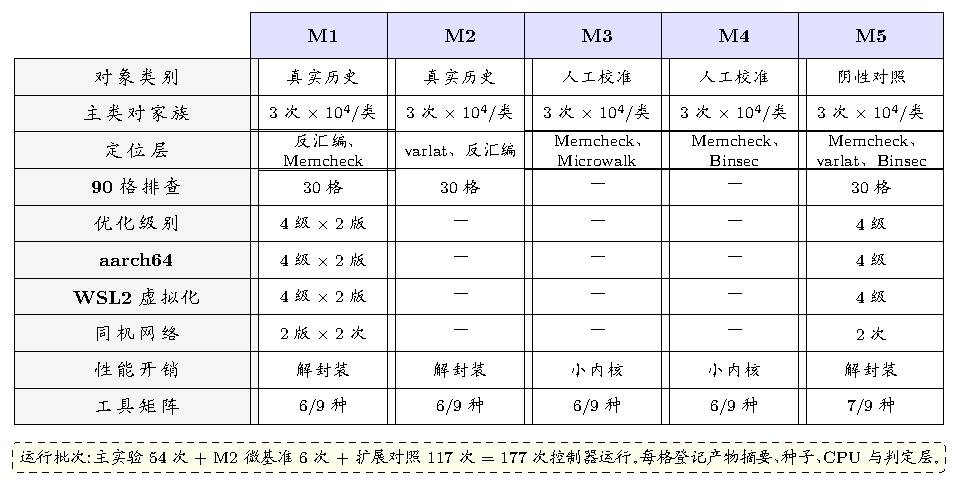
\includegraphics[width=0.98\textwidth]{assets/fig4.pdf}
\caption{实验矩阵与运行批次}
\label{fig:matrix}
\par\smallskip
{\footnotesize 图注：五个模块、三类对象、锁频/不锁频、优化级别、架构与网络各自独立登记。矩阵的空格表示该模块在该类实验中没有对象，不表示未执行；未执行项在正文单列。}
\end{figure}

矩阵的每一格都绑定产物摘要、种子、CPU 与判定层。图~\ref{fig:matrix} 证明每一项结论都有对应的对象、环境与判定层；它不证明这些组合覆盖了所有环境，矩阵之外的组合没有数据。

正式采集分三批：平台家族 54 次控制器运行、M2 微基准 6 次、收尾 117 次（格式破损 18、性能 54、优化级别 36、锁频对照 9），合计 177 次。一次控制器运行是一次经过计划校验、频率放行与退出恢复的采集单元；M1 的封存数据不计入这 177 次，统计口径仍按当时冻结的家族。% A-31 % B-08

被拒绝的运行与未执行项分开登记。优化级别实验中有 1 次运行因 20 次探针的频率跨度 54,629 kHz 超过 50,000 kHz 阈值被控制器拒绝，换名重跑后计入；性能批次有 1 次运行跨度 50,310 kHz 略超阈值，20 个采样值仍在 ±2\% 带内，已如实登记。未执行项包括 GCC 对照、-O1/-Oz/-Og 三个优化级别、第三架构、isolcpus 与关闭 SMT、真实远程网络、第二台测量机、Microwalk 扩展到 M1/M2、Binsec 覆盖完整解封装、面向 CI 的回归门禁。这些项目只写“未执行”，不并进阴性。% A-26 % A-31

M1 的数据是同一台机器、同一套锁频规程下的前期封存结果，不是与 M2--M5 同一批采集；引用时单独标注。第二台真实测量机没有部署，所有时间结论只来自这一台 x86\_64 裸金属；aarch64 只构成第二架构，不是第二台测量机（3.11）。这两条决定适用范围。% A-01

\subsection{功能与语义等价测试}
% A-33 M1 功能向量
% A-34 M2/M3/M5 功能向量
% A-35 修复等价与额外输入

功能测试先证明“被测对象仍是 ML-KEM”，再谈侧信道；修复版本必须与未修版本逐字节等价。被测对象的口径并不相同：M1 是 FIPS 203 初始公开草案的可移植 C 路径，M2 是历史 Kyber768 参考实现，M5 对应最终标准。三者的功能向量不能混用同一套期望值；M1 的密钥生成差异就是口径差异的直接结果。\cite{fips203}

表~\ref{tab:function} 把五组功能结果列在一起。% A-33--A-35

\begin{table}[H]
\centering
\caption{功能正确性与语义等价}
\label{tab:function}
{\small
\begin{tabularx}{\textwidth}{|>{\raggedright\arraybackslash}p{2.5cm}|>{\raggedright\arraybackslash}p{3.5cm}|>{\raggedright\arraybackslash}X|}
\hline
对象 & 测试向量 & 结果与说明 \\
\hline
M1 两版 & NIST ACVP 转换的 ML-KEM-768 向量 & 执行 60 例通过 35：encaps 25/25、decaps 10/10（含 5 例隐式拒绝）通过；keygen 0/25 未通过，原因是 liboqs 0.10.0 实现 FIPS 203 初始公开草案，其 K-PKE.KeyGen 的哈希输入不含最终稿新增的参数集域分隔字节；另有 20 例密钥校验因封装层无对应入口记为不适用 \\
\hline
M2 两版 & Kyber round3 官方 KAT & 100/100；普通构建与 ASan/UBSan 构建测试各 7/7 \\
\hline
M3、M5 & NIST 独立向量 & 各 80/80（含隐式拒绝用例） \\
\hline
修复等价性 & 同一驱动、同一公开输入 & 三对“未修 / 已修”实现的逐例输出摘要 diff 全空 \\
\hline
额外输入 & 一半随机密文、一半逐字节篡改 & 隐式拒绝 1000/1000 按 FIPS 203 或 round3 规范生效 \\
\hline
\end{tabularx}
\par\smallskip
{\footnotesize \textbf{表注：}修复前后功能等价；M1 keygen 0/25 来自 ipd 与最终稿的域分隔差异，不是实现错误。}
}
\end{table}

keygen 0/25 需要单独解释。liboqs 0.10.0 实现的是 FIPS 203 初始公开草案，草案的 K-PKE.KeyGen 在哈希输入中没有最终稿新增的参数集域分隔字节；用最终稿生成的向量去核对，密钥生成必然对不上。这是标准版本差异，不是实现错误。0/25 是标准版本差异，35/60 是可核对的通过数；两种简化都会改变对象口径。

这 60 例的构成需要写清楚。encaps 25/25 覆盖封装路径的接受分支；decaps 10/10 里含 5 例隐式拒绝，覆盖比较失败后返回假密钥的路径；keygen 0/25 全部落在密钥生成；另有 20 例密钥校验因为该封装层没有对应入口，只能记为不适用。35 通过、25 未通过，合计 60；另有 20 例不适用，单列，不与这 60 例混算。这个口径与台账的四种状态一致：不适用不是失败，也不是通过。

20 例密钥校验记为不适用，是因为该封装层没有对应入口，不是测试没做。不适用与未通过的区别在报告里必须写清楚：前者是“这个接口不提供这项检查”，后者是“提供了但结果不对”。把 20 例不适用并进 35/60 的通过率，会把分母弄错；把 0/25 的 keygen 并进“实现错误”，会把标准版本差异写成缺陷。

M2 用 Kyber round3 官方 KAT，100/100；普通构建与 ASan/UBSan 构建各 7/7。M3 与 M5 用 NIST 独立向量，各 80/80，含隐式拒绝用例。三套对象的向量来源不同，是因为它们的标准版本不同：M2 是历史 Kyber768，只能用 round3 的 KAT；M5 对应最终标准，用 NIST 向量；M3 基于 M5 基线，向量与 M5 同源。把三套向量混在一起统计“总通过率”没有意义，表~\ref{tab:function} 因此按对象分行。

三对未修/已修实现的逐例输出摘要 diff 全空，说明修复没有改动算法语义。修复涉及三类改动：把分支改成掩码选择、把除法改成乘法与移位、把人工夹具的查表或提前返回改成固定路径；改动只落在执行路径上，不落在输出上。逐例摘要 diff 比“再跑一遍 KAT”更强：KAT 只比较最终共享密钥，摘要 diff 还把中间输出与返回码一起比较；任何一处字节变化都会留下痕迹。

1000 例额外输入（一半随机密文、一半逐字节篡改）中，隐式拒绝 1000/1000 按 FIPS 203 或 round3 规范生效；这条测试覆盖的是失败路径，不是接受路径。随机密文检验一般路径上的解析与拒绝，逐字节篡改检验比较逻辑在单个字节不同时的行为；两类输入都不接触私钥内容，只检验失败路径是否按规范返回假密钥。1000/1000 说明失败路径没有被修复破坏，不说明失败路径的耗时与成功路径不可区分；后者属于 3.3 的计时层。

ASan/UBSan 构建的 7/7 是另一条证据。普通构建只证明功能正确，消毒器构建还要证明没有越界、未定义行为与内存错误；7/7 说明修复没有引入这类问题。消毒器构建的性能不适合计时，功能测试只在普通构建上做计时，两者分开登记。

表~\ref{tab:function} 证明三对修复没有改动算法语义，M1 的 0/25 是标准草案版本差异；它不证明任何实现是常数时间，也不证明这些向量覆盖了全部输入。功能等价是侧信道结论的前提：如果修复改变了输出，“修复后不可区分”就可能只是算法变了，而不是泄漏消失了。功能测试的另一条边界是向量集：NIST ACVP 与 round3 KAT 覆盖规范路径，不覆盖所有畸形输入；畸形输入由 3.8 的两组对照单独处理。向量集的来源与版本见附录 B，功能结论只覆盖这些向量集。

\subsection{端到端可区分性}
% A-01--A-08 五模块主结果
% A-09--A-14 统计判定与 dudect
% A-16 RTLF
% B-01 效应占比
% B-04 RTLF 数据集
% B-07 主类对样本

预注册 Holm 家族中，只有 M1 未修主类对与 M4 vulnerable 臂被拒绝；M2、M3、M5 的家族均未拒绝任何检验。图~\ref{fig:forest} 把七个类对的均值差与 95\% 区间放在同一把尺子上：M1 未修与 M4 vulnerable 的区间不含 0，其余五个区间含 0。% A-01--A-08

\begin{figure}[htbp]
\centering
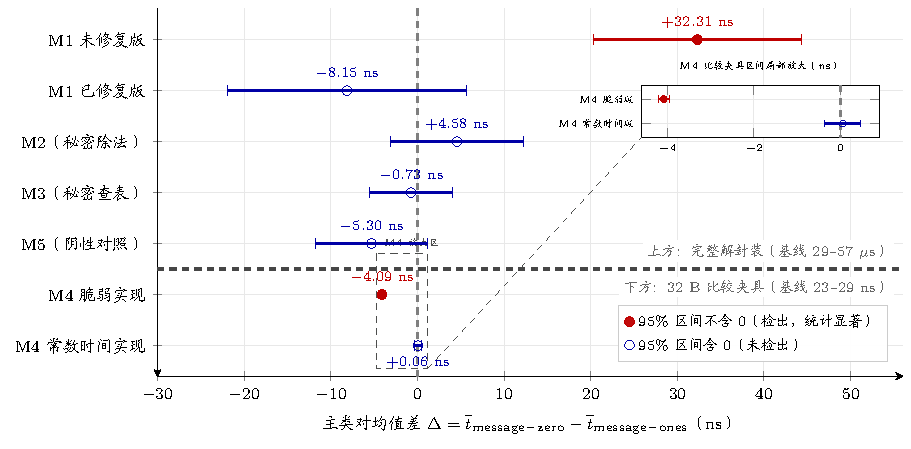
\includegraphics[width=0.98\textwidth]{assets/fig5.pdf}
\caption{五模块主类对均值差与 95\% 区间}
\label{fig:forest}
\par\smallskip
{\footnotesize 图注：M1 与 M4 vulnerable 臂区间不含 0，其余模块未检出。区间为三次独立运行的逆方差合并结果；M4 是 32 B 比较调用，数值不可与完整解封装直接比较。}
\end{figure}

家族的构成决定了门槛。M1、M2、M3、M4 各 6 项，M5 3 项；每个模块的 6 项来自 3 次独立运行 $\times$ 2 个版本或臂。Holm 是逐步下降校正：家族内 $p$ 值升序排列，第 $i$ 个与 $\alpha/(m-i+1)$ 比较，一旦某一步不拒绝就停止。M1 的 $m=6$，最小 $p$ 的门槛是 $0.05/6\approx0.00833$；M4 的 $m=6$，门槛相同；M5 的 $m=3$，门槛是 $0.0167$。门槛在采集前写进计划，不随观测到的 $p$ 值变化。

先看 M1。三次独立运行的均值差为 +39.337、+31.117、+22.337 ns，三个 95\% 区间都不含 0；逆方差合并为 +32.311 ns，区间 [20.282, 44.339]。Holm 家族 $m=6$，最小 $p=1.30\times10^{-5}$，低于阈值 0.00833，是家族中唯一被拒绝的检验。效应占完整解封装均值 57,010.7 ns 的 0.0567\%，约 0.06\%；32 ns 在 10 ns 的最小步进下只有 2--3 个分辨率单位，单次调用不可分辨，结论靠每类 10,000 次、三次运行。dudect 的最大 $t$ 为 26.41、40.64、14.92，RTLF 在未修臂报告差异、在已修臂未报告差异，方向与 Welch 检验一致。% A-01 % A-09 % A-11 % B-01 % B-07

三次运行的方向一致，比单次拒绝更重要。三次分别换种子、换物理核：同核不同种子两次，同种子不同核一次；三次都给出正号、区间都不含 0，说明结论不依赖某一组输入或某一个核的局部状态。反过来说，如果三次方向不一致，即使合并后拒绝零假设，也要按预注册规则登记为不稳定，不能挑一次最有利的运行写进结论。M1 的三次结果没有触发这条规则。

效应大小与统计判定要分开读。32.311 ns 只占 57,010.7 ns 的 0.06\%，在绝对值上很小；它的统计判定来自每类 10,000 次、三次运行与预注册家族，不来自效应大。把“拒绝零假设”当成“效应大”会误导读者：这个效应在单次调用上不可分辨，在本地锁频、大样本下才可分辨；远程或小样本下可能完全看不到。

M4 的阳性更强。vulnerable 臂三次运行的原始 $p$ 为 0、$9.23\times10^{-25}$、$3.14\times10^{-22}$；0 是双精度下溢，正文写“小于最小可表示值”。Holm 家族 $m=6$，拒绝 3 项，全部来自 vulnerable 臂；合并差 $-4.089$ ns，区间 [$-4.215$, $-3.963$]。ct 臂合并差 +0.055 ns，区间 [$-0.363$, 0.473]，原始 $p$ 为 0.386、0.438、0.399，三项都不拒绝。dudect 的最大 $t$ 从 vulnerable 臂的 356.6、396.9、395.6 降到 ct 臂的 2.06、1.90、2.27。M4 是 32 B 比较调用，用原始单调时钟计时，数值不可与完整解封装的 32 ns 直接比较。% A-06 % A-07 % A-10 % A-12

M4 的区间窄得几乎看不见，是因为比较调用的方差远小于完整解封装。32 B 比较的基线远小于完整解封装，单次调用没有 NTT、采样与序列化的开销，噪声源少，标准误小；同样的每类 10,000 次，M4 的 MDE 只有 0.19--1.19 ns，而完整解封装的 MDE 在几十纳秒。区间窄不等于效应大：$-4.089$ ns 在绝对值上只有 M1 的八分之一，但它的信噪比高，所以在图上反而更醒目。

效应绝对值与可检出性强弱并不同向：M4 只有 4 ns，MDE 低到 1.47 ns，信噪比高；M1 的 32 ns 更大，完整解封装的方差也大，MDE 高到 31.39 ns，信噪比反而低。判断可区分性要看区间与 MDE，不看点的位置。

M2 的家族没有拒绝项。完整解封装合并差 +4.58 ns，区间 [$-3.08$, 12.25]，含 0；按臂描述，未修臂 +12.35 ns、已修臂 $-11.20$ ns，$I^2=58.3\%$。两个方向相反、异质性偏高，读作臂间漂移，不读作除法泄漏。按臂合并值不属于预注册的 6 个家族成员；家族成员是三次运行的逐次检验，按臂值只作描述。

主类对不是为除法操作数设计的：message-zero 与 message-ones 只让解密消息的位不同，除法的被除数是否随消息位系统变化没有控制；这一条在 3.7 的检测预算里再展开。M2 的 dudect 阳性落在已修臂（4.68、3.05、3.66 对 36.27、30.94、61.91），不能归因于除法；3.12 把它作为单工具误读的例子。% A-03 % A-04 % A-13

M2 的按臂描述还暴露了主类对的设计问题。未修臂 +12.35 ns、已修臂 $-11.20$ ns，两个方向相反；如果主类对真的触发了除法，两个臂应该同向，只是幅度不同。方向相反说明两臂的差异更多来自运行间的漂移，而不是同一个机制。$I^2=58.3\%$ 是这种漂移的量化：合并估计只作描述，判定仍以预注册的 Holm 结果为准。

M3 的合并差为 $-0.73$ ns，区间 [$-5.56$, 4.10]，Holm 拒绝 0；M5 的合并差为 $-5.30$ ns，区间 [$-11.77$, 1.16]，家族 $m=3$，拒绝 0。M5 是阴性对照，未检出只说明在本机、本编译产物、本类对与每类 10,000 次的预算下没有看到可区分差异；它不是安全性结论。M3 是人工夹具，on/off 两臂只差人工查表，计时层未检出说明该机制在本机没有被端到端计时分辨出来，不说明查表没有风险。M5 的 dudect 最大 $t$ 为 2.10、1.98、2.82，也在阈值 10 以下，与 Welch 检验同向。% A-05 % A-08 % A-14

M5 的 3 项家族成员没有一项接近门槛：合并差 $-5.30$ ns，区间跨 0，dudect 最大 $t$ 只有 2.10、1.98、2.82，远低于阈值 10。三个来源都指向“本预算下未检出”，但没有一个能证明“没有机制”。阴性对照的价值在于检查工具会不会冤枉好人，不在于证明好人一定没问题。

端到端 $\Delta$ 的符号不能按分支代价模型解释。符号受二进制布局、对齐与指令调度影响；主实验的 +32.3 ns 与优化级别实验的 $-26.16$ ns 采用不同的 $\Delta$ 定义方向，同一机制在不同构建中给出相反符号。本作品只按“区间是否含 0”判定可区分性，不解释符号，也不把符号当作机制证据。% A-01 % A-26

图~\ref{fig:forest} 的纵轴按模块排列，不按 p 值排列。按 p 值排列会让读者以为“上面的模块更重要”；按模块排列，读者可以先看同一模块的未修/已修或不同臂，再看跨模块的比较。M4 的两行挨在一起，就是为了让 vulnerable 与 ct 的区间直接对照。

族外检验给出另一层信息。RTLF 在 $\alpha=0.01$、固定种子与 10,000 次 bootstrap 的设置下，对 M2--M5 的 42 个数据集给出 30 个未检出、12 个检出；检出的 12 个集中在 M2 主类对与 M4 vulnerable 臂及其对照，M3 的 12 个与 M5 的 6 个数据集全部未检出。RTLF 与 Welch 检验比较的对象不同：前者比较分布与分位，后者比较均值；两者不互相替代，也不并入同一个 Holm 家族。\cite{rtlf} % A-16 % B-04

族外检验不并入 Holm，是因为零假设与错误控制方式不同。RTLF 用 bootstrap 控制第一类错误，dudect 用最大 $t$ 的经验阈值，Mona 用箱体分离；把三者塞进同一个 Holm 家族，会得到一个既不是 0.05 也不是 0.01 的混合错误率。它们的位置是交叉印证：同向时增加信心，反向时提示输入类或环境有问题，而不是投票。

dudect 也属于族外。它用在线 $t$ 检验，阈值是上游默认的 10，不转换成 $p$ 值参与 Holm；M1 未修在三批内停止并报告泄漏，已修跑满批次仍为“可能常数时间”；M4 vulnerable 三次都报告泄漏，ct 臂三次都未报告；M5 三次都未报告。\cite{dudect}

主类对是同一份确定性密文的 10,000 次重复，单次运行的区间反映测量噪声，不是密文间的变异；跨种子复测部分弥补这一点，但不等价于在每类内部使用大量不同密文。10 ns 的量化尺度下，32 ns 的效应只有 2--3 个分辨率单位；这不是把 32 ns 说小，而是说明为什么必须用大样本与预注册家族。图~\ref{fig:forest} 不能回答“效应从哪来”。区间只说明两类密文的均值差在本预算下是否可区分，不说明差异来自哪条指令；M1 的差异要结合 3.4 的分支定位才能归因，M4 的差异要结合 3.6 的 ct 臂对照才能确认。把图上的点直接读成“某条指令的代价”，会把统计证据与机制证据混在一起。

图~\ref{fig:forest} 证明在本机、本预算下哪些类对可区分；它不证明机制存在或不存在，不证明可远程利用，也不把 M5 的未检出写成安全。

\subsection{函数级泄漏定位}
% A-17 M1 定位
% A-18 M2 定位
% A-19 M3 定位
% A-20 M4 定位
% A-21 M5 定位
% A-23 残留分支

定位层把每个阳性落到函数、指令或源码行；定位阳性与计时阳性是两件事，必须分开登记。同一个模块可以在定位层阳性、在计时层未检出，M2 就是这种组合；反过来，计时层阳性也必须能回到一条具体指令，否则无法判断修复是否生效。

动态检查的工作方式决定了它能回答什么。秘密标记把私钥中参与解密的 1152 B 与隐式拒绝秘密的 32 B 标成“未初始化”，公开输入保持已初始化；程序在标记下跑完整解封装，工具报告“以秘密值为分支条件”与“以秘密值为访存下标”两类事件。错误数是动态命中次数，上下文数是去重后的源码位置数；同一个循环执行 1280 次会报 1280 个错误，但只算 1 个上下文。报告里同时给两个数，是为了让读者看到“问题分布”而不是“执行次数”。

M1 未修版本的消息编码函数里，编译器把源码中的掩码选择还原成按位测试后条件跳转：先测试消息位，再由条件跳转决定是否写入系数。私钥标记下，Memcheck 报告 1 个秘密条件跳转。修复版本改成置位加条件传送：同一个按位测试之后用置位指令物化消息位，再调用 16 位条件传送辅助函数完成选择；反汇编里条件跳转消失，Memcheck 报告 0。两版的功能输出逐字节相同，说明消失的是执行路径，不是语义。\cite{clangover} % A-17

反汇编上的差别可以逐条读。未修版本是“按位测试 + 条件跳转”：测试结果决定是否跳过写系数；修复版本是“按位测试 + 置位 + 调用条件传送辅助函数”：测试结果被物化成 0 或 1，辅助函数用取负、异或、与、再异或完成选择，不产生依赖秘密的跳转。两条路径的指令数不同，但都不依赖秘密；修复的代价是多了几条算术指令与一次调用，收益是分支消失。

M2 的三处整数除法分别落在消息解码、多项式压缩与向量压缩。未修版本在可变时延检查下报告 1280 errors / 3 contexts；修复版本用乘法与移位替代除法，除法计数从 3 降到 0，可变时延报告 0/0。关闭可变时延检查时，两版都报告 0，说明普通 Memcheck 看不到除法：它只检查秘密是否进入分支或访存下标，不检查指令时延是否随操作数变化。1280 次错误来自同一源码位置的多次执行，3 个上下文才是问题分布。\cite{kyberslash} % A-18

三处除法各自对应一个上下文：消息解码一处、多项式压缩一处、向量压缩一处。三处的被除数都来自解密消息或重加密中间值，除数都是公开模数；修复用乘法与移位替代除法，三处的除法计数同时降到 0。varlat 的 1280 次错误分布在三个上下文上，说明三处都被执行到；如果只修一处，另外两处仍会报错。

可变时延检查的边界也要写清楚。它标记的是“秘密操作数进入可变时延指令”，不是“这条指令一定产生可测差异”。除法在 x86\_64 上的时延是否随操作数变化，取决于处理器微架构、操作数大小与流水线状态；工具能指出“这里有秘密操作数”，不能指出“这里一定泄漏多少纳秒”。M2 的定位阳性与计时未检出并不矛盾：前者是机制层，后者是端到端层，两层的判据不同。

M3 的 Memcheck 报告 1280 errors / 2 contexts，全部落在人工插入的秘密下标读取；off 臂去掉查表后为 0/0。Microwalk 在同一对象上给出互信息 1.922 bits，是全场最高；off 臂为 0.722 bits。Microwalk 只有 5 个公开 testcase、没有重复、没有统计检验，互信息只作定位层的独立佐证，不升级为泄漏量。\cite{microwalk} % A-19

互信息 1.922 bits 的含义是“看过这条指令的访存地址后，对秘密的不确定性平均减少 1.922 bit”。它是关联强度，不是泄漏量；1.922 bits 不能换算成“恢复多少位密钥”。Microwalk 的 5 个 testcase 只覆盖 5 组公开输入，没有重复、没有统计检验；互信息高只说明这条指令与秘密关联强，不说明攻击者能利用它。

M4 的 Memcheck 报告 32 errors / 1 context，落在提前返回的比较行。Binsec 在同一对内核上判 vulnerable 为 insecure，反例地址对应提前返回行；ct 臂判 bounded secure，路径探索完整。把搜索深度限为 5 时，工具返回 unknown，而进程退出码仍是 0；只看退出码会把 unknown 读成安全。M4 只开了控制流与访存检查，未开乘除法检查；它的结论只覆盖这对 32 B 比较内核。\cite{binsec} % A-20

Binsec 的反例地址对应提前返回行，说明工具找到了一条“从第几个字节开始不同”的秘密相关路径。ct 臂的 bounded secure 不是“所有输入都安全”，而是“在入口、终点与公开长度 1--16 B 的范围内，没有找到秘密相关路径”；范围外的输入不在证明里。深度限 5 的 unknown 是另一个边界：工具没有证明不安全，也没有证明安全，退出码却是 0。

M5 在三种动态模式下各做 10 次完整解封装：普通 Memcheck、关闭可变时延、开启可变时延，三者都是 0 errors / 0 contexts。重加密路径的 Binsec 检查中，比较步骤 1088/1088 条路径完成，消息编码 1/1 条路径完成，没有秘密相关控制流；同一配置下 M4 的脆弱内核报告 insecure，说明工具在这套配置里不会把已知脆弱代码判成安全。Binsec 只覆盖重加密比较与消息编码，不覆盖完整解封装的所有性质。% A-21

三种动态模式的分工不同：普通 Memcheck 看分支与访存下标，关闭 varlat 看同一组输入下是否有普通标记错误，开启 varlat 看除法等可变时延指令。三者都是 0/0，说明在这组输入上没有这三类问题；换一组输入，未执行的路径不会被报告。Binsec 的 1088/1088 与 1/1 是路径计数，不是“所有路径都安全”的证明；它只覆盖重加密比较与消息编码两个内核。

定位层的输出要归一化成同一种证据记录：工具与版本、输入集合、命中位置、上下文数、处置结论。同一位置被两类工具命中记两条证据，只有一类命中时保留但不升级为“确认”；归因要求同一位置至少在三次运行中的两次出现，且换种子后仍出现，只出现一次的命中记为“待复核”。

五类工具的回答范围可以排成一条链：反汇编回答“机器码里有没有目标指令形态”，不回答运行时是否真的触发；秘密标记回答“秘密是否进入分支或访存下标”，不回答可变时延指令；可变时延检查回答“秘密是否进入除法等指令”，不回答缓存与分支；轨迹互信息回答“哪些指令与秘密的关联最强”，不回答时序可利用性；有界符号执行回答“给定范围内是否存在秘密相关路径”，不回答范围外的行为。链条上的每一环都只回答一个问题，合起来才覆盖机制层的几个侧面。

这组结果证明机制在该产物、该输入、该工具下存在或不存在；它不证明完整解封装一定可测，也不证明未命中的输入没有机制。M4 是 32 B 比较夹具，不外推到完整解封装；Binsec 是有界验证，只覆盖给定内核与公开长度范围；动态工具只覆盖执行过的输入，0 条报告不是安全性结论。定位阳性与计时阳性分开登记：M1 两层都阳性，M2 定位阳性、计时未检出，M3 定位阳性、计时未检出，M4 两层都阳性，M5 两层都未检出。

\subsection{泄漏源全流程排查}
% A-22 90 格汇总
% A-23 残留分支
% B-06 90 格分解

90 格排查把“六类来源 $\times$ 五个步骤 $\times$ 三个实现”逐格判定。5 个“存在”之外，还有一处更需要解释：官方修复后仍残留的同源分支。判定只有四种：存在、不存在、不适用、未检查。判“存在”必须给出可指认的函数、指令或源码位置以及触发它的输入；判“不存在”必须写明用了哪种检查、覆盖了哪些输入；判“不适用”要求该机制在这一步骤上不可能出现；判“未检查”单列，不并入阴性。

五个步骤是解密、哈希派生、重加密、比较与隐式拒绝。把哈希派生从重加密里拆出来，是因为哈希路径上的问题如果被记到重加密名下，定位只能停在“重加密有问题”这一层；拆开后，每一步都有自己的函数与指令，修复后可以逐格复查。六类来源是敏感分支、提前返回、可变时延指令、秘密下标、数据相关循环与异常路径；三个实现是 M1、M2 与 M5，人工夹具 M3、M4 不进入这张表，因为它们只覆盖单一机制，放进 90 格会把夹具结论与真实实现混在一起。

\setcounter{algorithm}{7}
\begin{algorithm}[H]
\caption{90 格泄漏源排查}
\label{alg:sweep}
\begin{algorithmic}[1]
\Require 实现集合 $\{$M1, M2, M5$\}$；步骤集合 $\{$解密, 哈希派生, 重加密, 比较, 隐式拒绝$\}$；六类来源
\Ensure 90 格判定与证据
\For{每个实现、每个步骤、每类来源}
  \State 检查源码与反汇编
  \State 运行 Memcheck、varlat、Microwalk、Binsec（适用时）
  \State 判定：存在 / 不存在 / 不适用 / 未检查
  \State 记录函数、源码行或指令地址、证据编号
\EndFor
\State 汇总：存在 5 / 不存在 75 / 不适用 10 / 未检查 0
\end{algorithmic}
\end{algorithm}

算法~\ref{alg:sweep} 回答的是每一格在给定产物与检查手段下是否存在机制；它不回答该机制是否能被端到端计时分辨。表~\ref{tab:sweep} 给出汇总。% A-22 % B-06

\begin{table}[H]
\centering
\caption{全流程排查汇总}
\label{tab:sweep}
{\small
\begin{tabularx}{\textwidth}{|>{\raggedright\arraybackslash}p{4.4cm}|*{5}{>{\centering\arraybackslash}X|}}
\hline
实现 & 存在 & 不存在 & 不适用 & 未检查 & 小计 \\
\hline
M1 liboqs 0.10.0（未修 / 982c762） & 1 & 26 & 3 & 0 & 30 \\
\hline
M2 Kyber768（a621b8d / 272125f） & 3 & 24 & 3 & 0 & 30 \\
\hline
M5 mlkem-native b3ba7b3 & 1 & 25 & 4 & 0 & 30 \\
\hline
合计 & 5 & 75 & 10 & 0 & 90 \\
\hline
\end{tabularx}
\par\smallskip
{\footnotesize \textbf{表注：}90 格 = 5 存在 + 75 不存在 + 10 不适用 + 0 未检查；M1 1、M2 3、M5 1。分模块行按 30 减去存在与不适用导出（B-06），全表见附录 F。}
}
\end{table}

5 个“存在”逐格如下。M1 未修/重加密/敏感分支：消息编码函数中的按位测试后条件跳转，Memcheck 1 个上下文。M2 未修/解密/可变时延指令：消息解码中的整数除法。M2 未修/重加密/可变时延指令：多项式压缩与向量压缩中的整数除法。M2 未修与已修/重加密/敏感分支：消息编码函数中的同一分支在两版中都存在。M5/隐式拒绝/提前返回：上游设计行为，按有界例外登记。% A-22

这 5 格不是按“看起来可疑”选的，而是按“有可指认的函数、指令或源码位置，且有触发输入”选的。判“存在”的门槛比判“不存在”高：后者只要检查手段覆盖了输入且没有命中，前者必须给出触发路径。5 格里有 4 格在 M1/M2，1 格在 M5；M5 的那一格是上游设计行为，按有界例外登记，不算缺陷。

“不适用”的 10 格不是“没查到”，而是机制与步骤的组合不可能出现。例如某一步没有异常处理，异常路径一列就判不适用；某个函数不可能失败，提前返回一列就判不适用。判“不适用”要求给出“为什么不可能”的理由，而不是因为没时间查。10 格不适用集中在 M1 与 M2 的异常处理组合，M5 有 4 格，是因为它的错误路径设计与上游不同。% A-22

第 4 格是排查中最需要解释的一格。KyberSlash 官方修复提交只消除了除法，消息编码函数中的按位测试后条件跳转仍在；未修与已修两侧的指令字节逐字节相同，秘密标记 Memcheck 在两侧各报 256 errors / 1 context。该函数体与 M1 未修版本相同，即与 clangover 同源。主类对 message-zero 与 message-ones 恰好使该分支在每个消息位上走系统性不同的路径，这为 RTLF 在 M2 两臂主类对上均报告分布差异、而在格式破损对照类对上未报告提供了一个机制层面的候选解释。\footnote{官方修复提交 272125f；另一提交 dda29cc 只修第一处。提交号仅用于定位历史版本。} % A-23

这条观察有三条边界。第一，本作品没有做逐指令时序归因，不能把 RTLF 观测到的差异直接归于该分支。第二，已修臂三个种子的类间偏移符号翻转（+21.7、$-17.1$、$-15.5$ ns），离散度约为未修臂的 1.9 倍，未受控漂移仍是并列因素。第三，在同一分支存在的情况下，M2 预注册家族仍为 Holm 拒绝 0，其原因（-Oz 与 -Os 的代码布局差异、M2 噪声水平更高）尚未分离，列为待补实验。% A-23

90 格的证据字段包括实现与产物摘要、步骤、来源类别、判定、函数名或指令地址、触发输入、检查手段与证据编号。换一个人按同样字段复核，结论应当一致；判“存在”的格子必须有触发输入，没有触发输入的“存在”只能算“疑似”，汇总时降级为“未检查”。这套字段让 90 格既是排查表，也是审计清单。

三条边界指向同一个结论：这是候选解释，不是因果证明。要把候选解释升级为因果，需要逐指令计时、把分支单独抽出来做微基准，或者在关闭分支的构建上复测；本作品没有做这三件事。把“观察到的同源分支”写成“该分支导致了计时差异”，会把机制层观察与因果归因混在一起；把“Holm 拒绝 0”写成“分支不存在”，则是把统计结论与产物结论混在一起。

这是历史提交上的机制层观察，不是新漏洞；未修复、未复测，列为后续工作第一位。当前上游代码是否仍有此问题不在本作品验证范围内；这条观察停在机制层，不构成新漏洞的结论。

把这条观察放进报告，是因为它能回答“官方修复是否等于产物常数时间”。答案是否定的：修复消除了除法，但没有消除同源分支；分支是否可被计时利用，本作品没有做因果归因，只把它登记为候选解释。这个区分很重要：机制层观察可以写，因果结论不能写。

排查表的“不存在”也不是“永远不存在”。它只在给定产物、给定输入、给定工具下成立；换编译器、换优化级别、换输入类，结论可能变化。3.10 的 12 格就是例子：同一份源码在 -Os 有分支，在 -O0 没有；如果只查一个级别，就会把“这个级别没有”写成“这个实现没有”。

表~\ref{tab:sweep} 证明在给定产物、输入与工具下 90 格中没有发现其他机制，且没有把未做写成阴性；它不证明这些实现是常数时间。90 格的“不存在”只在所用检查手段的覆盖范围内成立：反汇编看不到运行时时序，动态工具只覆盖执行过的输入，有界验证只覆盖给定范围。源码层面的常数时间写法，经过编译器、链接器与指令选择之后不一定仍是常数时间产物；判定必须落在实际二进制上，并随编译条件、架构与测量预算一起表述。

\subsection{防护前后复测}
% A-01/A-02 M1 前后
% A-06/A-07 M4 前后
% A-11/A-12 dudect
% A-18 M2 定位
% A-19 M3 定位
% A-25 开销
% A-36 泄露渠道审计

M1 与 M4 在定位层和计时层都实现了“修复前可区分、修复后不可区分”；M2 只能在定位层说“机制消失”。表~\ref{tab:beforeafter} 把四个模块的防护前后放在同一张表上，证据层一列写明结论属于哪一层。% A-01 % A-02 % A-06 % A-07 % A-11 % A-12 % A-18 % A-19

\begin{table}[H]
\centering
\caption{防护前后对比}
\label{tab:beforeafter}
{\small
\begin{tabularx}{\textwidth}{|>{\raggedright\arraybackslash}p{1.2cm}|>{\raggedright\arraybackslash}p{3.5cm}|>{\raggedright\arraybackslash}p{5.2cm}|>{\raggedright\arraybackslash}X|}
\hline
模块 & 证据层 & 防护前 & 防护后 \\
\hline
M1 & 完整解封装（合并） & +32.311 ns [20.282, 44.339]，3/3 区间不含 0 & $-8.150$ ns [$-21.916$, 5.616]，3/3 区间含 0 \\
\hline
M1 & dudect 最大 $t$ / RTLF & 26.41、40.64、14.92 / 有差异 & 1.15、1.12、1.31 / 无差异 \\
\hline
M1 & 定位 & 按位测试后条件跳转；Memcheck 1 & 置位 + 条件传送；Memcheck 0 \\
\hline
M2 & 定位 & 三处整数除法；varlat 1280 / 3 & 除法计数 0；varlat 0/0 \\
\hline
M2 & 完整解封装（按臂描述） & +12.35 ns [2.98, 21.71] & $-11.20$ ns [$-24.56$, 2.15] \\
\hline
M3 & 定位 & Memcheck 1280 / 2；1.922 bits & Memcheck 0/0；0.722 bits \\
\hline
M4 & 比较调用 & $-4.089$ ns [$-4.215$, $-3.963$]；dudect 356.6--396.9 & +0.055 ns [$-0.363$, 0.473]；dudect 1.90--2.27 \\
\hline
\end{tabularx}
\par\smallskip
{\footnotesize \textbf{表注：}M1、M4 两层前后对照完成；M2 仅定位层机制消失。M2 的计时层在防护前就未检出，没有“降低”的基线可比较；M2 的按臂值只作描述，不参与 Holm。}
}
\end{table}

复测的前提是同一规程。防护前后的计时使用同一个计时循环、同一个预注册家族、同一个功能门；修复后的二进制重新记录摘要，但输入类、样本量、种子与核不变。换一样东西，“修复后不可区分”就可能来自环境变化，而不是防护生效。M1 的修复版与未修版在同一台机器、同一锁频工作点上各跑三次；M4 的 ct 臂与 vulnerable 臂在同一驱动下各跑三次；M2 与 M3 同样成对。

四层前后对照的判据要分开写。定位层的完成判据是“目标机制在产物中消失且动态检查为 0”；计时层的完成判据是“修复后区间含 0 且族外检验不再报告”；功能层的完成判据是“输出逐字节相同”；性能层的完成判据是“开销有区间、可复算”。四层都过，才能说“这个机制在修复后不可区分”；只过一层，只能写那一层。M1 与 M4 四层都过，M2 只过定位层，M3 过定位层与功能层、计时层未检出。

M1 的修复把消息编码分支换成掩码选择。计时层三次运行有三次区间含 0，合并 $-8.150$ ns、区间 [$-21.916$, 5.616]；dudect 最大 $t$ 从 26.41、40.64、14.92 降到 1.15、1.12、1.31；定位层从 1 个秘密条件跳转降到 0。功能层三对输出 diff 全空，性能开销 +1.51\% [1.36, 1.65]。四层放在一起，才能说“这个机制在修复后既不在产物里，也不在计时上可区分”。

M1 修复后的点估计是 $-8.150$ ns，不是 0；区间含 0，说明这个负值在噪声范围内。把点估计写成“修复后快了 8 ns”会误读：区间跨 0，不能拒绝“没有差异”。修复后的 dudect 最大 $t$ 也只有 1.15、1.12、1.31，远低于阈值 10；三个来源都指向“不可区分”，但没有一个能证明“绝对没有差异”。

M4 的 ct 臂把提前返回改成遍历全部字节、循环结束统一判断。计时层合并 +0.055 ns、区间 [$-0.363$, 0.473]；dudect 最大 $t$ 从 356.6、396.9、395.6 降到 2.06、1.90、2.27；定位层 Memcheck 从 32/1 降到 0/0，Binsec 从 insecure 变为 bounded secure；两臂输出逐字节相同。M4 的两层都阳性、修复后两层都阴性，是四个模块里最完整的正对照；它的边界是 32 B 比较夹具，不外推到完整解封装。

M2 只能写到定位层。除法计数从 3 降到 0，varlat 从 1280/3 降到 0/0；计时层修复前就是 +4.58 ns、区间含 0，修复后没有“降低”的基线可以比较。按臂描述 +12.35 与 $-11.20$ 的方向相反，$I^2=58.3\%$，读作漂移而不是修复效果。M2 的修复前基线本来就是未检出，写“泄漏降低”没有可比的基线。

M2 的 dudect 阳性落在已修臂，不能算作修复效果。已修臂最大 $t$ 36.27、30.94、61.91，比未修臂的 4.68、3.05、3.66 高得多；如果只看 dudect，会得出“修复引入泄漏”。把 dudect 与 Welch、varlat 交叉，才知道阳性落在已修臂、且没有定位到除法；这不是修复效果，是另一种差异。

M3 的 on/off 两版输出逐字节相同，这是先决条件：如果输出不同，计时差异可能来自语义变化，而不是查表。off 臂 Memcheck 0/0，互信息从 1.922 bits 降到 0.722 bits；0.722 仍高于 0，说明即使去掉人工查表，其他指令与秘密仍有弱关联，它是基线，不是“零”。计时层两臂都未检出。M3 的防护是去掉人工插入的查表，不是修上游代码；它证明检测链路能识别并确认一个已知机制，不证明真实库有同样缺陷。

四条防护路径的代价不同。M1 的掩码选择只多几条算术指令与一次调用，对完整解封装的开销是 +1.51%；M2 的乘法与移位替代除法反而减少指令，开销 −2.92%；M3 去掉查表，开销 +3.60% 且区间很宽；M4 的遍历全部字节把比较从“提前返回”改成“固定长度”，小内核开销 +26.21%。代价大小与防护强度不是一回事：M2 更便宜，但它的残留分支仍在（3.5）；M4 更贵，但它的两层证据最完整。

四条路径也说明“防护”不是一个动作。M1 改的是编译器还原出的分支，M2 改的是源码里的除法，M3 改的是人工插入的查表，M4 改的是比较函数的控制流；四条路径分别落在产物、源码与夹具层。把它们放在同一张表上，是为了看“同一套复测规程能不能覆盖不同层的修复”，而不是把四种修复当成同一种技术。

防护复测还包括泄露渠道审计。对 128 个源文件中的 1,048 个输出或返回调用点做静态扫描，其中 122 个接触秘密相关数据，占 11.6\%；秘密内容泄露 0 条。审计发现 1 条低危问题：功能自检分支使计时程序在不同构建下退出码不同，构成可观察信号；修复后该类问题由 1 条降为 0 条。动态差分对 7 种输入模式各运行 120 次，返回码、标准输出与标准错误逐字节一致。% A-36

防护手段与核验要一一对应。M1 用掩码选择替换分支，核验是反汇编里的条件跳转消失与 Memcheck 1→0；M2 用乘法与移位替换除法，核验是除法计数 3→0 与 varlat 1280/3→0/0；M3 去掉秘密查表，核验是 Memcheck 1280/2→0/0 与互信息 1.922→0.722；M4 用遍历全部字节替换提前返回，核验是 Memcheck 32/1→0/0 与 Binsec insecure→bounded secure。每条核验都落在产物或动态报告上，不落在“源码改了”这句话上。

泄露渠道审计与计时复测是两条独立的证据链。审计回答“日志、异常、返回码是否泄露秘密”，计时回答“耗时是否可区分”；一条过、一条不过，不能互相替代。那条低危问题由审计自己发现并修掉，说明防护过程也被审计；它不说明其他渠道没有遗漏，审计不覆盖上游第三方代码、网络路径与进程级元数据。

表~\ref{tab:beforeafter} 证明在同一规程、同一家族、同一功能门下，修复前后的可区分性发生了变化；它不证明其他环境、其他输入类也如此，也不证明修复后的实现没有其他机制。防护复测的前提是功能等价：如果输出变了，“不可区分”可能只是算法变了。真实缺陷的修复采用上游官方补丁，团队自己写的修复只落在 M3、M4 两个人工夹具上；M2 的残留分支未修复、未复测，见 3.5。

防护复测的结论只覆盖同一规程。换一台机器、换一个编译选项、换一组输入，修复后的可区分性可能不同；M1 的修复版在 -O0 到 -Os 四个级别都是 0 个秘密相关分支（3.10），这是产物层的跨级别证据，不是计时层的跨环境证据。把“四个级别都是 0”写成“所有环境都不可区分”会越过层级。

\subsection{检测预算与稳健性}
% A-15 MDE
% A-16 RTLF
% B-13 MDE 公式

“未检出”的确切含义是观测效应小于该预算下的 MDE，不是效应为 0；稳健性分析用来检查结论是否依赖均值型检验。表~\ref{tab:mde} 给出各家族的 MDE，按 $\alpha=0.05$ 与 Holm 口径两列并排。% A-15

\begin{table}[H]
\centering
\caption{各家族最小可检测效应}
\label{tab:mde}
{\small
\begin{tabularx}{\textwidth}{|>{\raggedright\arraybackslash}p{2.8cm}|>{\raggedright\arraybackslash}p{3.6cm}|>{\raggedright\arraybackslash}p{3.2cm}|>{\raggedright\arraybackslash}X|}
\hline
家族 & MDE（$\alpha=0.05$） & MDE（Holm 口径） & 判定 \\
\hline
M1 未修 & 25.27 ns & 31.39 ns & 观测 +39.34 ns（r1）超过 MDE，可检出 \\
\hline
M1 已修 & 28.63 ns & 35.56 ns & 观测 $-13.21$ ns（单次运行），小于 MDE，未检出 \\
\hline
M2 端到端 & 19.9--54.0 ns & 24.7--67.1 ns & 6 项观测值均小于 MDE，未检出 \\
\hline
M3 端到端 & 14.2--27.1 ns & 17.7--33.7 ns & 两臂观测值均小于 MDE，未检出 \\
\hline
M4 比较调用 & 0.19--1.19 ns & 最坏 1.47 ns & vulnerable 臂远超 MDE；ct 臂 0/3 超过 \\
\hline
M5 端到端 & 11.7--24.5 ns & 13.5--28.3 ns & 观测值小于 MDE，未检出 \\
\hline
\end{tabularx}
\par\smallskip
{\footnotesize \textbf{表注：}MDE 是事后功效描述，不改变已提交的判定。“未检出”的含义是观测效应小于 MDE，不是效应为 0。判定列的观测值取单次运行，合并值见 3.3 与 3.6。}
}
\end{table}

MDE 按 $(z_{1-\alpha/2}+z_{1-\beta})\sqrt{s_0^2/n_0+s_1^2/n_1}$ 计算，Holm 口径把 $\alpha$ 取为 $\alpha/m$；每类 $n=10{,}000$，功效 $1-\beta=0.80$。MDE 与样本量的平方根成反比：要把 MDE 减半，样本量要翻四倍。M2 的 MDE 24.7--67.1 ns 大于除法可能带来的效应，这是“定位阳性、计时未检出”的直接解释；主类对不是为除法操作数设计的，MDE 只能说明这个预算下看不见多大的效应，不能说明除法效应不存在。% B-13

公式里有三个假设：方差估计来自样本、均值差近似正态、功效取 0.80。每类 10,000 次下，正态近似可用；方差估计本身有不确定性，MDE 只能当量级参考，不能当精确边界。把功效从 0.80 提到 0.90，MDE 会变大；把 $\alpha$ 从 0.05 降到 0.01，MDE 也会变大。表\ref{tab:mde} 给的是 0.80 与 Holm 口径，换参数要重算。公式里的 SD 来自两臂合并的样本方差；两臂方差相差很大时，Welch 的 SE 比合并方差更稳，这也是主检验用 Welch 的原因。

逐行读表可以看到三种不同的“未检出”。M1 未修的观测 +39.34 ns 超过 MDE 31.39 ns，所以可检出；M1 已修的观测 $-13.21$ ns 小于 MDE 35.56 ns，所以未检出。M4 的 MDE 只有 0.19--1.19 ns，vulnerable 臂的观测远超它，ct 臂的观测 0/3 超过；M4 的预算足以分辨亚纳秒效应，是因为比较调用的方差小。M2、M3、M5 的观测都小于各自 MDE，未检出的含义是“这个预算下看不见”，不是“效应为 0”。

M4 的 MDE 只有 0.19--1.19 ns，是因为比较调用的方差小；这不代表 M4 的结论比 M1 强，只代表它的预算能看见更小的效应。M1 的 MDE 31.39 ns 比观测 39.34 ns 小，所以可检出；如果观测降到 25 ns，同样的预算就检不出。MDE 与观测的关系是“能不能看见”，不是“效应有多大”。

M2 的 MDE 跨度很大，是因为 6 个家族成员的方差不同。未修臂与已修臂的方差不同，三次运行的方差也不同；MDE 按每个成员自己的方差算，报告给区间而不是一个数。把 MDE 写成“25 ns”会掩盖这个跨度；写成 24.7--67.1 ns，读者才知道最坏情况下这个预算只能看见 67 ns 的效应。M2 的除法效应是否落在这个范围内，本作品没有独立估计；这正是把 M2 列为局限的原因。

稳健性分析对 64 个类对（其中 21 个为冻结家族成员）另用 p99.9 截尾均值差、中位数差与 Hodges--Lehmann 位置差三种方法复核。全样本方法与冻结家族的 $\Delta$ 最大绝对偏差为 0 ns；64 个类对中有 12 个在不同方法下发生判定翻转，家族成员 7 个、族外对照 5 个，但没有任何一个翻转改变 Holm 判定。% A-15 % A-16

12 个翻转的分布说明主结论不依赖某一种统计量。家族成员的翻转没有改变 Holm，说明主家族的门槛足够严；族外对照本来就不进 Holm，翻转只作描述。翻转集中在边缘类对，主类对的区间离 0 足够远，换方法也翻不过来。翻转来自均值型与位置型检验的功效差异：均值型对长尾敏感，位置型对长尾稳健但功效低；在 10 ns 量化下，秩方法会把大量并列值当成同秩，功效进一步下降。把 12 个翻转原样列出，比只报“稳健”更有信息量。

表~\ref{tab:mde} 与这组敏感性分析证明“未检出”有预算、结论不依赖单一均值检验；它们不证明所有方法都同意，也不证明未检出等于没有效应。MDE 不改变已经提交的 Holm 判定；把 MDE 当成精确边界，会把功效计算的不确定性藏起来。

MDE 是事后功效描述，不是事前承诺。采集前冻结的是样本量、家族与停止条件，MDE 是采集后按观测方差算出来的；它回答“这个样本量能看见多大的效应”，不回答“真实效应有多大”。把 MDE 当成“效应上限”会误读：观测效应小于 MDE，只说明这个预算下看不见，不说明效应不存在。

MDE 与观测效应的关系可以写成一句话：观测小于 MDE 时，检验没有足够的功效拒绝零假设；观测大于 MDE 时，检验才有机会拒绝。M1 未修的观测 39.34 ns 大于预算 31.39 ns，所以三次运行都能拒绝；M1 已修的观测 $-13.21$ ns 小于预算 35.56 ns，所以三次都不拒绝。把这两个关系倒过来读，会得出“M1 已修的效应更小所以更安全”的结论，但预算不同，不能直接比。

稳健性分析的 64 个类对不只是主类对。它们包括主类对、格式破损对照、截断对照与工具矩阵里的其他类对；21 个冻结家族成员是预注册的，43 个族外对照是描述性的。把 64 个都放进同一张敏感性表，是为了看“换一种统计量，结论会不会翻”；不是把 64 个都当成正式检验。族外对照的翻转不改变任何 Holm 判定，也不进入正文的主结论。

样本量的选择也是折中。每类 10,000 次、三次运行，是在机时与可检测下界之间取的；要把 MDE 减半，样本量要翻四倍，机时也翻四倍。M2 的 MDE 25--67 ns 大于除法可能效应，说明这个预算对 M2 不够；但加大样本量能否检出除法，本作品没有做，不能承诺。

\subsection{异常输入与接口边界}
% A-33--A-35 功能与异常输入

格式破损与截断是两类不同的输入：前者进入 KEM 走完整重加密，后者在封装层被公开长度检查拒绝。两组对照都在 M1 两版与 M5 上做，三个种子、每类 10,000 次、18 次控制器运行全部通过核对。% A-33--A-35 % 对照数据源：r03-malformed-20261016/RESULT.md

对照 A 比较合法密文与长度正确但内容破损的密文：u 字段前 960 B 置 0xFF，v 字段后 128 B 置 0x00。9 个 $\Delta$ 在 $-3.2$ 到 +9.8 ns 之间，9/9 区间含 0，原始 $p$ 均不小于 0.28。破损输入仍然通过长度检查，进入解封装后比较失败，按隐式拒绝走完整重加密；耗时与合法输入接近，符合设计预期。

对照 A 的 9 个 $\Delta$ 来自 3 个对象 $\times$ 3 个种子，没有一组种子给出可区分差异；最小的一组 $p$ 也远离 0.05，不是“边缘可拒绝”，而是完全在噪声内。破损输入走完整重加密，路径长度与合法输入相同，差异只能来自内容对计算的影响；这个影响小于 MDE。

这组对照的设计意图是让“路径长度”保持不变。u 与 v 的字段长度没有变，变化的是内容；解封装仍然走解密、重加密、比较、隐式拒绝四步，路径长度与合法输入相同。如果隐式拒绝的实现正确，两类输入的耗时差异只应来自内容对计算的影响，而不应来自路径；9/9 区间含 0 说明在这个预算下没有看到路径级差异。它不说明内容对计算没有影响，只说明影响小于 MDE。

对照 B 比较合法密文与截断为 1087 B 的密文。截断输入的单次调用耗时 23.1--23.4 ns，与实现无关，说明它在进入 KEM 前就被封装层的公开长度检查拒绝；$\Delta$ 约为 29.3 $\mu$s（M5）与 55.1 $\mu$s（M1）。长度是公开信息，按固定路径拒绝是接口语义，不构成秘密相关泄漏，因此这组对照不进入主检验。

截断与破损的区别在接口层，不在 KEM 层。破损输入的长度合法，封装层放行，进入 KEM 后比较失败；截断输入的长度不合法，封装层直接拒绝，根本不进入 KEM。前者的耗时与合法输入接近，后者的耗时只有 23 ns；把两者混为一类，会把“公开长度检查”误读成“隐式拒绝”。

23.1--23.4 ns 是拒绝路径的耗时，不是解封装耗时。它比完整解封装小三个数量级，说明截断输入根本没有进入多项式运算；如果实现先把密文读进缓冲区再检查长度，耗时会更长，且可能随长度变化。长度检查放在封装层、按固定路径拒绝，是接口设计的一部分；把它写成“泄漏”会把公开信息与秘密信息混在一起。

这组对照回应题面第 3 条“异常密文”，证明破损与截断走了两条不同的路径；它不证明所有异常输入都安全，也不把“未检出”写成“没有风险”。格式破损的 9 个 $\Delta$ 都在噪声内，说明隐式拒绝没有在端到端计时上留下可区分差异；截断的差异来自公开长度，不是秘密。

这组对照与主家族分开登记，是因为它的输入类不是主类对。主类对只让消息位不同，破损与截断改变的是长度或内容；它们的路径长度或返回位置本来就不同，混进主家族会把“路径不同”误读成“秘密泄漏”。异常输入的样本量与主类对相同（每类 10,000 次），但输入类不同；把它并入主家族会让家族门槛与输入类不匹配。族外对照只作描述，回答“其他输入是否异常”，不回答“主类对是否可区分”；两者分开登记，读者才不会把“破损输入未检出”当成“隐式拒绝没有泄漏”。

\subsection{性能开销}
% A-25 性能开销
% A-31 频率核对
% B-02 周期换算

防护开销必须用成对分块测量，不能用“前后各跑一次”的差值；更快不等于更安全，更慢也不等于泄漏。表~\ref{tab:runtime} 给出五个对象的均值、中位数、p90、p99 与按名义频率换算的周期。% A-25

\begin{table}[H]
\centering
\caption{防护前后解封装运行时间}
\label{tab:runtime}
{\small
\begin{tabularx}{\textwidth}{|>{\raggedright\arraybackslash}p{3.4cm}|>{\raggedleft\arraybackslash}X|>{\raggedleft\arraybackslash}X|>{\raggedleft\arraybackslash}X|>{\raggedleft\arraybackslash}X|>{\raggedleft\arraybackslash}X|}
\hline
版本 & 均值（ns） & 中位数（ns） & p90（ns） & p99（ns） & 均值（周期） \\
\hline
M1 未修 & 57,010.7 & 56,916.0 & 57,157.0 & 58,729.0 & 245,146 \\
\hline
M1 已修 & 57,873.3 & 57,798.0 & 57,959.0 & 59,522.0 & 248,855 \\
\hline
M2 未修 & 57,878.5 & 57,809.0 & 58,039.0 & 59,762.0 & 248,878 \\
\hline
M2 已修 & 56,188.0 & 55,995.0 & 56,656.0 & 58,088.0 & 241,608 \\
\hline
M5 & 29,455.7 & 29,404.0 & 29,455.0 & 31,077.0 & 126,659 \\
\hline
\end{tabularx}
\par\smallskip
{\footnotesize \textbf{表注：}周期按名义 4.30 GHz 换算（B-02），仅用于跨机器粗略对齐，不代表指令数。}
}
\end{table}

表~\ref{tab:runtime} 的均值与中位数相差不到 100 ns，p90 与中位数相差不到 300 ns，p99 的抬升也只有几百纳秒到 1.7 $\mu$s；分布的主体很窄，长尾没有把均值拉走。M1 未修与已修的均值差约 862.6 ns，M2 未修与已修的均值差约 1,690.5 ns；这两个差值与图~\ref{fig:overhead} 的相对开销对应。M5 的均值只有 M1/M2 的一半左右，是因为 mlkem-native 的参考路径更短；跨对象比较均值没有意义，只有同一对象的防护前后比较才有意义。% A-25

图~\ref{fig:overhead} 把相对开销画成成对条形：M1 修复 +1.51\% [1.36, 1.65]，M2 修复 $-2.92\%$ [$-3.06$, $-2.76$]，M3 off 相对 on +3.60\% [0.36, 9.98]，M4 ct 相对 vulnerable 首字节 +26.21\%、末字节 +6.85\%。% A-25

\setcounter{figure}{6}% 图 6 按定稿删除，下一张为图 7
\begin{figure}[htbp]
\centering
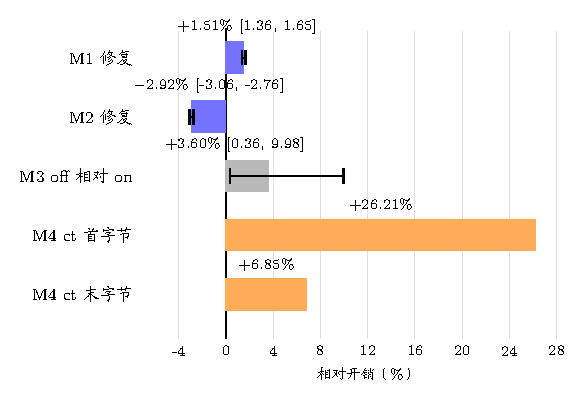
\includegraphics[width=0.92\textwidth]{assets/fig7.pdf}
\caption{防护前后成对相对开销}
\label{fig:overhead}
\par\smallskip
{\footnotesize 图注：M1 +1.51\%，M2 $-2.92\%$，M4 小内核 +26.21\%/+6.85\%。M3 的区间宽，只作描述；M4 是 32 B 比较调用，绝对差只有数纳秒，不能外推到完整解封装。}
\end{figure}

开销测量不是“前后各跑一次”。decaps 每臂 6 块 $\times$ 25,000 次，keygen 与 encaps 各 30,000 次，两臂按 ABAB 交错，相对开销用 bootstrap 10,000 次给区间。交错是为了让频率漂移、缓存状态与后台服务的影响同时落在两臂上；分块是为了让每块内部的顺序随机化。一次“修复前跑一遍、修复后跑一遍”的差值，无法区分防护开销与环境漂移。

M1 的 +1.51\% 可以拆成“多出的指令”与“多出的调用”。掩码选择把一条分支换成置位、取负、异或、与、再异或，指令数增加几条；16 位条件传送辅助函数在 -Os 下没有内联，多一次调用与返回。两部分加起来是 862.6 ns，占 57,010.7 ns 的 1.51\%。这个拆法只作解释，不作为精确归因；指令级开销要看反汇编与微基准。% A-25

M1 的 +1.51\% 是四次测量中最稳定的一个：区间窄，方向单一，与掩码选择多出的几条指令相符。M2 的修复反而更快，M3 的区间很宽，M4 的相对值很大但绝对差很小；三个对象的解释分别落在下面三段。

M2 的负开销来自编译器。除法被乘法与移位替代后，指令数减少，流水线停顿也减少；修复版反而比未修版快 2.92\%。这不等于“修复更安全”，只说明“更安全”与“更快”可以同向，也可以反向。把负开销写成“优化”会偏离主题：本作品测的是防护开销，不是性能优化。

M3 的 +3.60\% 区间 [0.36, 9.98] 很宽，是因为 off 臂的方差大、样本块少；这个区间只作描述，不用它推断总体开销。M3 是人工夹具，on/off 两臂只差一张查表；查表的开销在完整解封装里占比很小，测量噪声容易淹没它。把 3.60\% 写成“查表的开销”会高估精度。

M4 的 +26.21\% 与 +6.85\% 是相对值，绝对差只有 4 ns 量级。首字节与末字节的差异不同，是因为比较提前返回的位置不同：vulnerable 臂在第一个字节不同时最快返回，在最后一个字节不同时最慢；ct 臂始终遍历全部字节。两个百分比不能平均，也不能与完整解封装的百分比比较。

把相对开销换算成绝对时间：M1 每解封装多 862.6 ns，M2 少 1,690.5 ns；M3 的 +3.60\% 按 29,455.7 ns 的参考均值换算约 1.06 $\mu$s，但区间跨到 9.98\%，绝对量的不确定性也很大；M4 的 +26.21\% 只在小内核的比较调用上成立。绝对量与相对量一起看，才能判断这个开销在实际使用中的位置。% A-25 % B-02

M1 的 +1.51% 与 M2 的 −2.92% 方向相反，说明“防护一定变慢”不成立。掩码选择多出指令，除法替代减少指令；两个修复对指令数的影响不同，开销的方向也不同。把这两个数放在同一张图上，是为了让读者看到方向，而不是为了比较大小；不同对象的百分比不能直接排序。

M4 的 +26.21% 与 +6.85% 只用于说明“小内核的相对开销可以很大”。32 B 比较的基线远小于完整解封装，多几条指令就会带来 26% 的相对变化；换成 57 $\mu$s 的完整解封装，同样的指令数只占 0.0x%。相对开销必须绑定基线，脱离基线比较百分比没有意义。

开销的置信区间来自 bootstrap，不来自正态假设。M1 的区间 [1.36, 1.65] 窄，说明 6 块 $\times$ 25,000 次的成对测量稳定；M3 的区间 [0.36, 9.98] 宽，说明 off 臂的方差大、块数少。区间宽时只作描述，不用它推断总体；区间窄时也不把点估计当成精确值，只说明这次测量的相对开销落在那个范围。

表~\ref{tab:runtime} 同时给均值与分位数，是为了让读者看到分布的形状。均值对长尾敏感，分位数对长尾稳健；两者相差不大时，均值可以作为摘要；相差大时，分位数更能代表典型调用。这批数据的均值与中位数相差不到 100 ns，说明分布没有被长尾拉偏；如果只给均值，读者无法判断这一点。% A-25

性能开销不是本作品的目标，防护效果才是。开销测量的作用是回答“防护的代价有多大”，不是“哪个实现更快”；把 M2 的 $-2.92\%$ 写成“性能优化”会偏离主题。报告给开销区间，是为了让读者判断这个代价是否可以接受，而不是为了给实现排名。

五个对象的行不是同一把尺子。M1 与 M2 是完整解封装，可以互相比均值；M5 也是完整解封装，但实现不同，均值的差异主要来自参考路径，不来自防护；M3 与 M4 是小内核，只用于相对开销，不进入这张表。表~\ref{tab:runtime} 只列能放在同一窗口里比较的对象，跨对象的均值差不在结论里。

周期列只用于跨机器粗略对齐。周期按名义 4.30 GHz 换算，而实测频率中位数是 4,309,722.5 kHz，偏差 +0.005\%；用名义频率换算会带来同量级的系统误差。周期列不写进结论，也不与别的机器比较指令数；它只是让读者对“57 µs 在 4.30 GHz 下大约是多少个周期”有个量级概念。% A-31 % B-02

keygen 与 encaps 也做了测量，各 30,000 次，但表~\ref{tab:runtime} 只列 decaps。decaps 是防护的主要对象：M1 的分支、M2 的除法、M3 的查表、M4 的比较都在解封装路径上；keygen 与 encaps 的防护开销不是本轮重点。把 decaps 的开销写成“整个 KEM 的开销”会夸大适用范围。

开销测量与功能测试使用同一份产物；换构建要重测，这条约束与产物绑定一致。成对分块与 ABAB 交错解决的是“环境漂移”与“顺序效应”。如果先跑未修臂再跑已修臂，频率漂移、缓存升温与后台服务变化都会落在已修臂上；ABAB 让两臂在时间上交错，漂移同时落在两臂上。bootstrap 10,000 次给区间，不假设正态；区间窄说明相对开销稳定，不说明绝对耗时稳定。

表~\ref{tab:runtime} 的均值与图~\ref{fig:overhead} 的相对开销要一起读。均值给绝对量级，相对开销给可比的比例；只看均值，M1 与 M2 的差异只有 862.6 ns，容易被当成噪声；只看比例，+1.51\% 又缺少绝对量级。两者并排，读者才能判断“这个开销在 57 $\mu$s 里占多少”。% A-25 % B-02

表~\ref{tab:runtime} 与图~\ref{fig:overhead} 证明防护在本机带来的实测开销，以及成对设计能把环境漂移压到区间里；它们不证明开销低就一定安全，也不证明开销高就一定泄漏。M2 修复更快，不能写成“更安全”；M4 的百分比不能与完整解封装的百分比直接比较。

\subsection{编译选项与测量条件}
% A-26 优化级别 12 格
% A-29 锁频对照
% A-30 计时精度
% A-32 WSL2 复现
% B-11 优化矩阵

同一份源码在不同优化级别与测量条件下会呈现不同的产物形态与可检出性；结论必须绑定编译条件。图~\ref{fig:opt} 给出 12 格的合并均值差与 95\% 区间：M1 两版与 M5 各四个优化级别。% A-26 % B-11

\begin{figure}[htbp]
\centering
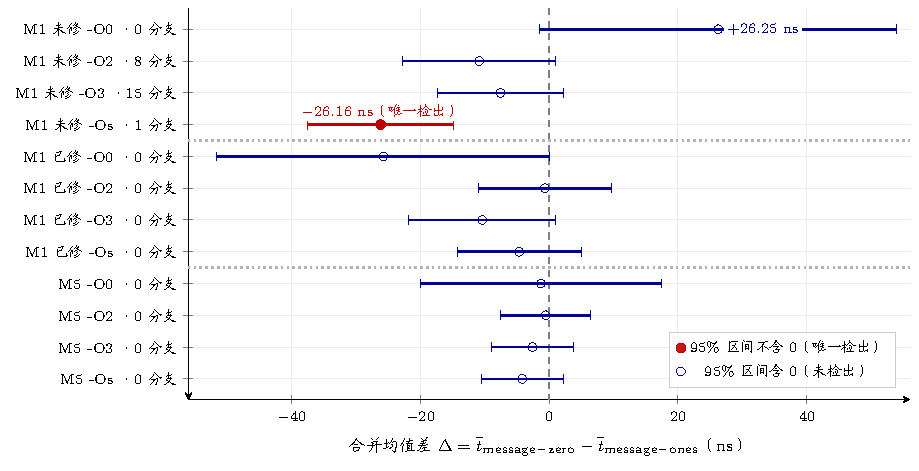
\includegraphics[width=0.98\textwidth]{assets/fig8.pdf}
\caption{优化级别 12 格合并均值差与 95\% 区间}
\label{fig:opt}
\par\smallskip
{\footnotesize 图注：只有 M1 未修 -Os 格区间不含 0；-O2/-O3 分支更多但计时未检出。区间为三个种子的逆方差合并；同一格三个种子使用同一份二进制。}
\end{figure}

12 格来自 3 个臂 $\times$ 4 个级别。3 个臂是 M1 未修、M1 已修与 M5；4 个级别是 -O0、-O2、-O3、-Os。每个格做产物判定（反汇编、除法计数、Memcheck）与锁频计时（每格 3 个种子），两列证据分开登记。

把产物判定与计时判定分开，是为了避免“分支存在但计时没测到”被读成“分支不存在”；-O2 与 -O3 正是这种情况。每格三个种子的二进制摘要逐字相同，判定用的产物与计时用的产物对齐；这一条是 12 格可比的前提；换优化级别或编译器都要重新登记产物，这条约束不随环境改变。

12 格是族外探索，不进任何 Holm 家族。它的作用是看“产物形态与可检出性是否随编译条件变化”，不是给每个优化级别下安全结论；每格 3 个种子，样本量不足以做家族检验，也不足以估计总体。结论止于“该级别下没有观察到可区分差异”。

M1 未修的 -Os 格合并 $-26.16$ ns，区间 [$-37.51$, $-14.81$]，是 12 格中唯一不含 0 的区间；同一版本的 -O2 与 -O3 分别合并 $-10.86$ 与 $-7.55$ ns，区间都含 0；-O0 没有秘密相关分支，源码的算术掩码被原样保留。产物侧，-O2 与 -O3 的秘密相关分支位置数为 8 与 15，比 -Os 的 1 个更多；分支更多，计时反而未检出。修复版四个级别都是 0 个秘密相关分支，M5 四个级别都是 0，12 格都没有整数除法指令。% A-26

其余 11 格的区间同样列出。M1 未修 -O0 合并 +26.25 ns，区间 [$-1.42$, 53.92]；-O2 $-10.86$ [$-22.75$, 1.02]；-O3 $-7.55$ [$-17.35$, 2.26]。M1 已修 -O0 合并 $-25.75$ [$-51.59$, 0.09]，上界紧贴 0；-O2 $-0.69$ [$-11.02$, 9.63]；-O3 $-10.38$ [$-21.77$, 1.00]；-Os $-4.64$ [$-14.29$, 5.02]。

M5 四格都在 $-5$ ns 以内，区间都含 0。只有 -Os 未修格的距离离 0 足够远。

“分支更多反而未检出”有两层解释。产物层：-O2/-O3 的每比特测试是“内存操作数加条件跳转”，形态与 -Os 的寄存器位测试不同；分支数量多，不等于单条分支的代价大。计时层：分支的代价被流水线、分支预测与乱序执行吸收，端到端均值差可能小于 MDE；-O2/-O3 的区间都含 0，说明这个预算下没有分辨出来。两层解释都指向同一个结论：不能从“分支数量”推断“可检出性”。

锁频与不锁频的对照给出另一个反直觉结果。三个对象的 CV 比为 0.964、1.006、1.089，SD 比为 0.741、0.757、0.956；不锁频的标准差反而更低。M1 未修在两种条件下都是 3/3 检出，M5 都是 0/3；判定一致，稳定性指标的方向却不一致。% A-29

CV 比的方向不一致，说明“锁频降噪”这个直觉在这台机器上不成立：M1 未修 0.964、M1 已修 1.006 小于或等于 1，M5 1.089 大于 1；如果锁频一定降噪，三个比值应该都大于 1。SD 比都小于 1，是因为不锁频时频率更高、单次调用更短，绝对标准差随均值一起缩小；换成 CV 后，两者的相对离散度接近。锁频真正提供的是可核对的工作点：每次运行记录 20 次探针、退出核对恢复，审计者能确认“这次采集在什么频率下完成”。

-O0 格没有秘密相关分支，是“该级别下这个机制没有出现”，不是“这份源码安全”。源码的算术掩码被原样保留，编译器没有把它还原成条件跳转；换一个编译器或换一个 -march，-O0 也可能出现分支。把 -O0 的 0/0 写成“最安全的级别”会越过产物边界；本作品只写“该级别下没有观察到该机制”。

修复版四个级别都是 0 个秘密相关分支，说明官方修复在不同优化级别上都生效；它不说明修复版在计时层也不可区分。M1 已修的四个级别合并值分别为 $-25.75$、$-0.69$、$-10.38$、$-4.64$ ns，区间都含 0；这是产物层与计时层分开登记的结果。产物层 0 个分支、计时层区间含 0，两者同向，但不能互相替代。

三台 WSL2 虚拟化环境的复现把“机制”和“可检出性”分开。确定性证据与主平台一致：M1 未修 -Os 1 个、-O2 8 个、-O3 15 个、-O0 0 个 Memcheck 上下文，修复版与 M5 全为 0，反汇编形态逐项相同。时间证据不同：三台机器上 M1 未修 -Os 的合并区间都含 0，M4 vulnerable 的合并区间都不含 0（$-7.13$、$-11.97$、$-22.37$ ns）。机制存在与否可以跨环境复现，数十纳秒效应的可检出性依赖测量环境；WSL2 数据不进任何 Holm 家族，也不与裸金属数据合并。% A-32

WSL2 的三台机器不是三台测量机。它们是虚拟化环境，不锁频，时间数据的标准误在数百纳秒；三台机器的一致之处是确定性证据（反汇编、Memcheck），不是时间证据。M4 vulnerable 在三台机器上都给出不含 0 的区间，说明管线在效应足够大时仍能检出；M1 未修 -Os 的区间都含 0，说明 32 ns 效应在虚拟化噪声下不可检出。

WSL2 的结果还说明“效应足够大时管线仍能检出”。M4 的 4 ns 效应在虚拟化噪声下仍能给出不含 0 的区间，是因为比较调用的方差小、信噪比高；M1 的 32 ns 效应在 WSL2 上反而测不到，是因为完整解封装的方差大、虚拟化噪声高。可检出性不是只由效应绝对值决定，还由噪声与样本量决定；同一台机器上，M4 的 MDE 比 M1 小两个数量级，原因就在这里。

计时精度决定了什么样的效应可以被讨论。读钟开销约 17.4 ns，最小步进 10 ns；时间戳计数器的速率为 4,291,962 kHz，单次读数的分辨率下界为 42--43 个计数、约 9.8--10.0 ns；1 ms 短区间的频率极差为 348 kHz，相对标准差 $5.4\times10^{-6}$。逐调用物理恒频不可主张：锁频协议固定的是工作点，不是每一次调用的频率。% A-30

时间戳计数器的读数不是物理时间的直接测量。TSC 速率 4,291,962 kHz 是按名义频率校准的；单次读数 42--43 个计数对应 9.8--10.0 ns，是分辨率下界，不是精度。1 ms 短区间的频率极差 348 kHz、相对标准差 $5.4\times10^{-6}$，说明短窗内频率稳定；长期稳定性没有认证，逐调用物理恒频不可主张。

锁频/不锁频对照每组只有 3 次运行，只作描述。3 次运行不足以估计总体方差，也不足以推断其他处理器或调速策略；CV 比 0.964--1.089 只能说明“这台机器上方向不一致”，不能说明“锁频在所有机器上都不降噪”。把这条对照写成普遍结论，会超出样本边界。

图~\ref{fig:opt} 与这组对照证明产物与测量条件会改变可检出性；它们不证明某个优化级别绝对安全，也不证明其他编译器、其他 CPU 会给出同样的结果。本机未配置 isolcpus，SMT 开启，后台约 39 个服务在运行；这些条件与 10 ns 量化一起，构成时间证据的环境边界。

\subsection{架构与网络边界}
% A-27 aarch64 12 格
% A-28 同机网络五档
% A-30 计时精度
% B-03 检测预算
% B-12 网络档位

M1 的泄漏机制是 x86\_64 特定的编译器产物；同机网络各档在本预算下未检出，不能外推真实远程。图~\ref{fig:boundary} 把架构对照与网络检测预算放在一起：左侧是同一份源码在两个架构上的产物形态，右侧是五档网络分辨同一量级效应所需的样本数。% A-27 % A-28

aarch64 的实验条件是“真指令集、原生二进制”。它在 Apple Silicon 的容器内运行，运行时报告的机器类型是 aarch64，不是 QEMU 翻译，也不是交叉编译后在 x86\_64 上跑；同一份 liboqs 0.10.0 源码、同一个 clang 18、同一组优化级别，只换架构。这个条件让“产物形态不同”可以归因到架构，而不是源码或编译器版本。

容器环境的限制要写明：没有锁频，没有裸金属，CPU 与其他容器共享；这些条件不影响确定性证据（反汇编、Memcheck），但影响时间证据。aarch64 的 12 格只做产物判定与 Memcheck，不做锁频计时；把它的时间数据与 x86\_64 合并会引入不可控的环境差异。

\begin{figure}[htbp]
\centering
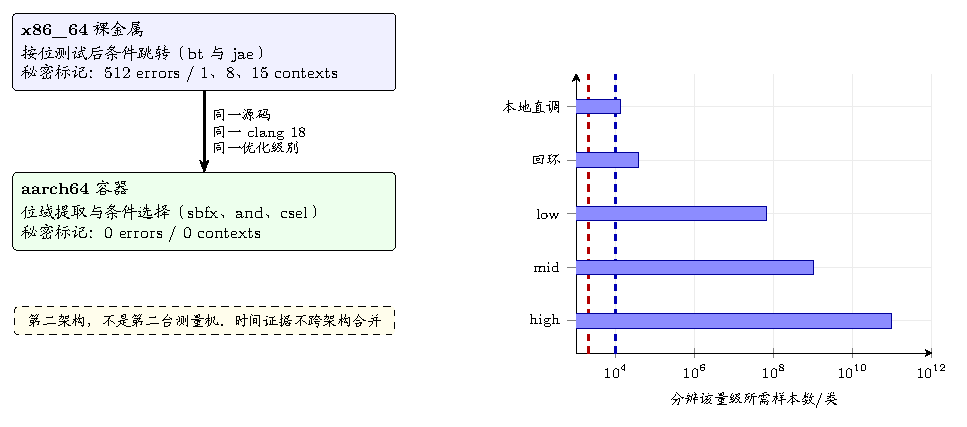
\includegraphics[width=0.99\textwidth]{assets/fig9.pdf}
\caption{架构与网络边界}
\label{fig:boundary}
\par\smallskip
{\footnotesize 图注：x86\_64 的 bt/jae 在 aarch64 上变为 sbfx/csel；网络各档在本预算下未检出。右侧虚线为本轮实际样本数（网络每类 2,000，本地直调每类 10,000）。}
\end{figure}

aarch64 的 12 格全部是 0 errors / 0 contexts；x86\_64 同格的 M1 未修是 512 errors / 8、15、1 个上下文。反汇编上，x86\_64 是按位测试后条件跳转（bt 与 jae），aarch64 是位域提取、与掩码、条件选择（sbfx、and、csel），消息位的选择全部走无分支算术。同一份源码、同一个 clang 18、同一个优化级别，产物性质不同；M1 的机制不是“ML-KEM 参考实现在别的架构上也泄漏”，而是 x86\_64 编译器在特定选项下的产物。

x86\_64 的 512 errors / 8、15、1 个上下文，对应 -O2、-O3、-Os 三个级别；aarch64 同格都是 0/0。-O0 在两个架构上都是 0，因为源码的算术掩码被原样保留。三个不一致的格子全部落在“x86\_64 加 M1 未修”，这个分布说明差异绑定的是架构与产物的组合，不是探针或输入。

12 格里 9 格一致、3 格不一致，不一致的全部集中在 x86\_64 的 M1 未修臂。这个分布本身就是证据：如果差异来自探针或环境，应该在各臂上随机出现；差异只在“x86\_64 加 M1 未修”这一组出现，说明它绑定的是产物形态，不是测量环境。aarch64 上消息位选择走无分支算术，Memcheck 没有秘密相关分支可报，0/0 是产物性质的结果。

aarch64 上 0/0 的原因可以直接从反汇编读出来：消息位的选择走位域提取、与掩码、条件选择，三个步骤都不产生依赖秘密的跳转；Memcheck 没有秘密条件跳转可报，也没有秘密下标可报。0/0 不是“工具没跑”或“输入没覆盖”，而是“产物里没有这个机制”；同一份探针在 x86\_64 上报 512 errors，说明探针本身有效。

aarch64 跑在容器内，未锁频，不是裸金属；它只构成第二架构，不是第二台测量机。跨架构的时间证据不合并，也不要求同号；两个架构的探针实现不完全相同，M5 的跨架构结论只能由“两架构都是 0”弱支撑，不能写成强结论。把 aarch64 写成“第二台测量机”会夸大证据：它没有锁频，没有裸金属，时间数据不进入任何家族。

两个架构的探针实现不完全相同：x86\_64 的 M5 四格用另一个探针，aarch64 用同一份历史探针；M5 的跨架构结论只能由“两架构都是 0”弱支撑。两架构都是 0 只支持“未检出”；探针不同，不能升级为常数时间结论。

同机网络场景用裸金属、匿名网络命名空间、自有 veth 与内核 netem 构造两端 TCP，分五档：本地直调、回环、low、mid、high。本地直调档 M1 未修两次运行一次可分辨（+37.1 ns，区间 [20.4, 53.8]）、一次未检出（$-7.9$ ns，区间 [$-25.0$, 9.2]）；网络各档全部未检出。分辨同一量级效应所需的每类样本数为 13,098、38,417、64,636,555、1,003,153,317、97,586,175,893；网络各档实际每类 2,000，比所需少 1.3--7.7 个数量级。% B-03 % B-12

网络拓扑是同机两端：服务端在匿名 netns 内，绑到锁频 CPU2；客户端在宿主 netns，绑到 CPU0/1/3，不占 CPU2/CPU6。veth 两端用一对私有 /30 地址；netem 挂在 veth 两端，单向延迟与抖动分别是 100 $\mu$s/20 $\mu$s、1 ms/200 $\mu$s、10 ms/2 ms。这个拓扑能加入协议栈、排队与链路抖动，不能加入真实广域网的拥塞与路由变化。

网络五档的设计是为了分离“协议栈”“排队”与“链路抖动”三项开销。本地直调不走 socket，回环走 veth 与 TCP 但不加 netem，low/mid/high 逐级加入延迟与抖动；五档的检测预算逐级上升，说明每加入一层开销，分辨同一效应所需的样本数就增加。这个阶梯是定性的，不是对真实网络的拟合。

本地直调档的两次运行给出了两种结果：一次 +37.1 ns、区间 [20.4, 53.8]，一次 $-7.9$ ns、区间 [$-25.0$, 9.2]。两次的噪声水平接近，差别来自效应本身的运行间变动；把两次合并得到的参照效应区间含 0，只能当量级参照。这段结果说明：即使在同一台机器、同一锁频工作点，32 ns 级效应的可分辨性也不是每次都稳定；网络档每类只有 2,000，更不可能稳定分辨。

网络档的 netem 参数是单向 100 µs/20 µs、1 ms/200 µs、10 ms/2 ms，三档对应 low、mid、high。回环档不走 netem，只有 veth 与 TCP 的开销；本地直调档不走 socket，直接调用解封装。五档的设计是为了让“协议栈与排队”逐级加入，而不是一步跳到真实远程。即使最轻的回环档，所需样本数也比实际多 1.3 个数量级；加上 netem 后，所需样本数上升到 $10^7$--$10^{11}$，实际每类 2,000 远远不够。

检测预算按 $n=2(1.96\,\mathrm{SD}/|\Delta|)^2$ 计算，与 MDE 同口径；本地直调 13,098、回环 38,417、low 64,636,555、mid 1,003,153,317、high 97,586,175,893。网络各档实际每类 2,000，回环差 1.3 个数量级、low 差 4.5 个、mid 差 5.7 个、high 差 7.7 个。预算数字不是“需要这么多才能攻击”，是“需要这么多才能分辨这个量级的差异”；两者不能混。

网络档每类 2,000 的样本量是预算与机时的折中。按本地直调的 13,098 所需样本，2,000 只有 0.15 倍；按 high 档的 97,586,175,893，2,000 差 7.7 个数量级。样本量不足时，未检出是预期结果，不是“网络没有泄漏”的证据；报告把预算与差距一起写出，是为了让读者自己判断这个阴性有多强。

netem 的三档不是“轻度、中度、重度网络”的通用定义，是本作品选的三组参数。low 档 100 $\mu$s/20 $\mu$s 接近同城链路，mid 档 1 ms/200 $\mu$s 接近跨城，high 档 10 ms/2 ms 接近跨洲；这些类比只用于读者建立量级感，不是真实测量。真实远程的排队、拥塞与路由变化不在这个拓扑里。

这是同机模拟，不是真实远程；网络各档的“未检出”只说明在本预算下没有看到可区分差异，不说明远程链路上不存在泄漏，也不说明远程攻击不可行。图~\ref{fig:boundary} 证明机制与可检出性有环境边界；它不证明远程攻击可行或不可行，也不证明某个架构绝对安全。在同机模拟里，网络各档的检测预算比实际样本高 1.3--7.7 个数量级；在真实远程里，链路抖动、拥塞与路由变化只会让预算更高，不会更低。这个方向性判断不依赖具体数字，但它是推断，不是实测；本作品不把它写成“远程不可测”。

\subsection{多工具交叉验证}
% A-16 RTLF
% A-24 工具矩阵
% B-04 RTLF 数据集
% B-05 工具矩阵分解

单工具会给出方向相反的读法；交叉矩阵的价值不是“工具多”，而是让每个工具的“回答什么、不回答什么”落在同一张表上。图~\ref{fig:tools} 是 9 工具 $\times$ 5 模块的矩阵：30 格有真实运行产物，15 格未运行。% A-24 % B-05

\begin{figure}[htbp]
\centering
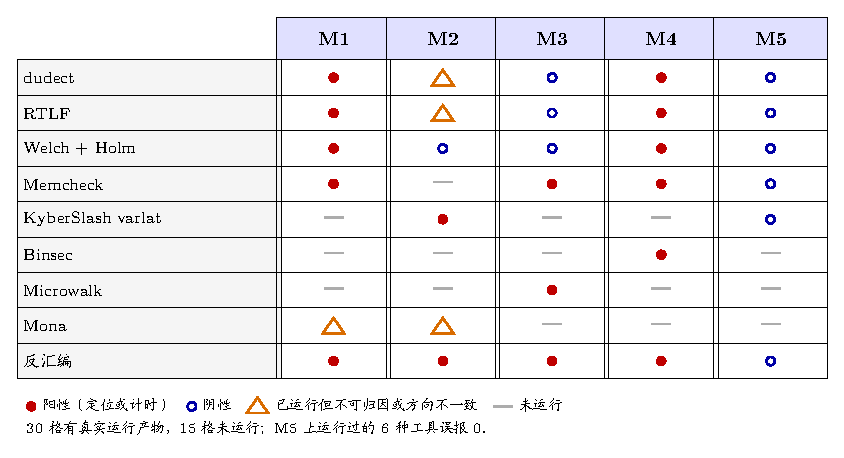
\includegraphics[width=0.96\textwidth]{assets/fig10.pdf}
\caption{多工具交叉矩阵}
\label{fig:tools}
\par\smallskip
{\footnotesize 图注：30 格有真实产物，15 格未运行；M5 上 6 工具误报 0。阳性指该工具在其判定层报告了机制或可区分性，阴性指未报告；未运行不等于阴性。}
\end{figure}

矩阵的 9 个工具分三类：族内统计（Welch+Holm）、族外统计（dudect、RTLF、Mona）、定位工具（反汇编、Memcheck、varlat、Microwalk、Binsec）。三类回答的问题不同，矩阵把它们放在同一组模块上，是为了看“同一对象在不同判据下会不会给出相反读法”。15 个未运行格都写了原因：M2 没有完整解封装的 Memcheck 探针，M1/M2 没有 Binsec 抽取内核，M3/M4/M5 没有接入 Microwalk，Mona 只接入 M1/M2。未运行格不填阴性。矩阵按 2026-10-16 冻结的产物登记；M5 上的有界验证结果在矩阵冻结后补充，列在 3.4，不计入这张矩阵的 30 格与 6 工具统计。矩阵的格数不随补充结果改变；未运行格也不因补充结果改填阴性。

三类工具的回答范围不同。族内统计回答“均值差是否可区分”，族外统计回答“分布是否不同”，定位工具回答“哪里依赖秘密”。同一格在族内统计是阴性、在族外统计是阳性，不是矛盾：它们比较的对象不同。矩阵把三类放在一起，是为了让读者看到“同一对象在不同判据下可以给出不同读法”，而不是让它们投票。

M1 是五路同向的例子：反汇编看到按位测试后条件跳转，Memcheck 看到 1 个秘密条件跳转，Welch+Holm 拒绝主类对，RTLF 在未修臂报告差异、在已修臂未报告，dudect 最大 $t$ 在未修臂为 26.41、40.64、14.92、在已修臂为 1.15、1.12、1.31。五类工具回答的问题不同，结论同向。

五路同向增加信心，但不等于“五倍证据”：它们共享同一份产物与同一组输入，不是五个独立实验。

M4 是人工夹具中唯一定位层与计时层都阳性、ct 臂全阴性的正对照。M5 上运行过的 6 种工具全部阴性，误报 0；这个数字只说明这 6 种工具在这个对象、这些输入上没有报假阳性，不能估计总体误报率。

M4 的正对照作用是把“定位阳性”与“计时阳性”同时钉在一个对象上。如果 M4 的 ct 臂也阳性，说明检测链路有假阳性；如果 vulnerable 臂阴性，说明链路测不到已知机制。两种失败都没有出现，M4 才能作为正对照。M5 的阴性对照作用相反：如果 6 种工具在 M5 上报阳性，说明工具有误报；6 种都报 0，说明本次没有误报。

误报 0 的分母是 6 个工具 $\times$ 1 个对象，不是 6 个工具 $\times$ 全部输入。M5 上每种工具只跑了一组输入或一个探针；换一组输入、换一个优化级别，误报率可能不同。把“6 工具误报 0”写成“工具不会误报”会越过样本边界；写成“本次未出现误报”才是准确的。

单工具误读在 M2 上最清楚。只看 RTLF，会把 M2 读成“两臂都可区分”：主类对 6/6 检出，未修与已修各 3 次；只看 dudect，会因阳性落在已修臂（36.27、30.94、61.91 对 4.68、3.05、3.66）而得出“修复引入泄漏”。两个读法都与端到端 Welch 检验的未检出冲突。\cite{dudect}

Mona 的不一致原样保留。M1 未修臂全部无分离、已修臂 2/6 次分离，与 Welch、RTLF、dudect 的方向都不一致；它的“置信”字段是批次成功百分比，不是 $p$ 值，不能参与 Holm，也不能用来推翻既有结论。把 Mona 的不一致写成“工具有问题”或“结论有问题”都越界；它只说明这个工具的判据与另外三类不同。

M2 的两个误读来自不同的判据。RTLF 比较分布与分位，主类对使消息位走系统性不同的路径，分布差异可能来自分支而不是除法；dudect 用在线 $t$ 检验，阳性落在已修臂，说明它测到的是修复引入的另一种差异，不是除法。两个工具都没有定位到除法热点；把它们与 Memcheck、varlat 的定位结论交叉，才能得到“定位阳性、计时未检出”的完整读法。

15 个未运行格分布在 5 个工具上：Memcheck 缺 M2 的完整解封装探针，varlat 缺 M1/M3/M4，Binsec 缺 M1/M2/M3/M5，Microwalk 缺 M1/M2/M4/M5，Mona 缺 M3/M4/M5。每一格都写了原因；补上它们需要额外的探针、抽取内核或工具接入。未运行格不是阴性，也不是“无关紧要”；它们只是本轮没有数据。

图~\ref{fig:tools} 证明多工具交叉能消除单工具误读，并把“未运行”与“阴性”分开；它不证明所有工具都同意，也不证明没有假阴性。15 格未运行不等于阴性，未运行格只写原因，不填结论。补上这些格需要额外的工具安装与模型构建，本作品没有做。

交叉矩阵不产生新的统计判定。它把已有工具的结论放在同一张表上，让读者看到“同一对象在不同判据下可以给出不同读法”；它不做投票，也不把多数工具的意见当成结论。主结论仍由预注册 Holm 家族给出，矩阵只负责解释与边界。

\subsection{可复现性}
% A-37 干净 clone 与匿名包
% B-09 测试总数

可复现不是“代码在仓库”，而是“干净 clone 能跑、包内能复算、每个数字能回到原始行”。一键入口分 quick 与 full 两档：quick 不写 sysfs、不绑核，用固定输入跑功能与统计复算；full 需要锁频控制器与裸金属硬件，按冻结计划重采时间数据。

quick 档的设计目标是“在任何一台能编译的机器上跑通软件流程”。它不写 sysfs，不需要 root，不绑核；它跑功能测试、统计重算与报告生成，不产生新的时间结论。full 档才需要锁频控制器、裸金属与固定的 CPU；它按冻结计划重采，产出原始长表与运行台账。两档分开，是为了让“软件流程可复现”与“时间结论可复现”不混为一谈：前者任何机器都能做，后者需要硬件。

quick 档的输入是固定的，输出是功能测试结果与统计重算结果；它不产生新的时间数据，因此不需要锁频。full 档的输入是冻结计划，输出是原始长表与运行台账；它需要锁频控制器、绑核与恢复核对。两档的入口是同一个脚本，参数不同；把两档分开，是为了让读者知道“跑通”与“复现时间结论”是两件事。

干净 clone 的四个测试集合计 263 项通过、0 失败：platform 88、ordinary 57、sanitize 57、historical-fixed 61。匿名包解出后 CTest 5/5。随包提供 42 份原始长表、逐次运行台账、冻结计划、产物摘要与统计脚本；每个正文数字可以按附录 B 的运行编号回到原始行，统计判定可以按附录 C 的公式与脚本复算。% A-37 % B-09

42 份原始长表是逐次运行的原始值，不是汇总表；每份长表带运行编号、模块、臂、种子、CPU 与产物摘要。逐次运行台账记录每次控制器运行的进入、采中、退出三段；冻结计划记录主类对、样本量、停止条件与 Holm 家族；统计脚本按附录 C 的公式重算。四类材料合起来，第三方可以从原始值走到正文数字。

263 项测试是软件流程验证，不是计时复现。platform 88 项覆盖平台自身的构建与接口，ordinary 57 项覆盖普通构建，sanitize 57 项覆盖 ASan/UBSan 构建，historical-fixed 61 项覆盖历史修复版；四类合起来说明代码在各构建配置下能跑、功能测试能过，不说明时间结论能在别的机器上复现。263 项证明的是流程，不是时间。

复现边界要写清楚：完整锁频采集需要硬件，包内不能代替；外部 RTLF、Mona、dudect、Binsec 不在包内重跑，只保留输出摘要与调用参数；包内复算只重算已有数据，不产生新实验。这组结果证明软件流程与统计判定可复算，不证明任何机器都能复现时间结论；时间结论依赖本机、本编译产物与锁频工作点。

匿名包解出后 CTest 5/5，是包内复算的入口。它验证包内构建、功能测试与统计脚本能在干净环境里跑通；它不重跑外部工具，也不重采时间数据。5/5 说明包内流程可复算，不覆盖外部工具与时间数据。

\clearpage
% 第 4 章 与现有工作对比及应用前景
% 本章引用键（实际使用）：tvla, dudect, rtlf, ctgrind, microwalk, kyberslash, ctverif, binsec, clangover, azouaoui2021, jancar2022
% 表号接第 3 章（表 6–11），本章从表 12 起；本章不放图
\setcounter{table}{11}

\section{与现有工作对比及应用前景}

\subsection{泄漏检测与评估方法对比}

软件时间侧信道的评估分为三条路线：统计检测、动态分析与形式化验证。本作品不提出新的检测原语，贡献在于把三条路线组织进同一个以产物为中心、可审计的流程。第 2 章讲这套流程怎么搭，本章讲它与既有路线各自回答什么问题、答案能用到哪一步。

统计检测把程序当黑盒。TVLA\cite{tvla} 比较固定类与随机类的轨迹分布，dudect\cite{dudect} 把同一判据搬到在线计时，用最大 $t$ 与上游阈值给二值结论，RTLF\cite{rtlf} 比较分布与分位，并用 bootstrap 控制第一类错误。三者都只回答“两类样本能不能分开”，不回答差异来自哪条指令；类对构造、样本顺序与运行间漂移都会改变结论。第 3.12 节的 M2 是一个现成例子：RTLF 读成两臂都可区分，dudect 的阳性落在已修臂，预注册的均值检验却两个臂都未拒绝。

动态分析在程序内部找秘密依赖。ctgrind 沿用 Valgrind 的秘密标记，报告秘密进入分支条件或访存下标的时刻\cite{ctgrind}；Microwalk 用执行轨迹与互信息找与秘密关联最强的指令\cite{microwalk}；varlat 检查除法一类可变时延指令的操作数是否含秘密\cite{kyberslash}。这类工具能给出函数级甚至指令级的落点，但只覆盖实际执行过的输入，也不回答“这台机器上能不能测到”。定位阳性与计时阳性是两件事，M2 的三处除法正是两者分离的例子（第 3.4 节、第 3.7 节）。

形式化验证在给定模型与边界内给出另一种结论：证明控制流与访存不依赖秘密。ct-verif 把常数时间归结为产品程序的安全性，在中间表示层完成这类证明\cite{ctverif}；Binsec/Rel 用关系符号执行在二进制层做有界检查，并给出反例路径\cite{binsec}。它们的成本高，通常不建模指令时延、缓存与流水线，所以能回答“是否依赖秘密”，不能回答“本机计时是否可区分”。第 3.4 节 M4 的不安全判定与 ct 臂的有界安全、M5 的 1088/1088 路径完成，都属于有界结论。

表~\ref{tab:compare} 把三条路线与本作品的定位放在同一组维度上。每一行的最后一列写出这个差异导致的实践后果，而不只是一个勾。

\begin{table}[H]
\centering
\caption{泄漏检测与评估方法对比}
\label{tab:compare}
{\footnotesize
\begin{tabularx}{\textwidth}{|>{\raggedright\arraybackslash}p{2.7cm}|>{\raggedright\arraybackslash}p{2.3cm}|>{\raggedright\arraybackslash}p{2.3cm}|>{\raggedright\arraybackslash}p{2.5cm}|>{\raggedright\arraybackslash}p{2.3cm}|>{\raggedright\arraybackslash}X|}
\hline
方法 & 本机可测性 & 函数级定位 & 产物级证明 & 未检出的量化 & 多机制/防护复测 \\
\hline
TVLA\cite{tvla}、dudect\cite{dudect} & 是（黑盒计时） & 否 & 否 & 一般不报，阴性无预算 & 需另行组织；后果：换产物要整体重判 \\
\hline
RTLF\cite{rtlf} & 是（第一类错误有界） & 否 & 否 & 随样本量提高功效，不报 MDE & 需另行组织；后果：分布差异无法归因到指令 \\
\hline
ctgrind\cite{ctgrind}、Microwalk\cite{microwalk} & 否（不回答本机可测性） & 是（分支、访存、轨迹） & 否 & 不适用（只报依赖） & 单一机制类；后果：定位阳性易被读成可利用 \\
\hline
varlat\cite{kyberslash} & 否 & 是（除法等可变时延指令） & 否 & 不适用 & 针对单一指令类；后果：只覆盖已知机制，漏掉新形态 \\
\hline
ct-verif\cite{ctverif}、Binsec/Rel\cite{binsec} & 否 & 是（函数或内核） & 是（给定边界内；ct-verif 在中间表示层） & 不适用（二值结论） & 单一函数或内核；后果：不建模指令时延，答不了本机计时 \\
\hline
本作品（A-16、A-24、A-26、A-27） & 是（预注册 + Holm + MDE） & 是（多工具交叉） & 部分（M4、M5 有界） & 报告 MDE 与样本量 & 5 模块统一规程、防护前后同规程复测；后果：结论绑定产物、可按层追溯 \\
\hline
\end{tabularx}
\par\smallskip
{\footnotesize \textbf{表注：}三条路线回答不同问题：统计检测判“是否可区分”，动态分析判“哪里依赖秘密”，形式化判“给定边界内是否常数时间”。本作品不改变这些判据，只把三类证据登记在同一产物上；“部分”指 M4、M5 的有界验证，不是全实现认证。}
}
\end{table}

五列维度各有用途。本机可测性决定结论能否用于发布判定，函数级定位决定阳性能否落到代码，产物级证明决定结论是否覆盖所有输入，未检出的量化决定阴性有多强，多机制与防护复测决定一次评估能否复用。五列合起来，读者才能判断一条结论该信到哪一步。

本作品把三条路线当作组件来用。同一个二进制既进定位工具，也进计时窗口；定位结果、计时判定与防护复测按证据层分开登记；每个阴性附最小可检测效应，每个未执行单列；再用 90 格排查与 9×5 工具矩阵做交叉（第 3.5 节、第 3.12 节）。这样做的代价是采集与工具运行的投入增加，收益是每个结论都能回答“在哪一层、对哪个产物、在什么预算下成立”。

这种组织的收益在证据归档，不在灵敏度。定位工具还是那些工具，统计检验还是那套检验；改变的是证据的归档方式：同一次运行的对象、产物摘要、编译条件与判定结果绑在一起，其他人也能按同样的顺序复查。

与单机制研究的分界在目标。KyberSlash 以秘密除法与密钥恢复为目标，clangover 追编译器引入的分支，Azouaoui 等系统量化 Kyber 解密与重加密各步骤的泄漏并指向选择密文攻击\cite{kyberslash,clangover,azouaoui2021}。三者都把一条机制追到攻击终点；本作品在“可区分”处停止，不做密钥恢复，把工作重点放在检测的可审计性与多机制覆盖上。与功耗、电磁研究的关系是互补：它们观测物理量，本作品只观测时间，不覆盖功耗、电磁与故障注入。

\textbf{定位阳性不等于本机可利用。}M2 的三处除法在定位层稳定出现，varlat 报 1280 errors / 3 contexts，端到端与除法热点微基准都未检出，最小可检测效应 24.7--67.1 ns 远大于除法的可能效应。定位阳性只说明机制存在；是否可利用要由测量回答。% A-18 % A-03 % A-04

\textbf{锁频的价值是确定性而不是降噪。}不锁频与锁频的 CV 比为 0.964、1.006、1.089，方向不一致；锁频提供的是可核对、可恢复的工作点，使“这次采集在什么频率下完成”可被审计。% A-29

\textbf{同一机制在不同优化级别与架构上形态不同。}M1 在 -Os 下被编成按位测试后条件跳转，-O2/-O3 的命中位置更多（8、15 个）却计时未检出；aarch64 上位域提取与条件选择取代了分支，机制不复现。分支更多不一定更易检出，结论必须绑定产物与环境。% A-26 % A-27

表~\ref{tab:compare} 证明三条路线各有自己的问题域，也证明本作品的证据组织方式能把这些答案放在同一张表上；它不证明本作品在灵敏度、完备性或成本上优于所有对照路线。在单机、单编译器、时间单通道的条件下，本作品的覆盖面小于专用形式化工具，定位精度也不如把单一工具做到极致的场景。它的差异在于每个阴性带预算、每个未执行单列、每个结论绑定产物，评审者可以沿着证据层往回查。

\subsection{应用场景与推广边界}

本作品可以作为密码库发布前检查、构建配置回归、防护方案评估与教学评测的本地工具；它不替代独立审计、形式化认证或真实远程评估。四个场景的共同前提是：使用者手里有源码或二进制，能在一台受控机器上重复运行，并愿意记录编译条件与样本量。对 44 名密码库开发者的调查显示，开发者认为时间侧信道的防护并不难实施，落差在工具采用与工程投入\cite{jancar2022}。

后量子密码库发布前检查由库开发者使用。时机是版本冻结、发布候选构建产出之后；输入是待发布的二进制、编译条件与公开向量；输出是定位层的机制清单和固定机器上的计时判定。定位层用反汇编、Memcheck 与 varlat，成本低，可以在每次候选构建上跑；计时层需要锁频与裸金属，按版本或按周在固定机器上跑。

小团队可以只跑定位层，把计时层留给有裸金属的机器；两层的结果分开登记，不互相代替。得到的是“目标机制是否存在、本机是否可区分”，得不到“全库常数时间认证”。第 3.12 节的 9×5 矩阵说明单工具既可能漏掉机制，也可能给出相反读法，发布判定至少要两类工具同向。

编译器与构建配置变更回归由平台维护者使用。时机是升级编译器、改优化级别或换目标架构之前；clangover 表明这些变更会静默改变产物中的分支形态\cite{clangover}。本作品按“二进制摘要 + 优化级别”组织判定，先比对新旧产物的反汇编与 Memcheck，再在同一锁频工作点复测计时。得到的是新旧产物的差异，得不到“新版本安全”的结论：新产物可能引入新机制，也可能只是把旧机制挪了位置。面向 CI 的回归门禁尚未实现，列为后续工作。

防护方案的工程评估由实现者与评审者使用。时机是候选补丁进入主线之前；输入是同一份源码的防护前后两版、同一组公开向量与同一锁频规程；输出是定位结果、计时判定与成对开销。M1 的掩码选择使解封装 +1.51\%，M2 的除法替代使 $-2.92\%$，前者变慢、后者变快，说明防护代价不能用一个方向概括。得到的是“这个方案在这个产物上的代价与效果”，得不到“所有方案中的最优选择”。% A-25

教学与评测把 M3、M4 的人工校准夹具与 M5 阴性对照当作工具测试集。时机是工具版本冻结或课程实验开始之前；教师或工具开发者用已知机制的夹具检查工具能否识别，用阴性对照检查会不会误报；输入是夹具源码与固定输入类，输出是识别、漏报与误报的清单。得到的是“工具能否识别典型机制、会不会误报”，得不到“工具通过了认证”。M5 上运行过的 6 种工具误报 0，分母是 6 个工具 × 1 个对象，只说明本次没有误报。% A-24

三类任务不适合本作品。跨机器的绝对耗时比较不在范围内，因为时间证据不跨环境合并；功耗、电磁与故障注入未覆盖，因为本作品只观测时间；真实远程链路未覆盖，因为只有同机网络场景。把这些任务交给本作品，会得到看似相关、实际越界的结论。

推广边界有五条，每条都直接约束上面的场景，也对应一项未覆盖的内容。结论绑定在一台 x86\_64 裸金属、clang 18.1.3 与所列优化级别上，不外推到其他 CPU 与编译器。评估在本地白盒下进行，不提供密钥恢复，也不评估功耗、电磁与故障注入。aarch64 只是第二架构，不是第二测量机；网络只是同机模拟，不是真实远程。

真实缺陷采用上游补丁，自主修复只落在 M3、M4 两个人工夹具上；KyberSlash 官方修复提交的残留分支只定位、未修复\footnote{该提交号为 272125f，定位与排查见第 3.5 节。}。题面 12 条按 10 条满足 + 2 条部分登记，缺口与原因见附录 A。

本作品不能替代独立审计、形式化认证或真实远程评估，结果也不构成安全性结论；它能做的是把本地可复现的证据整理成可追溯的记录，让发布者、评审者与教学者知道每一条结论的证据层与适用边界。

\clearpage
% 第 5 章 结论
% 本章引用键（实际使用）：fips203, kyber2018, kyberslash, clangover, dudect, rtlf, binsec
% 本章不放图、不放表；数字回指第 3 章与附录 D
% 数字来源：5.1 用 A-01–A-09、A-15、A-17、A-18、A-22–A-24、A-27、A-28；5.2 用 C-01–C-15 与 A-29、A-30；5.3 为计划，不含实测数字

\section{结论}

\subsection{主要结论}

本作品在 ML-KEM 解封装上建立了一条“检测—定位—防护—复测”的分层证据链，并在真实历史案例、人工校准与阴性对照上把四段逐一走通。五条判断各自绑定证据层与适用边界；数字回指第 3 章与附录 D。% A-01 % A-02 % A-03 % A-22 % A-24

最直接的一条判断是：数十纳秒量级的真实泄漏可以被检出，也可以在产物层核验修复。M1 未修版本在主类对上的合并均值差为 $+32.311$ ns，95\% 区间 [20.282, 44.339]，预注册 Holm 家族中 $p=1.30\times10^{-5}$，低于阈值 0.00833；族外的 dudect\cite{dudect} 与 RTLF\cite{rtlf} 给出同向结论。官方修复后合并差为 $-8.150$ ns，区间 [$-21.916$, 5.616]，三次独立运行的区间都含 0；解封装开销增加 1.51\%。这条判断限定在本机：32.311 ns 只有 2--3 个分辨率单位，依赖每类 10,000 次、三次运行与预注册家族，换产物或换机器要重新判定。% A-01 % A-02 % A-09 % A-11 % A-25 % A-30

第二条结论：定位层与计时层必须分开登记。M2 的三处秘密除法在定位层稳定出现，可变时延检查报 1,280 errors / 3 contexts，官方修复后归零；同一产物的端到端合并差为 $+4.58$ ns，区间 [$-3.08$, 12.25]，除法热点微基准为 $+0.044$ ns，区间 [$-0.430$, 0.517]，两层都未检出。M2 的检测预算为 25--67 ns，大于除法可能产生的效应；-O2 与 -O3 的产物里秘密分支的命中位置更多，计时同样未检出。定位阳性回答“机制在不在”，计时阳性回答“本机分不分得开”，两者不能互相代替。% A-03 % A-04 % A-15 % A-18 % A-26

修复已知泄漏不等于产物达到常数时间。90 格排查的结果是 5 格存在、75 格不存在、10 格不适用、0 格未检查，覆盖三个实现、五个解封装步骤与六类泄漏来源。KyberSlash\cite{kyberslash} 官方修复提交只消除了除法，消息编码函数里与 clangover\cite{clangover} 同源的分支仍在；未修与已修两侧的指令字节逐字节相同，秘密标记各报 256 errors / 1 context。这是历史产物的机制层观察，未做逐指令时序归因；结论停在机制层，不属于新漏洞。同一份源码的常数时间承诺，只有落到具体产物、具体证据层与具体检测预算上才有内容；修复一条机制，不自动清除同一条路径上的其他机制。% A-22 % A-23

阴性对照没有出现误报。M5 在本机、本编译产物、本类对与每类 10,000 次的预算下，合并差为 $-5.30$ ns，区间 [$-11.77$, 1.16] 含 0，预注册家族没有被拒绝；在 M5 上运行过的 6 种工具误报为 0。阴性对照检验的是工具与流程会不会把无泄漏读成泄漏，不是给 M5 发常数时间证书；这条阴性只排除大于该预算的效应，不排除更小的效应，也不覆盖其他产物。分母是 6 个工具与 1 个对象，结论只覆盖本次矩阵。% A-08 % A-24

测量条件决定可检出性。锁频的价值在确定性，不在降噪：不锁频与锁频的变异系数比为 0.964、1.006、1.089，方向不一致，锁频提供的是可核对、可恢复的工作点。M1 的泄漏机制在 aarch64 上不复现，同一份源码被编成位域提取与条件选择；同机网络五档在本预算下全部未检出，分辨同一量级效应所需的样本比实际高 1.3--7.7 个数量级。可检出性由产物、架构与测量条件共同决定，时间证据不跨环境合并。% A-27 % A-28 % A-29

本作品不提出新检测原语，不主张新漏洞，不做密钥恢复；贡献在产物中心的证据组织与可审计判定。

\subsection{局限与未验证项}

本作品的结论受测量对象、测量环境、方法覆盖与证据完整度四类限制；这些限制决定结论能用到哪。

第一类是测量对象。M1 是 FIPS 203\cite{fips203} 初始公开草案（ipd）的实现，M2 是历史 Kyber768\cite{kyber2018} 快照，两者都不等同于最终标准；M5 才对应最终标准。M1 的计时数据是同一机器、同一锁频规程下的前期封存数据，不是与 M2--M5 同一批采集。M4 是 32 B 比较夹具，它的前后对照只说明检测链路能走通，不外推到完整解封装。这意味着，本作品的结论按对象分别成立，不能从一个对象推到“ML-KEM 实现”这个整体。

第二类是测量环境。全部时间结论来自一台 x86\_64 裸金属与 clang 18.1.3；本机未配置 isolcpus，SMT 开启，后台约 39 个服务在运行。最小步进 10 ns，32.311 ns 的效应只有 2--3 个分辨率单位。网络只有同机 veth 与 netem，没有真实远程链路；aarch64 只构成第二架构，不是第二台测量机，其容器未锁频、非裸金属。三台 WSL2 虚拟化复现只在机制层一致，时间数据没有进入任何 Holm 家族。这意味着，结论不能外推到其他 CPU、其他编译器、隔离更好的机器或真实远程。% A-30 % A-31 % A-32 % C-04 % C-05 % C-09

第三类是方法覆盖。M2 的主类对不是为除法操作数设计的，message-zero 与 message-ones 只让解密消息的位不同，没有控制除法的被除数；检测预算 25--67 ns 大于除法可能产生的效应。M2 在残留分支存在的情况下，预注册家族仍未拒绝，其原因没有分离。

工具一侧的覆盖同样有限。Binsec\cite{binsec} 是有界验证，只覆盖给定入口与范围；9×5 工具矩阵有 15 格未运行，Microwalk 只跑过 M3 一个对象；GCC 与 -O1/-Oz/-Og 三个级别未执行。这意味着，阴性的强度受方法覆盖限制；没有跑过的格子是未执行，不是未检出，方法覆盖之外不能推断。% C-01 % C-02 % C-10 % C-11 % C-15

第四类是证据完整度。真实缺陷的修复都采用上游补丁，自主修复只落在 M3、M4 两个人工夹具上；KyberSlash 官方修复版本的残留分支只定位、未修复、未复测。三对修复版本的输出摘要相同，只说明语义不变，不说明产物形态相同。题面要求中第 6、7 条按部分登记，缺口与原因见附录 A。面向 CI 的回归门禁未实现。这意味着，本作品证明的是机制消失与前后可复测；自主防护覆盖真实标准实现仍待补，部分项按部分引用。% C-07 % C-08 % A-35 % A-38

四类限制不互相抵消。一条结论同时受几类限制时，按最弱的一类引用；四类分开写，读者才能判断这条结论该信到哪一步。

\subsection{后续工作}

后续工作按“先补防护、再补功效、再补环境、收尾补工程化”排序；每条给出对应的局限、路径、成功判据与新代价。

第一项是 KyberSlash 官方修复版本的自主修复与复测，补上自主防护没有落到真实标准实现这一缺口。做法是把掩码选择移植到消息编码函数；判据是目标分支从反汇编消失、秘密标记报数由 256 降为 0、KAT 100/100 通过；计时复测视机时；代价是需要重新锁频采集。% C-07

第二项针对方法覆盖里主类对的缺口：M2 的输入类与样本量。做法是按除法操作数设计输入类，每类内部变化密文，并按 MDE 扩大样本；判据是能回答“残留分支存在却未检出”的原因；代价是机时增加，预注册家族需要重开。% C-15

第三项针对测量环境的量化与隔离缺口。做法是改用 rdtscp、配置 isolcpus、关闭 SMT；判据是单次分辨率与 32 ns 效应的比值改善；代价是需要独占机器。% C-04

第四项针对方法覆盖的编译器与级别缺口。做法是补 gcc 13.3.0 与 -O1/-Oz/-Og；判据是每一格都给出产物判定与计时判定，与现有 12 格同口径；代价是每格重新构建与采集。% C-01 % C-02

第五项针对测量环境的远程缺口。做法是从同机 veth 走到真实两端，测出本地与远程的检测预算比；判据是给出可复算的预算比与置信区间；代价是网络环境不可控，需要新的预注册。% C-05

第六项针对证据完整度的 CI 缺口。做法是把反汇编、Memcheck 与可变时延检查接入持续集成；判据是每次提交自动跑定位层并给出与基线的差异；代价是维护工具版本与基线，工具升级本身要重新登记。% C-08

六项的排序依据是依赖关系。第一项不补，自主防护的缺口仍然存在；第二项不补，M2 的阴性无法解释；环境与工程化放后，是因为它们不改变已有结论的强度，只扩大适用范围。

\clearpage
% 第 6 章 结论
% 本章引用键（实际使用）：fips203, kyber2018, kyberslash, clangover, dudect, rtlf, binsec
% 本章不放图、不放表；数字回指第 4 章与附录 D
% 数字来源：5.1 用 A-01–A-09、A-15、A-17、A-18、A-22–A-24、A-27、A-28；5.2 用 C-01–C-15 与 A-29、A-30；5.3 为计划，不含实测数字

\section{结论}

本章分三部分：主要结论（6.1）、局限与未验证项（6.2）、后续工作（6.3）。6.2 只写“限制了什么结论”，未执行的验证范围按计划列入 6.3。

\subsection{主要结论}

平台在 ML-KEM 解封装上建立了一条”检测—定位—防护—复测”的分层证据链，并在真实历史案例、人工校准与阴性对照上把四个环节各走了一遍。五条判断各自绑定证据层与适用边界。数字回指第 4 章与附录 C。% A-01 % A-02 % A-03 % A-22 % A-24

最直接的一条判断是：几十纳秒量级的真实泄漏可以被检出，也可以对着编译产物核验修复。M1 未修复版在主类对上的合并均值差为 $+32.311$ ns，95\% 区间 [20.282, 44.339]，预注册 Holm 家族中 $p=1.30\times10^{-5}$，低于阈值 0.00833。族外的 dudect\cite{dudect} 与 RTLF\cite{rtlf} 给出一致结论。官方修复后合并差为 $-8.150$ ns，区间 [$-21.916$, 5.616]，三次独立运行的区间都含 0。解封装开销增加 1.51\%。这条判断限定在本机：32.311 ns 只有两三个分辨率单位，依赖每类 10,000 次、三次运行与预注册家族，换产物或换机器要重新判定。% A-01 % A-02 % A-09 % A-11 % A-25 % A-30

第二条结论：定位层与计时层必须分开登记。M2 的三处秘密除法在定位层稳定出现，可变时延检查记录了 1,280 次命中，集中在 3 处位置，官方修复后归零。同一产物的端到端合并差为 $+4.58$ ns，区间 [$-3.08$, 12.25]，除法热点微基准为 $+0.044$ ns，区间 [$-0.430$, 0.517]，两层都未检出。M2 的检测预算为 24.7--67.1 ns，对小于该量级的除法效应检出能力有限。-O2 与 -O3 的产物里定位工具的命中更多，计时同样未检出。定位阳性回答“机制在不在”，计时阳性回答“本机分不分得开”，两个证据层独立记录、按层引用。% A-03 % A-04 % A-15 % A-18 % A-26

90 格排查得到 5 格存在、75 格不存在、10 格不适用、0 格未检查，覆盖三个实现、五个解封装步骤与六类泄漏来源。KyberSlash\cite{kyberslash} 官方修复提交消除了目标除法，但消息编码函数中与 clangover\cite{clangover} 同源的分支仍在；两版对应指令字节逐字节相同，秘密标记各记录 256 次命中、集中于 1 处位置。该机制按全流程方法的机制观察登记，新漏洞主张须另建完整论证链，逐指令时序归因列入后续工作。该结果说明除法补丁与完整产物检查须同时执行。% A-22 % A-23

阴性对照没有出现误报。M5 在本机、本编译产物、本类对与每类 10,000 次的预算下，合并差为 $-5.30$ ns，区间 [$-11.77$, 1.16] 含 0，预注册家族没有被拒绝。在 M5 上运行过的 7 种工具误报为 0；结论限于本次输入、产物与矩阵。% A-08 % A-24

测量条件决定可检出性。锁频提供统一的频率工作点：不锁频与锁频的变异系数比为 0.964、1.006、1.089，三个比值没有统一的走向，锁频提供的是可核对、可恢复的工作点。M1 的泄漏机制在 aarch64 上不复现，同一份源码被编译成位域提取与条件选择。同机网络的五个档位在本预算下全部未检出，要在网络上分辨同量级的效应，所需样本比本机实际高出 1.3--7.7 个数量级。可检出性由产物、架构与测量条件共同决定，时间证据不跨环境合并。% A-27 % A-28 % A-29

平台围绕编译产物组织统计检测、机制定位与防护复测证据，并给出可审计判定。题面 12 条要求均有对应实现与证据，状态见附录 A（表 A1）。

\subsection{局限与未验证项}

结论受四类限制：测量对象、测量环境、方法覆盖与证据完整度。\textbf{理解这些限制，才能判断结论的适用边界。}

\textbf{测量对象的限制。}M1 是 FIPS 203\cite{fips203} 初始公开草案（ipd，initial public draft）的实现，M2 是历史 Kyber768\cite{kyber2018} 快照，两者按各自版本记录；M5 对应最终标准。M1 的计时数据是同一机器、同一锁频规程下的前期封存数据，与 M2--M5 分属不同批次。M4 是 32 B 比较夹具，它的前后对照说明检测链路能跑通；完整解封装层面的结论单独登记。结论按对象分别读，“ML-KEM 实现”整体结论按对象逐项汇总。

\textbf{测量环境的限制。}全部时间结论来自一台 x86\_64 裸金属与 clang 18.1.3。本机未配置 isolcpus（Linux 内核的 CPU 隔离参数），SMT（同步多线程）开启，后台约 39 个服务在运行。最小步进 10 ns，32.311 ns 的效应只有两三个分辨率单位。网络只有同机 veth 与 netem。aarch64 记录，其容器未锁频、非裸金属，作为第二台测量机使用会引入环境差异。三台 WSL2 虚拟化复现只在机制层一致，时间数据没有进入任何 Holm 家族。结论范围限于本机；其他 CPU、编译器、隔离更好的机器或真实远程按第 1.2 节边界另行评估。% A-30 % A-31 % A-32 % C-04 % C-05 % C-09

\textbf{方法覆盖的限制。}M2 的主类对按解密消息位设计：message-zero 与 message-ones 只改变解密消息的位，除法被除数不在控制范围。检测预算 24.7--67.1 ns 对小于该量级的除法效应检出能力有限。90 格排查定位到修复产物中的同源消息编码分支，逐指令时序归因列入后续工作；统计判定与机制发现分别回答不同问题。

工具一侧的覆盖同样有限。Binsec\cite{binsec} 是有界验证，只覆盖给定入口与范围。其余未覆盖项按未验证范围登记：多工具矩阵日志留存说明见第 4.12 节、Microwalk 只跑过 M3 一个对象、优化级别对照未覆盖 GCC 与 -O1/-Oz/-Og（M2 主实验单独采用 -Oz）。这些范围列入 6.3 后续工作；阴性结论按已完成格统计，未运行格单独列示。% C-01 % C-02 % C-10 % C-11 % C-15

\textbf{工程化覆盖的限制。}M1/M2 已核验上游标准补丁产物，M3/M4 完成人工夹具的自主常数时间改造；平台对 1,048 个输出与返回调用点完成泄漏审计，并修复退出码侧信道。各项按同一规程复测，三对修复版本的输出摘要相同，支持语义保持。面向持续集成（CI）的自动回归闸门尚未接入，属于后续工程化范围（6.3 第六项），防护完成状态以已核验项为准。% C-07 % C-08 % A-35 % A-38

四类限制不互相抵消。一条结论同时受几类限制时，按限制最严的那一类来读。四类分开写，读者才能判断这条结论该信到哪一步。

\subsection{后续工作}

后续工作按“先深化机制时序归因、再扩展功效预算、后延伸跨环境与工程化”排序。每一项都写明针对哪个局限、怎么做、做到什么算成功、要付什么代价。

第一项是进一步研究 KyberSlash 官方修复版本中已定位的消息编码分支，单独评估其时序影响。可构造屏蔽该分支的对照产物，比较反汇编、秘密标记与预注册计时结果；若用于新版本，另行核对功能向量和产物摘要。该研究用于补充机制因果分析；当前防护工作状态以已完成核验为准，见附录 A。% C-07

第二项针对方法覆盖里主类对的缺口：M2 的输入类与样本量。做法是按除法操作数设计输入类，每类内部变化密文，并按 MDE 扩大样本。判据是能回答“残留分支存在却未检出”的原因。代价是计算资源开销增加，预注册家族需要重开。% C-15

第三项针对测量环境的量化与隔离缺口。做法是改用 rdtscp（带序列化语义的时间戳读取指令）、配置 isolcpus、关闭 SMT。判据是单次分辨率与 32 ns 效应的比值改善。代价是需要独占机器。% C-04

第四项针对方法覆盖的编译器与级别缺口。做法是补 gcc 13.3.0 与 -O1/-Oz/-Og。判据是每一格都给出产物判定与计时判定，与现有 12 格同口径。代价是每格重新构建与采集。% C-01 % C-02

第五项针对测量环境的远程缺口。做法是从同机 veth 走到真实两端，测出本地与远程的检测预算比。判据是给出可复算的预算比与置信区间。代价是网络环境不可控，需要新的预注册。% C-05

第六项针对证据完整度的 CI 缺口。做法是把反汇编、Memcheck 与可变时延检查接入持续集成。判据是每次提交自动跑定位层并给出与基线的差异。代价是维护工具版本与基线，工具升级本身要重新登记。% C-08

六项的排序依据是研究依赖关系：先把 M2 的输入设计与残留机制的时序影响分开，再扩展测量环境和自动回归覆盖。


\vspace{1.5em}
\noindent\textbf{补充材料：}完整工具运行日志、逐次运行原始台账、详细复现脚本与环境配置、全量原始数据与统计代码另行提供，可用于完整复现与深度核验。

\clearpage

\addcontentsline{toc}{section}{参考文献}
\begin{thebibliography}{99}
\bibitem{fips203} National Institute of Standards and Technology. Module-Lattice-Based Key-Encapsulation Mechanism Standard. FIPS 203, Gaithersburg: NIST, 2024. DOI: 10.6028/NIST.FIPS.203.
\bibitem{kyber2018} R. Avanzi, J. Bos, L. Ducas, et al. CRYSTALS-Kyber Algorithm Specifications and Supporting Documentation. NIST Post-Quantum Cryptography Submission, 2021（初版 2018）.
\bibitem{guo2020} Q. Guo, T. Johansson, A. Nilsson. A Key-Recovery Timing Attack on Post-Quantum Primitives Using the Fujisaki-Okamoto Transformation and Its Application on FrodoKEM. In: CRYPTO 2020, LNCS 12171, pp. 359--386, 2020. DOI: 10.1007/978-3-030-56880-1\_13.
\bibitem{kyberslash} D. J. Bernstein, et al. KyberSlash: Exploiting Secret-Dependent Division Timings in Kyber Implementations. IACR Transactions on Cryptographic Hardware and Embedded Systems (TCHES), 2025(2): 209--234, 2025. DOI: 10.46586/tches.v2025.i2.209-234.
\bibitem{clangover} A. Purnal. clangover. GitHub, 2024. URL: https://github.com/antoonpurnal/clangover.
\bibitem{ghsa-f2v9} GitHub. Security Advisory GHSA-f2v9-5498-2vpp (CVE-2024-36405): liboqs Kyber Control-Flow Timing Leak When Compiled with Clang. 2024.
\bibitem{dudect} O. Reparaz, J. Balasch, I. Verbauwhede. Dude, Is My Code Constant Time? In: DATE 2017, pp. 1697--1702, 2017. DOI: 10.23919/DATE.2017.7927267.
\bibitem{rtlf} M. Dunsche, M. Maehren, N. Erinola, R. Merget, N. Bissantz, J. Somorovsky, J. Schwenk. With Great Power Come Great Side Channels: Statistical Timing Side-Channel Analyses with Bounded Type-I Errors. In: USENIX Security 2024, pp. 6687--6704, 2024. URL: https://www.usenix.org/conference/usenixsecurity24/presentation/dunsche.
\bibitem{ctgrind} A. Langley. Checking That Functions Are Constant Time with Valgrind. GitHub, 2010. URL: https://github.com/agl/ctgrind.
\bibitem{microwalk} J. Wichelmann, A. Moghimi, T. Eisenbarth, B. Sunar. MicroWalk: A Framework for Finding Side Channels in Binaries. In: ACSAC 2018, pp. 161--173, 2018. DOI: 10.1145/3274694.3274741.
\bibitem{binsec} L. Daniel, S. Bardin, T. Rezk. Binsec/Rel: Efficient Relational Symbolic Execution for Constant-Time at Binary-Level. In: IEEE S\&P 2020, pp. 1021--1038, 2020. DOI: 10.1109/SP40000.2020.00074.
\bibitem{tvla} G. Goodwill, B. Jun, J. Jaffe, P. Rohatgi. A Testing Methodology for Side-Channel Resistance Validation. In: NIST Non-Invasive Attack Testing Workshop, 2011.
\bibitem{ctverif} J. B. Almeida, M. Barbosa, G. Barthe, F. Dupressoir, M. Emmi. Verifying Constant-Time Implementations. In: USENIX Security 2016, pp. 53--70, 2016.
\bibitem{azouaoui2021} M. Azouaoui, O. Bronchain, C. Hoffmann, Y. Kuzovkova, T. Schneider, F.-X. Standaert. Systematic Study of Decryption and Re-encryption Leakage: The Case of Kyber. In: SAC 2021, LNCS 13203, pp. 236--256, 2022. DOI: 10.1007/978-3-030-99766-3\_11.
\bibitem{jancar2022} J. Jancar, M. Fourné, D. De Almeida Braga, M. Sabt, P. Schwabe, G. Barthe, P.-A. Fouque, E. Acar. “They're Not That Hard to Mitigate”: What Cryptographic Library Developers Think About Timing Attacks. In: IEEE S\&P 2022, pp. 632--649, 2022. DOI: 10.1109/SP46214.2022.9833713.
\end{thebibliography}
\clearpage

% 附录 A-H
% 依赖：class 已提供 tabularx、array、amsmath；本文件不新增宏包。
% 表格采用固定标题（表 A1、表 B1 等），与正文表号解耦。
% 正文引用：附录 A-H；表 A1、B1-B3、C1、D1-D5、E1-E2、F1-F3、G1、H1。

\appendix
\ctexset{section={number=附录~\Alph{section}, aftername={\quad}}}

\newcommand{\apptabtitle}[1]{\par\medskip\noindent\textbf{#1}\par\nopagebreak[3]}
\newcommand{\apptabnote}[1]{\par\vspace{2pt}{\footnotesize #1}\par\medskip}
\newcommand{\apptabhead}[1]{\textbf{#1}}

\section{题面要求对照}

本附录逐条对照题面的 12 条要求，并依据仓库内可打开的证据登记状态。第 6、7 条的防护与同规程复测证据见各自条目。第 9 条的可选项分列为优化级别、架构与同机网络三组。

\begin{center}
{\footnotesize
\renewcommand{\arraystretch}{1.05}
\begin{tabularx}{\textwidth}{|c|>{\raggedright\arraybackslash}p{3.45cm}|>{\raggedright\arraybackslash}X|>{\raggedright\arraybackslash}p{1.55cm}|c|>{\raggedright\arraybackslash}p{2.85cm}|}
\hline
\apptabhead{序号} & \apptabhead{要求} & \apptabhead{本作品的做法} & \apptabhead{章节} & \apptabhead{状态} & \apptabhead{证据} \\
\hline
1 & 实现或接入符合规范的 ML-KEM 密钥生成、封装与解封装，用公开或主办方向量验证。不得改安全语义换常数时间。 & 三条实现路径接入统一接口。公开向量、修复等价与隐式拒绝测试。M1 标注为 FIPS 203 初始公开草案（ipd），M2 标注为历史 Kyber768。 & 3.1、3.4、4.2 & 满足 & A-33 至 A-35 \\
\hline
2 & 建立可重复的高精度计时框架，说明处理器、操作系统、编译器、优化级别、频率管理、测试次数与异常样本处理。 & 单调时钟计时。锁频控制器 20 次探针与退出恢复核对。28 项环境表。原始长尾全留，失败样本单列。 & 3.5、3.9、4.1 & 满足 & A-29 至 A-31 \\
\hline
3 & 至少两类有明确区别的解封装输入，重复次数足够。输入设计服务于泄漏分析。 & 主类对为 message-zero 与 message-ones 等长合法密文。辅以位翻转、随机、格式破损与截断。每类 10000 次、三次运行。 & 3.1、4.1、4.8 & 满足 & A-01、A-03、A-28 \\
\hline
4 & 用统计方法判断不同类别的执行时间是否显著可区分。均值、方差、分位数、置信区间与检验并用，不得凭少量样本。 & Welch 检验、Holm 校正、逆方差固定效应合并、I\textsuperscript{2} 与 MDE。RTLF、dudect、Mona 作族外交叉。 & 3.6、4.3、4.7 & 满足 & A-09 至 A-16 \\
\hline
5 & 定位泄漏来源，说明其与解封装流程的对应关系。 & 反汇编、Memcheck、varlat、Microwalk、Binsec。3 实现 × 5 步骤 × 6 类 = 90 格逐格判定，5 格存在、75 格不存在、10 格不适用、0 格未检查。 & 3.7、4.4、4.5 & 满足 & A-17 至 A-23 \\
\hline
6 & 对已发现问题采用常数时间比较、掩码选择、固定循环、统一错误处理或消除敏感分支等方式修改。不得通过日志、异常、返回码泄露私钥、中间值或验证结果。 & 三层防护闭环：M1/M2 接入上游标准补丁并做二进制产物级消融核验；M3/M4 人工夹具自主改造，其中 M4 完成有界形式化验证，M3/M4 均有统计复测；平台 1,048 个输出与返回调用点完成污点审计并修复 1 处退出码侧信道。122 个调用点接触秘密，未发现其他秘密泄露；同规程复测见第 7 条。审计不含 vendor 树。 & 3.8、4.6 & 满足 & A-18、A-23、A-36 \\
\hline

\end{tabularx}
}
\apptabnote{表 A1　题面 12 条对照（一）。状态以仓库内可打开的证据文件为判据，不以文稿措辞替代实验完成。}
\end{center}

\begin{center}
{\footnotesize
\renewcommand{\arraystretch}{1.05}
\begin{tabularx}{\textwidth}{|c|>{\raggedright\arraybackslash}p{3.45cm}|>{\raggedright\arraybackslash}X|>{\raggedright\arraybackslash}p{1.55cm}|c|>{\raggedright\arraybackslash}p{2.85cm}|}
\hline
\apptabhead{序号} & \apptabhead{要求} & \apptabhead{本作品的做法} & \apptabhead{章节} & \apptabhead{状态} & \apptabhead{证据} \\
\hline
7 & 防护后在与防护前相同或等价的测试环境下重采数据，对比不同输入类别的时间分布与统计结果，说明泄露是否明显降低。同时验证功能正确性。 & M1/M2 的上游补丁前后按同一规程复测；M3/M4 人工夹具自主改造前后在定位与计时层作同规程对照。平台调用点审计与退出码修复后复核，公开向量与语义测试通过。 & 4.6、4.9 & 满足 & A-01、A-02、A-06、A-07、A-35 \\
\hline
8 & 给出防护前后解封装平均时间、典型分位数与性能开销。不得牺牲安全性或正确性。 & 25 行按实现版本和操作汇总、11 行成对开销；M1 修复 +1.51\%，M2 修复 $-2.92\%$，M4 比较夹具 $+26.21\%$ 与 $+6.85\%$。 & 4.9 & 满足 & A-25 \\
\hline
9 & 至少在一种软件环境完成完整实验。高水平作品可增加优化级别、CPU 架构或本地与网络场景。 & 12 格优化级别、12 格 aarch64、同机网络 5 档 × 3 种实现 × 2 次。aarch64 为机制对照，网络为同机模拟。 & 4.10、4.11 & 满足 & A-26 至 A-28 \\
\hline
10 & 明确攻击者可控输入、可观测信息、本地权限与攻击条件。区分本地高精度计时与远程网络时间攻击的边界。 & 本地白盒模型、可控输入与观测量见第 1.2 节；适用范围与未验证项见第 6.2 节。 & 1.2、3.2、6.2 & 满足 & A-28、C-05、C-06 \\
\hline
11 & 提供测试程序、数据生成方法、实验参数、编译选项与统计过程，使评测人员可复现。 & 一键入口分 quick 与 full 两档。干净 clone 263 项测试通过。vendor 取件两层 SHA-256。逐次运行台账与原始长表随附。 & 4.13、附录 G & 满足 & A-37 \\
\hline
12 & 至少在自动化检测、敏感路径定位、常数时间实现、统计方法、低开销防护或跨平台验证之一取得改进，并用可复现实验说明效果。 & 分层证据与 MDE。预注册锁频。90 格与 9 × 5 工具矩阵。产物与架构依赖对照。 & 1.4、4.12、5.1、6.1 & 满足 & A-22、A-24、A-26、A-27 \\
\hline
\end{tabularx}
}
\apptabnote{表 A1　题面 12 条对照（二）。状态按仓库内可打开的证据文件判定；第 6、7 条的防护和复测证据均列于同行。}
\end{center}

题面 12 条要求均有对应实现与证据，状态全部为“满足”。防护工作形成三层完整闭环：对 M1、M2 接入标准补丁并核验二进制产物；对 M3、M4 人工夹具实施常数时间改造，以统计复测覆盖两个夹具，并对 M4 比较内核作有界形式化验证；平台对 1,048 个调用点作静态污点审计，修复 1 处退出码侧信道。90 格排查发现的 M2 同源消息编码分支作为方法超额发现记录，不改变第 6、7 条的满足状态。第 9 条的优化级别、架构与同机网络实验均已执行，各自的测量范围按表中说明。

状态判定依据是可打开的原始数据、运行记录与产物摘要。第 9 条的可选项按覆盖范围列示：优化级别有完整 12 格，aarch64 提供机制层 12 格，网络实验覆盖同机模拟 5 档；环境范围见第 1.2 节与第 6.2 节。

12 条分为基础、防护与差异三层：第 1 至 5 条覆盖功能、测量、输入、统计与定位；第 6 至 8 条覆盖防护修改、同规程复测与性能开销；第 9 至 12 条覆盖实验环境、威胁模型、复现与改进。每项结论均回指相应证据，适用范围在对应条目中说明。

证据列用的是台账编号，不是文件路径。A 类编号可在附录 B 至 F 或正文对应节找到原始记录。C 类编号是未执行项，只在边界段引用。编号与章节号并列，是为了让读者既能按章读，也能按台账核。台账编号不替代证据文件，只负责把正文的一句话指回一条可打开的记录。如果编号与文件对不上，以文件为准，并回改正文。

\section{实验与运行总表}

本附录按运行家族给出逐次记录与失败清单。表 B1 覆盖平台四模块的 54 次锁频控制器运行。表 B2 覆盖 M2 除法热点微基准的 6 次运行。表 B3 覆盖收尾的 117 次锁频运行、同机网络的 30 次运行、aarch64 的 12 格与 M1 封存批次，并把失败尝试单列。控制器的“0/完成/是”表示 controller\_exit = 0、reason = worker\_finished、restore\_match = yes。每次进入的 20 个频率探针均在 $\pm 2\%$ 带内且跨度不超过 50000 kHz。

\begin{center}
{\scriptsize
\renewcommand{\arraystretch}{0.95}
\begin{tabularx}{\textwidth}{|c|c|c|c|>{\raggedright\arraybackslash}X|c|c|c|>{\centering\arraybackslash}p{2.1cm}|}
\hline
\apptabhead{序} & \apptabhead{模块} & \apptabhead{运行} & \apptabhead{实现版本} & \apptabhead{类别} & \apptabhead{每类样本} & \apptabhead{日期} & \apptabhead{控制器} & \apptabhead{产物 / 异常} \\
\hline
1 & M5 & s1 31337 CPU2 & 参考 & measure 主类对 & 10000 & 10-16 & 0/完成/是 & CSV+meta / — \\
2 & M5 & s1 31337 CPU2 & 参考 & online dudect & 10000/批 & 10-16 & 0/完成/是 & max t 日志 / — \\
3 & M5 & s2 424242 CPU2 & 参考 & measure 主类对 & 10000 & 10-16 & 0/完成/是 & CSV+meta / — \\
4 & M5 & s2 424242 CPU2 & 参考 & online dudect & 10000/批 & 10-16 & 0/完成/是 & max t 日志 / — \\
5 & M5 & s3 31337 CPU6 & 参考 & measure 主类对 & 10000 & 10-16 & 0/完成/是 & CSV+meta / — \\
6 & M5 & s3 31337 CPU6 & 参考 & online dudect & 10000/批 & 10-16 & 0/完成/是 & max t 日志 / — \\
\hline
7 & M3 & s1 31337 CPU2 & on & measure 主类对 & 10000 & 10-16 & 0/完成/是 & CSV+meta / — \\
8 & M3 & s1 31337 CPU2 & off & measure 主类对 & 10000 & 10-16 & 0/完成/是 & CSV+meta / — \\
9 & M3 & s2 424242 CPU2 & on & measure 主类对 & 10000 & 10-16 & 0/完成/是 & CSV+meta / — \\
10 & M3 & s2 424242 CPU2 & off & measure 主类对 & 10000 & 10-16 & 0/完成/是 & CSV+meta / — \\
11 & M3 & s3 31337 CPU6 & on & measure 主类对 & 10000 & 10-16 & 0/完成/是 & CSV+meta / — \\
12 & M3 & s3 31337 CPU6 & off & measure 主类对 & 10000 & 10-16 & 0/完成/是 & CSV+meta / — \\
13 & M3 & s1 31337 CPU2 & on & online dudect & 10000/批 & 10-16 & 0/完成/是 & max t 日志 / — \\
14 & M3 & s1 31337 CPU2 & off & online dudect & 10000/批 & 10-16 & 0/完成/是 & max t 日志 / — \\
15 & M3 & s2 424242 CPU2 & on & online dudect & 10000/批 & 10-16 & 0/完成/是 & max t 日志 / — \\
16 & M3 & s2 424242 CPU2 & off & online dudect & 10000/批 & 10-16 & 0/完成/是 & max t 日志 / — \\
17 & M3 & s3 31337 CPU6 & on & online dudect & 10000/批 & 10-16 & 0/完成/是 & max t 日志 / — \\
18 & M3 & s3 31337 CPU6 & off & online dudect & 10000/批 & 10-16 & 0/完成/是 & max t 日志 / — \\
\hline

\end{tabularx}
}
\apptabnote{表 B1　平台四模块运行总表（一）。运行编号与正文 4.1、4.3 至 4.7 节一一对应。失败尝试单列于表 B3，不计入正式结果。}
\end{center}

\begin{center}
{\scriptsize
\renewcommand{\arraystretch}{0.95}
\begin{tabularx}{\textwidth}{|c|c|c|c|>{\raggedright\arraybackslash}X|c|c|c|>{\centering\arraybackslash}p{2.1cm}|}
\hline
\apptabhead{序} & \apptabhead{模块} & \apptabhead{运行} & \apptabhead{实现版本} & \apptabhead{类别} & \apptabhead{每类样本} & \apptabhead{日期} & \apptabhead{控制器} & \apptabhead{产物 / 异常} \\
\hline
19 & M4 & s1 31337 CPU2 & 脆弱实现 & measure 主类对 & 10000 & 10-16 & 0/完成/是 & CSV+meta / — \\
20 & M4 & s1 31337 CPU2 & 脆弱实现 & 截断对照 & 10000 & 10-16 & 0/完成/是 & CSV+meta / — \\
21 & M4 & s1 31337 CPU2 & 脆弱实现 & online dudect & 10000/批 & 10-16 & 0/完成/是 & max t 日志 / — \\
22 & M4 & s1 31337 CPU2 & 常数时间实现 & measure 主类对 & 10000 & 10-16 & 0/完成/是 & CSV+meta / — \\
23 & M4 & s1 31337 CPU2 & 常数时间实现 & 截断对照 & 10000 & 10-16 & 0/完成/是 & CSV+meta / — \\
24 & M4 & s1 31337 CPU2 & 常数时间实现 & online dudect & 10000/批 & 10-16 & 0/完成/是 & max t 日志 / — \\
25 & M4 & s2 424242 CPU2 & 脆弱实现 & measure 主类对 & 10000 & 10-16 & 0/完成/是 & CSV+meta / — \\
26 & M4 & s2 424242 CPU2 & 脆弱实现 & 截断对照 & 10000 & 10-16 & 0/完成/是 & CSV+meta / — \\
27 & M4 & s2 424242 CPU2 & 脆弱实现 & online dudect & 10000/批 & 10-16 & 0/完成/是 & max t 日志 / — \\
28 & M4 & s2 424242 CPU2 & 常数时间实现 & measure 主类对 & 10000 & 10-16 & 0/完成/是 & CSV+meta / — \\
29 & M4 & s2 424242 CPU2 & 常数时间实现 & 截断对照 & 10000 & 10-16 & 0/完成/是 & CSV+meta / — \\
30 & M4 & s2 424242 CPU2 & 常数时间实现 & online dudect & 10000/批 & 10-16 & 0/完成/是 & max t 日志 / — \\
31 & M4 & s3 31337 CPU6 & 脆弱实现 & measure 主类对 & 10000 & 10-16 & 0/完成/是 & CSV+meta / — \\
32 & M4 & s3 31337 CPU6 & 脆弱实现 & 截断对照 & 10000 & 10-16 & 0/完成/是 & CSV+meta / — \\
33 & M4 & s3 31337 CPU6 & 脆弱实现 & online dudect & 10000/批 & 10-16 & 0/完成/是 & max t 日志 / — \\
34 & M4 & s3 31337 CPU6 & 常数时间实现 & measure 主类对 & 10000 & 10-16 & 0/完成/是 & CSV+meta / — \\
35 & M4 & s3 31337 CPU6 & 常数时间实现 & 截断对照 & 10000 & 10-16 & 0/完成/是 & CSV+meta / — \\
36 & M4 & s3 31337 CPU6 & 常数时间实现 & online dudect & 10000/批 & 10-16 & 0/完成/是 & max t 日志 / — \\
\hline
37 & M2 & s1 31337 CPU2 & 未修复版 & measure 主类对 & 10000 & 10-16 & 0/完成/是 & CSV+meta / — \\
38 & M2 & s1 31337 CPU2 & 未修复版 & measure 对照类对 & 10000 & 10-16 & 0/完成/是 & CSV+meta / — \\
39 & M2 & s1 31337 CPU2 & 已修复版 & measure 主类对 & 10000 & 10-16 & 0/完成/是 & CSV+meta / — \\
40 & M2 & s1 31337 CPU2 & 已修复版 & measure 对照类对 & 10000 & 10-16 & 0/完成/是 & CSV+meta / — \\
41 & M2 & s1 31337 CPU2 & 未修复版 & online dudect & 10000/批 & 10-16 & 0/完成/是 & max t 日志 / — \\
42 & M2 & s1 31337 CPU2 & 已修复版 & online dudect & 10000/批 & 10-16 & 0/完成/是 & max t 日志 / — \\
43 & M2 & s2 424242 CPU2 & 未修复版 & measure 主类对 & 10000 & 10-16 & 0/完成/是 & CSV+meta / — \\
44 & M2 & s2 424242 CPU2 & 未修复版 & measure 对照类对 & 10000 & 10-16 & 0/完成/是 & CSV+meta / — \\
45 & M2 & s2 424242 CPU2 & 已修复版 & measure 主类对 & 10000 & 10-16 & 0/完成/是 & CSV+meta / — \\
46 & M2 & s2 424242 CPU2 & 已修复版 & measure 对照类对 & 10000 & 10-16 & 0/完成/是 & CSV+meta / — \\
47 & M2 & s2 424242 CPU2 & 未修复版 & online dudect & 10000/批 & 10-16 & 0/完成/是 & max t 日志 / — \\
48 & M2 & s2 424242 CPU2 & 已修复版 & online dudect & 10000/批 & 10-16 & 0/完成/是 & max t 日志 / — \\
49 & M2 & s3 31337 CPU6 & 未修复版 & measure 主类对 & 10000 & 10-16 & 0/完成/是 & CSV+meta / — \\
50 & M2 & s3 31337 CPU6 & 未修复版 & measure 对照类对 & 10000 & 10-16 & 0/完成/是 & CSV+meta / — \\
51 & M2 & s3 31337 CPU6 & 已修复版 & measure 主类对 & 10000 & 10-16 & 0/完成/是 & CSV+meta / — \\
52 & M2 & s3 31337 CPU6 & 已修复版 & measure 对照类对 & 10000 & 10-16 & 0/完成/是 & CSV+meta / — \\
53 & M2 & s3 31337 CPU6 & 未修复版 & online dudect & 10000/批 & 10-16 & 0/完成/是 & max t 日志 / — \\
54 & M2 & s3 31337 CPU6 & 已修复版 & online dudect & 10000/批 & 10-16 & 0/完成/是 & max t 日志 / — \\
\hline
\end{tabularx}
}
\apptabnote{表 B1　平台四模块运行总表（二）。运行编号与正文 4.1、4.3 至 4.7 节一一对应。失败尝试单列于表 B3，不计入正式结果。}
\end{center}

\begin{center}
{\footnotesize
\renewcommand{\arraystretch}{1.0}
\begin{tabularx}{\textwidth}{|c|c|c|c|c|c|>{\raggedright\arraybackslash}X|}
\hline
\apptabhead{序} & \apptabhead{运行} & \apptabhead{实现版本} & \apptabhead{种子 / 核} & \apptabhead{每类样本} & \apptabhead{控制器} & \apptabhead{产物 / 异常} \\
\hline
1 & m2-micro-s1-unfixed & 未修复版 & 31337 / CPU2 & 10000 & 0/完成/是 & CSV+meta / — \\
2 & m2-micro-s1-fixed & 已修复版 & 31337 / CPU2 & 10000 & 0/完成/是 & CSV+meta / — \\
3 & m2-micro-s2-fixed & 已修复版 & 424242 / CPU2 & 10000 & 0/完成/是 & CSV+meta / — \\
4 & m2-micro-s2-unfixed & 未修复版 & 424242 / CPU2 & 10000 & 0/完成/是 & CSV+meta / — \\
5 & m2-micro-s3-unfixed & 未修复版 & 31337 / CPU6 & 10000 & 0/完成/是 & CSV+meta / — \\
6 & m2-micro-s3-fixed & 已修复版 & 31337 / CPU6 & 10000 & 0/完成/是 & CSV+meta / — \\
\hline
\end{tabularx}
}
\apptabnote{表 B2　M2 除法热点微基准（6 次）。窗口只包一次消息编码调用，与完整解封装不可比。6 次运行均通过控制器四判据。}
\end{center}

\begin{center}
{\footnotesize
\renewcommand{\arraystretch}{1.0}
\begin{tabularx}{\textwidth}{|>{\raggedright\arraybackslash}p{2.35cm}|>{\raggedright\arraybackslash}p{4.0cm}|c|c|>{\raggedright\arraybackslash}p{2.55cm}|c|>{\raggedright\arraybackslash}X|}
\hline
\apptabhead{批次} & \apptabhead{运行构成} & \apptabhead{次数} & \apptabhead{日期} & \apptabhead{样本 / 类} & \apptabhead{控制器} & \apptabhead{产物 / 失败尝试} \\
\hline
异常输入对照（格式破损） & 3 种实现 × 3 种子 ×（measure + dudect） & 18 & 10-16 & 10000 & 18/18 & CSV 与 max t 日志。无失败 \\
\hline
性能块 & 9 个实现版本 × 6 个交错块 & 54 & 10-16 & decaps 150000。keygen、encaps 30000。M4 120000 & 54/54 & CSV+meta。18 次无效运行（块号参数错误，退出码 2，无计时值，不计入） \\
\hline
优化级别 & 12 格 × 3 种子 & 36 & 10-16 & 10000 & 36/36 & CSV+meta。1 次被拒（频率探针跨度 54629 kHz，超过 50000 kHz，无计时值） \\
\hline
锁频对照 & 3 种实现 × 3 种子（锁频组） & 9 & 10-16 & 10000 & 9/9 & CSV+meta。不锁频组 9 次另列，不计入 117 \\
\hline
同机网络 & 3 种实现 × 2 次 × 5 档 & 30 & 10-20 & 本地直调 10000。网络各档 2000 & 30/30 & 客户端 RTT 原始值 + 服务端摘要。5 次频率探针拒绝、2 次客户端缺失，均无计时值 \\
\hline
aarch64 格 & 3 种实现 × 4 个优化级别 & 12 & 10-21 & 不采时间 & 无控制器 & Memcheck 日志与反汇编。无失败 \\
\hline
M1 封存批次 & 两个实现版本 × 3 次运行 & 6 & 10-15/16 & 10000 & 6/6 & replication.csv。同一机器与锁频规程，非与 M2 至 M5 同批采集 \\
\hline
\end{tabularx}
}
\apptabnote{表 B3　收尾运行、网络、架构与封存批次。117 = 18 + 54 + 36 + 9，均为锁频控制器运行。不锁频 9 次与失败尝试不并入。}
\end{center}

同机网络场景的逐格结果见表 B4。五档为本地直调、回环、low、mid、high。网络各档每类 2000 个样本，三次运行中的每一次都单独记录。检测预算按 $n = 2(1.96\,\mathrm{SD}/|\Delta|)^2$ 计算，参照效应取本地直调档两次运行的合并值 14.6 ns，只作量级参照。

\begin{center}
{\scriptsize
\renewcommand{\arraystretch}{0.95}
\begin{tabularx}{\textwidth}{|c|c|c|c|c|c|>{\centering\arraybackslash}X|}
\hline
\apptabhead{实现版本} & \apptabhead{次} & \apptabhead{本地直调} & \apptabhead{回环} & \apptabhead{low} & \apptabhead{mid} & \apptabhead{high} \\
\hline
M1 未修复版 & r1 & +37.1 / 可分辨 & +63.1 / 未检出 & $-801.3$ / 未检出 & +6515.5 / 未检出 & +39569.7 / 未检出 \\
M1 未修复版 & r2 & $-7.9$ / 未检出 & $-12.4$ / 未检出 & +263.0 / 未检出 & $-1863.5$ / 未检出 & $-51509.7$ / 未检出 \\
M1 已修复版 & r1 & +11.9 / 未检出 & $-52.3$ / 未检出 & +736.4 / 未检出 & $-3151.9$ / 未检出 & +72863.2 / 未检出 \\
M1 已修复版 & r2 & +7.0 / 未检出 & +5.9 / 未检出 & $-942.0$ / 未检出 & $-6885.7$ / 未检出 & +39109.8 / 未检出 \\
M5 参考 & r1 & $-11.3$ / 未检出 & $-52.8$ / 未检出 & $-665.1$ / 未检出 & +2861.4 / 未检出 & $-30649.4$ / 未检出 \\
M5 参考 & r2 & +2.7 / 未检出 & $-57.7$ / 未检出 & $-455.4$ / 未检出 & +654.6 / 未检出 & $-61629.6$ / 未检出 \\
\hline
\multicolumn{2}{|l|}{分辨 14.6 ns 所需样本 / 类} & 13098 & 38417 & 64636555 & 1003153317 & 97586175893 \\
\multicolumn{2}{|l|}{本轮实际样本 / 类} & 10000 & 2000 & 2000 & 2000 & 2000 \\
\hline
\end{tabularx}
}
\apptabnote{表 B4　同机网络五档的均值差（ns）与判定。网络各档在本预算下未检出。这是同机模拟、非真实远程，所需样本比实际高 1.3 至 7.7 个数量级。}
\end{center}

\begin{center}
{\footnotesize
\renewcommand{\arraystretch}{1.0}
\begin{tabularx}{\textwidth}{|>{\raggedright\arraybackslash}p{2.1cm}|c|c|c|c|>{\raggedright\arraybackslash}p{3.6cm}|>{\raggedright\arraybackslash}X|}
\hline
\apptabhead{实现版本} & \apptabhead{-O0} & \apptabhead{-O2} & \apptabhead{-O3} & \apptabhead{-Os} & \apptabhead{反汇编形态} & \apptabhead{判定} \\
\hline
M1 未修复版 & 0 / 0 & 0 / 0 & 0 / 0 & 0 / 0 & \texttt{sbfx}、\texttt{and}、\texttt{csel} & 四格均无秘密相关分支 \\
M1 已修复版 & 0 / 0 & 0 / 0 & 0 / 0 & 0 / 0 & 掩码选择 & 四格均无命中 \\
M5 参考 & 0 / 0 & 0 / 0 & 0 / 0 & 0 / 0 & 掩码选择 + 值屏障 & 四格均无命中 \\
x86\_64 M1 未修复版（对照） & 0 / 0 & 512 / 8 & 512 / 15 & 512 / 1 & \texttt{bt}/\texttt{jae} 或逐位测试分支 & x86\_64 三格有命中 \\
\hline
\end{tabularx}
}
\apptabnote{表 B5　aarch64 12 格与 x86\_64 同格对照（错误数 / 上下文数）。}
\end{center}

表 B1 至表 B5 的共同口径是：一条运行记录只对应一个模块、一个实现版本、一个种子与一个控制器终态。同一模块的 measure 与 dudect 分开记，不合并成一次。54 次平台家族、6 次微基准与 117 次收尾运行合计 177 次控制器运行。M1 的 6 次主类对属于封存批次，不并入 177。失败尝试单列，不删、不改名、不重算。它们没有计时值，因此既不构成阳性也不构成阴性。表 B4 的网络与表 B5 的 aarch64 不进任何 Holm 家族，时间证据不与主平台合并。

样本预算按主类对设计：每类 10000 次、三次独立运行，换种子与换物理核。微基准只包一个热点函数，与完整解封装不可比。网络档每类 2000 次，检测预算按同一式子反推所需样本。预算不同的表不能横向比较 Δ 的大小，只能各自回答“在本预算下是否可分辨”。这也是表 B3 把 54、6、117 分开列、不合成一个总数的原因。

日期与批次也要一起读。平台四模块、微基准、性能、优化与锁频对照集中在 10 月 16 日。异常输入对照同日。同机网络在 10 月 20 日。aarch64 在 10 月 21 日。M1 的主类对是 10 月 15 日至 16 日的封存批次。同一台机器、同一锁频规程，不等于同一批采集。跨日数据只做同口径对照，不把日期差当成处理效应。表 B1 的 54 次运行全部有控制器终态与原始 CSV，表 B3 的 117 次运行另有逐份 terminal 记录。两类记录都保留失败尝试，避免“只留成功”造成的工作量虚高。

失败尝试单列还有一层作用：它们能区分“设备没跑起来”与“跑了但没有差异”。控制器拒绝、参数错误、客户端缺失都属于前者，没有计时值。它们既不支持阳性，也不支持阴性。把它们写成“失败”而不是删掉，读者才能判断 54、6、117 这些数字是不是从全部尝试里挑出来的。本附录的所有计数都以“成功且四判据通过”为分子，以“成功 + 失败尝试”为分母。分母写在表里，分子写在表注里。

\section{统计公式与复算说明}

本附录给出统计层用到的七个公式、本次参数与手算例。公式与统计电池、固定效应合并工具的实现一致。dudect 与 RTLF 的工具行为按上游实现\cite{dudect,rtlf}。手算例只用合成数核对公式，不替代正式数据。正式结果见附录 D 与正文 4.3 至 4.7 节。

\paragraph{（1）Welch 检验与自由度。}
\begin{equation}\tag{C1}
t=\frac{\Delta}{\sqrt{s_0^2/n_0+s_1^2/n_1}},\qquad
\mathrm{df}=\frac{\left(s_0^2/n_0+s_1^2/n_1\right)^2}{\dfrac{(s_0^2/n_0)^2}{n_0-1}+\dfrac{(s_1^2/n_1)^2}{n_1-1}}.
\end{equation}
其中 $\Delta=\bar x_0-\bar x_1$，$s_0^2$、$s_1^2$ 为样本方差，$n_0=n_1=10000$。本次不称其为有限样本精确 $t$ 区间。$p$ 用 $\mathrm{erfc}(|t|/\sqrt2)$ 的正态近似。

\paragraph{（2）95\% 置信区间。}
\begin{equation}\tag{C2}
\left[\Delta-z_{0.975}\,\mathrm{SE},\ \Delta+z_{0.975}\,\mathrm{SE}\right],\qquad
\mathrm{SE}=\sqrt{s_0^2/n_0+s_1^2/n_1},\quad z_{0.975}=1.9599639845.
\end{equation}
区间含 0 记“未检出”。区间不含 0 记“可区分”。未检出必须同时给出 MDE。

\paragraph{（3）Holm 逐步校正。}
\begin{equation}\tag{C3}
p_{(1)}\le p_{(2)}\le\cdots\le p_{(m)},\qquad
\text{第 }i\text{ 项阈值}=\frac{\alpha}{m-i+1}.
\end{equation}
从最小 $p$ 开始逐项比较。第一个不满足即停止，其后各项均不拒绝。全族 $\alpha=0.05$。M1、M2、M3、M4 的 $m=6$，M5 的 $m=3$。

\paragraph{（4）逆方差固定效应合并。}
\begin{equation}\tag{C4}
w_i=\frac{1}{\mathrm{SE}_i^2},\qquad
\Delta_{\mathrm{pool}}=\frac{\sum_i w_i\Delta_i}{\sum_i w_i},\qquad
\mathrm{SE}_{\mathrm{pool}}=\frac{1}{\sqrt{\sum_i w_i}}.
\end{equation}
每次运行的 $\mathrm{SE}_i$ 由该次 95\% 区间反推：$\mathrm{SE}_i=(\text{上界}-\text{下界})/(2z_{0.975})$。

\paragraph{（5）异质性 $I^2$。}
\begin{equation}\tag{C5}
Q=\sum_i w_i\left(\Delta_i-\Delta_{\mathrm{pool}}\right)^2,\qquad
I^2=\max\left(0,\frac{Q-(k-1)}{Q}\right).
\end{equation}
$k$ 为成员数。$I^2$ 高时，合并区间只作描述，判定仍以预注册的 Holm 结果为准。

\paragraph{（6）最小可检测效应。}
\begin{equation}\tag{C6}
\mathrm{MDE}=\left(z_{1-\alpha/2}+z_{1-\beta}\right)\sqrt{\frac{s_0^2}{n_0}+\frac{s_1^2}{n_1}},
\end{equation}
取 $\alpha=0.05$、$1-\beta=0.80$，$z_{0.975}=1.959963985$、$z_{0.80}=0.841621234$。Holm 口径把 $\alpha$ 换成 $\alpha_{\mathrm{eff}}=\alpha/m$。M1、M2、M3、M4 的 $z_{1-\alpha_{\mathrm{eff}}/2}=2.638257273$，M5 为 $2.393979800$。MDE 是事后功效描述，不改变已提交的判定。

\paragraph{（7）RTLF 秩分位数 bootstrap。}
RTLF 对两类样本的分位数差做 bootstrap 重采样，$\alpha=0.01$，固定种子 2026101605，重采样 10000 次，输出二值结论：退出码 10 为未检出、11 为检出。它不产生 $p$ 值，不进入 Holm 家族，也不与均值检验互相替代。

\begin{center}
{\footnotesize
\renewcommand{\arraystretch}{1.05}
\begin{tabularx}{\textwidth}{|c|>{\raggedright\arraybackslash}p{3.2cm}|>{\raggedright\arraybackslash}p{5.6cm}|>{\raggedright\arraybackslash}X|}
\hline
\apptabhead{公式} & \apptabhead{符号} & \apptabhead{本次取值} & \apptabhead{用途} \\
\hline
C1 & $t$、$\mathrm{df}$、$s^2$、$n$ & $n_0=n_1=10000$。$\alpha=0.05$ & 单次运行的均值差检验与自由度 \\
\hline
C2 & $\mathrm{SE}$、$z_{0.975}$ & $z_{0.975}=1.9599639845$ & 每次运行的 95\% 区间 \\
\hline
C3 & $p_{(i)}$、$m$、$\alpha$ & $m=6$（M5 为 3）。$\alpha=0.05$ & 家族内多重比较 \\
\hline
C4 & $w_i$、$\Delta_{\mathrm{pool}}$ & 三次运行按区间反推权重 & 跨运行合并 \\
\hline
C5 & $Q$、$k$ & $k=6$（M5 为 3） & 异质性描述 \\
\hline
C6 & MDE、$z_{1-\beta}$ & $z_{0.80}=0.841621234$。Holm 口径 $\alpha_{\mathrm{eff}}=\alpha/m$ & 量化未检出 \\
\hline
RTLF & 分位数、bootstrap & $\alpha=0.01$。种子 2026101605。10000 次 & 族外分布交叉 \\
\hline
\end{tabularx}
}
\apptabnote{表 C1　统计公式与参数。公式与统计电池、固定效应合并工具的实现一致。手算例只用于核对，不替代正式数据。}
\end{center}

\paragraph{手算例一（Welch 与区间）。}
取两组各 3 个数：$x_0=\{10,12,11\}$，$x_1=\{7,9,8\}$。均值 $\bar x_0=11$、$\bar x_1=8$，$\Delta=3$。样本方差 $s_0^2=s_1^2=1$。$\mathrm{SE}=\sqrt{1/3+1/3}=0.8165$，$t=3.674$，$\mathrm{df}=4$，双侧 $p\approx0.021$。95\% 区间为 $3\pm1.96\times0.8165=[1.40,4.60]$，不含 0。这个例子只说明式 C1、C2 的算法，不构成任何实验结论。

\paragraph{手算例二（Holm）。}
取 $m=4$ 与 $p=\{0.001,0.020,0.030,0.040\}$。阈值依次为 $0.0125$、$0.0167$、$0.025$、$0.05$。第一项 $0.001<0.0125$，拒绝。第二项 $0.020>0.0167$，停止。其后两项均不拒绝。Holm 的停止规则使“前面不拒绝”自动覆盖后面，不需要逐项再比。

\paragraph{手算例三（合并与 $I^2$）。}
三次运行的 $\Delta=\{10,14,8\}$，$\mathrm{SE}=\{2,2,4\}$。

权重 $w=\{0.25,0.25,0.0625\}$，$\sum w=0.5625$。\par
$\Delta_{\mathrm{pool}}=(2.5+3.5+0.5)/0.5625=11.556$。$\mathrm{SE}_{\mathrm{pool}}=1/\sqrt{0.5625}=1.333$。95\% 区间 $11.556\pm2.613=[8.94,14.17]$。$Q=0.25(1.556)^2+0.25(2.444)^2+0.0625(3.556)^2=2.89$，$k-1=2$，$I^2=(2.89-2)/2.89=30.8\%$。

\paragraph{手算例四（MDE）。}
取 $s_0=700$ ns、$s_1=600$ ns、$n_0=n_1=10000$、$\alpha=0.05$、功效 0.80。$\mathrm{MDE}=2.801585\times\sqrt{700^2/10000+600^2/10000}=2.801585\times9.2195=25.83$ ns。若改用 $m=6$ 的 Holm 口径，$z_{1-\alpha_{\mathrm{eff}}/2}=2.638257$，MDE 变为 $(2.638257+0.841621)\times9.2195=32.08$ ns。

\paragraph{口径说明。}
M1 族在采集后发生过一次成员调整：dudect 的多批最大 $t$ 不是有效 $p$ 值，因此从参数族移出，原始记录另存。两种口径下的家族级判定一致，正文与附录 D 的判定均未改变。这里不展开成员数，避免把一次口径调整写成新的实验事实。

区间与 $p$ 值采用大样本正态近似；MDE 是基于实测标准差的事后功效描述，不改变预注册判定。异质性较高时，合并区间只作描述；M4 的家族合并混合了脆弱实现与常数时间实现，需结合分版本结果解释。RTLF 只给二值结论，不转成 $p$ 值，也不与均值检验合并。

Holm 与 MDE 是两件事：Holm 控制家族错误率，MDE 描述可检测性。一个阴性结论要同时给两者，读者才能判断“没拒绝”是因为效应小，还是因为样本不够。手算例只用来核对公式，不替代正式数据。正式数据在附录 D，逐次值与家族判定并列。

\section{模块级完整结果}

本附录给出 M1 至 M5 的逐次运行结果。$\Delta$ 为 class0 减 class1 的均值差。95\% 区间为正态近似。$p$ 为双侧原始值。Holm 列为该成员在预注册家族中的判定。dudect 与 RTLF 为族外交叉，不进入 Holm。M1 的逐次 $p$ 由该次 $\Delta$ 与区间反推 $\mathrm{SE}$ 后按式 C1、C2 复算，属 B 类。其余 $p$ 取自成员表原件。M4 的 $p=0$ 是双精度下溢，不写“精确为零”。

\begin{center}
{\scriptsize
\renewcommand{\arraystretch}{0.95}
\begin{tabularx}{\textwidth}{|c|c|c|c|c|c|c|c|>{\raggedright\arraybackslash}X|}
\hline
\apptabhead{实现版本} & \apptabhead{运行} & \apptabhead{$\Delta$ / ns} & \apptabhead{95\% CI / ns} & \apptabhead{$p$} & \apptabhead{Holm} & \apptabhead{dudect $\max|t|$} & \apptabhead{RTLF} & \apptabhead{MDE / ns} \\
\hline
未修复版 & s1 31337 CPU2 & +39.337 & [21.658, 57.017] & $1.30\times10^{-5}$ & 族内拒绝 & 26.41 & 检出 & 25.27 / 31.39 \\
未修复版 & s2 424242 CPU2 & +31.117 & [6.549, 55.684] & 0.0131 & 族内拒绝 & 40.64 & 检出 & 25.27 / 31.39 \\
未修复版 & s3 31337 CPU6 & +22.337 & [0.282, 44.392] & 0.0471 & 族内拒绝 & 14.92 & 检出 & 25.27 / 31.39 \\
已修复版 & s1 31337 CPU2 & $-13.209$ & [$-33.238$, 6.820] & 0.1962 & 不拒绝 & 1.15 & 未检出 & 28.63 / 35.56 \\
已修复版 & s2 424242 CPU2 & +8.354 & [$-52.988$, 69.696] & 0.7895 & 不拒绝 & 1.12 & 未检出 & 28.63 / 35.56 \\
已修复版 & s3 31337 CPU6 & $-4.885$ & [$-24.811$, 15.042] & 0.6309 & 不拒绝 & 1.31 & 未检出 & 28.63 / 35.56 \\
\hline
\multicolumn{2}{|l|}{合并（未修复版）} & +32.311 & [20.282, 44.339] & $1.30\times10^{-5}$ & 拒绝 & — & — & 25.27 / 31.39 \\
\multicolumn{2}{|l|}{合并（已修复版）} & $-8.150$ & [$-21.916$, 5.616] & 0.196 & 不拒绝 & — & — & 28.63 / 35.56 \\
\hline
\end{tabularx}
}
\apptabnote{表 D1　M1 逐次结果。逐次值取自封存原始数据。“未检出”附 MDE。M1 的家族主检验 $p=1.30\times10^{-5}$、阈值 0.00833。已修复版主检验 $p=0.196$、阈值 0.05（末位成员）后不拒绝。}
\end{center}

\begin{center}
{\scriptsize
\renewcommand{\arraystretch}{0.95}
\begin{tabularx}{\textwidth}{|c|c|c|c|c|c|c|c|>{\raggedright\arraybackslash}X|}
\hline
\apptabhead{实现版本} & \apptabhead{运行} & \apptabhead{$\Delta$ / ns} & \apptabhead{95\% CI / ns} & \apptabhead{$p$} & \apptabhead{Holm} & \apptabhead{dudect $\max|t|$} & \apptabhead{RTLF} & \apptabhead{MDE / ns} \\
\hline
未修复版 & r1 31337 CPU2 & +10.530 & [$-6.396$, 27.455] & 0.223 & 不拒绝 & 4.68 & 检出 & 19.9 至 54.0 / 24.7 至 67.1 \\
未修复版 & r2 424242 CPU2 & +19.126 & [0.028, 38.224] & 0.0497 & 不拒绝 & 3.05 & 检出 & 19.9 至 54.0 / 24.7 至 67.1 \\
未修复版 & r3 31337 CPU6 & +9.983 & [$-3.915$, 23.881] & 0.159 & 不拒绝 & 3.66 & 检出 & 19.9 至 54.0 / 24.7 至 67.1 \\
已修复版 & r1 31337 CPU2 & +21.657 & [$-16.123$, 59.436] & 0.261 & 不拒绝 & 36.27 & 检出 & 19.9 至 54.0 / 24.7 至 67.1 \\
已修复版 & r2 424242 CPU2 & $-17.080$ & [$-45.991$, 11.830] & 0.247 & 不拒绝 & 30.94 & 检出 & 19.9 至 54.0 / 24.7 至 67.1 \\
已修复版 & r3 31337 CPU6 & $-15.512$ & [$-31.925$, 0.900] & 0.0640 & 不拒绝 & 61.91 & 检出 & 19.9 至 54.0 / 24.7 至 67.1 \\
\hline
\multicolumn{2}{|l|}{合并} & +4.58 & [$-3.08$, 12.25] & — & 拒绝数 0 & — & — & 24.7 至 67.1 \\
\hline
\end{tabularx}
}
\apptabnote{表 D2　M2 逐次结果。逐次值由封存原始数据重列。“未检出”附 MDE。dudect 阳性落在已修复版、RTLF 两个版本均检出，均不可归因于除法变体，只作族外登记。}
\end{center}

\begin{center}
{\scriptsize
\renewcommand{\arraystretch}{0.95}
\begin{tabularx}{\textwidth}{|c|c|c|c|c|c|c|c|>{\raggedright\arraybackslash}X|}
\hline
\apptabhead{实现版本} & \apptabhead{运行} & \apptabhead{$\Delta$ / ns} & \apptabhead{95\% CI / ns} & \apptabhead{$p$} & \apptabhead{Holm} & \apptabhead{dudect $\max|t|$} & \apptabhead{RTLF} & \apptabhead{MDE / ns} \\
\hline
on & r1 31337 CPU2 & $-10.723$ & [$-29.703$, 8.258] & 0.268 & 不拒绝 & 1.93 & 未检出 & 14.2 至 27.1 / 17.7 至 33.7 \\
on & r2 424242 CPU2 & $-5.763$ & [$-17.016$, 5.489] & 0.315 & 不拒绝 & 3.41 & 未检出 & 14.2 至 27.1 / 17.7 至 33.7 \\
on & r3 31337 CPU6 & +7.126 & [$-3.497$, 17.749] & 0.189 & 不拒绝 & 2.81 & 未检出 & 14.2 至 27.1 / 17.7 至 33.7 \\
off & r1 31337 CPU2 & $-5.464$ & [$-20.612$, 9.683] & 0.480 & 不拒绝 & 2.24 & 未检出 & 14.2 至 27.1 / 17.7 至 33.7 \\
off & r2 424242 CPU2 & +4.800 & [$-5.816$, 15.417] & 0.375 & 不拒绝 & 3.37 & 未检出 & 14.2 至 27.1 / 17.7 至 33.7 \\
off & r3 31337 CPU6 & $-3.775$ & [$-13.732$, 6.183] & 0.457 & 不拒绝 & 3.03 & 未检出 & 14.2 至 27.1 / 17.7 至 33.7 \\
\hline
\multicolumn{2}{|l|}{合并} & $-0.73$ & [$-5.56$, 4.10] & — & 拒绝数 0 & — & — & 17.7 至 33.7 \\
\hline
\end{tabularx}
}
\apptabnote{表 D3　M3 逐次结果。逐次值来自封存记录。“未检出”附 MDE。M3 为人工构造校准，不是上游缺陷。}
\end{center}

\begin{center}
{\scriptsize
\renewcommand{\arraystretch}{0.95}
\setlength{\tabcolsep}{2.5pt}
\begin{tabularx}{\textwidth}{|c|c|c|c|c|c|c|c|>{\raggedright\arraybackslash}X|}
\hline
\apptabhead{实现版本} & \apptabhead{运行} & \apptabhead{$\Delta$ / ns} & \apptabhead{95\% CI / ns} & \apptabhead{$p$} & \apptabhead{Holm} & \apptabhead{dudect $\max|t|$} & \apptabhead{RTLF} & \apptabhead{MDE / ns} \\
\hline
脆弱实现 & r1 31337 CPU2 & $-4.102$ & [$-4.232$, $-3.973$] & 下溢 0 & 拒绝 & 356.6 & 检出 & 0.19 至 1.19 / 1.47 \\
脆弱实现 & r2 424242 CPU2 & $-4.351$ & [$-5.181$, $-3.521$] & \mbox{$9.23\times10^{-25}$} & 拒绝 & 396.9 & 检出 & 0.19 至 1.19 / 1.47 \\
脆弱实现 & r3 31337 CPU6 & $-3.515$ & [$-4.226$, $-2.805$] & \mbox{$3.14\times10^{-22}$} & 拒绝 & 395.6 & 检出 & 0.19 至 1.19 / 1.47 \\
常数时间实现 & r1 31337 CPU2 & +0.415 & [$-0.523$, 1.353] & 0.386 & 不拒绝 & 2.06 & 未检出 & 0.19 至 1.19 / 1.47 \\
常数时间实现 & r2 424242 CPU2 & $-0.227$ & [$-0.800$, 0.346] & 0.438 & 不拒绝 & 1.90 & 未检出 & 0.19 至 1.19 / 1.47 \\
常数时间实现 & r3 31337 CPU6 & +0.347 & [$-0.460$, 1.155] & 0.399 & 不拒绝 & 2.27 & 未检出 & 0.19 至 1.19 / 1.47 \\
\hline
\multicolumn{2}{|l|}{合并（脆弱实现）} & $-4.089$ & [$-4.215$, $-3.963$] & — & 拒绝 3 项 & — & — & 1.47（最坏） \\
\multicolumn{2}{|l|}{合并（常数时间实现）} & +0.055 & [$-0.363$, 0.473] & — & 不拒绝 & — & — & 1.47（最坏） \\
\hline
\end{tabularx}
}
\apptabnote{表 D4　M4 分版本逐次结果。逐次值由原始成员表复列。“未检出”附 MDE。$p=0$ 是双精度下溢，不写“精确为零”。}
\end{center}

\begin{center}
{\scriptsize
\renewcommand{\arraystretch}{0.95}
\begin{tabularx}{\textwidth}{|c|c|c|c|c|c|c|c|>{\raggedright\arraybackslash}X|}
\hline
\apptabhead{实现版本} & \apptabhead{运行} & \apptabhead{$\Delta$ / ns} & \apptabhead{95\% CI / ns} & \apptabhead{$p$} & \apptabhead{Holm} & \apptabhead{dudect $\max|t|$} & \apptabhead{RTLF} & \apptabhead{MDE / ns} \\
\hline
参考 & r1 31337 CPU2 & $-5.596$ & [$-18.912$, 7.720] & 0.410 & 不拒绝 & 2.10 & 未检出 & 11.7 至 24.5 / 13.5 至 28.3 \\
参考 & r2 424242 CPU2 & $-6.946$ & [$-24.103$, 10.211] & 0.427 & 不拒绝 & 1.98 & 未检出 & 11.7 至 24.5 / 13.5 至 28.3 \\
参考 & r3 31337 CPU6 & $-4.819$ & [$-13.019$, 3.382] & 0.249 & 不拒绝 & 2.82 & 未检出 & 11.7 至 24.5 / 13.5 至 28.3 \\
\hline
\multicolumn{2}{|l|}{合并} & $-5.30$ & [$-11.77$, 1.16] & — & 拒绝数 0 & — & — & 13.5 至 28.3 \\
\hline
\end{tabularx}
}
\apptabnote{表 D5　M5 逐次结果。逐次值取自封存记录；“未检出”附 MDE。}
\end{center}

逐次表的读法与正文不同：正文给分层结论，附录给每次运行的原始量。Δ 的符号由 class0 减 class1 决定，同一模块内方向不一致时，不取绝对值平均。先看每次区间是否含 0，再看 Holm 家族是否拒绝。M2 的未修复版描述性合并为正、已修复版为负，这是实现版本间的漂移，不是泄漏降低。M4 的家族合并被两个版本混合拉宽，按实现版本分开后脆弱实现与常数时间实现的区间才可读。M1 的逐次 p 是 B 类复算值，版本合并 p 才是族内判定。两者并列，不互相替代。

五个模块呈现不同的证据组合：M1 定位与计时均阳性，官方修复后计时未检出；M2 定位阳性而端到端与微基准未检出；M3 为人工校准；M4 为定位和计时均阳性的正对照，常数时间实现未检出；M5 为阴性对照，七种工具均未报阳性。逐次值与模块结论分别见表 D1--D5。

MDE 也要逐模块读。M1 未修复版的检测预算约 25 至 31 ns，已修复版约 29 至 36 ns。M2 为 25 至 67 ns。M3 为 18 至 34 ns。M4 最坏 1.47 ns。M5 为 14 至 28 ns。观测效应小于本模块 MDE 时写“未检出”，不写“零效应”。M4 的 MDE 小，是因为比较窗口只有几十纳秒、方差也小。这不表示 M4 的结论可以外推到完整解封装。反过来，M2 的 MDE 大，除法热点即使有几十纳秒的效应也可能落在预算之外，所以定位阳性与计时阴性可以同时成立。

逐次 p 的来源分两类：M2 至 M5 直接取自成员表原件。M1 的逐次 p 由该次 Δ 与区间反推 SE 后按正态近似复算。复算值只用于附录对照，族内判定仍用版本合并 p。把两类值并列，是为了让读者看到“逐次方向一致”与“家族拒绝”不是同一个层次。前者描述三次运行，后者描述预注册检验。

\section{定位工具输出摘要}

本附录只摘录各工具的关键输出行，不贴完整日志。表 E1 覆盖统计与动态标记工具，表 E2 覆盖形式化、访存与反汇编工具。“未运行”按原因登记，不填阴性。工具版本写在各行括号内。同一工具在不同模块上的结论不可互相替代。

\begin{center}
{\scriptsize
\renewcommand{\arraystretch}{0.9}
\begin{tabularx}{\textwidth}{|>{\raggedright\arraybackslash}p{2.55cm}|c|>{\raggedright\arraybackslash}X|>{\raggedright\arraybackslash}p{2.0cm}|>{\raggedright\arraybackslash}p{2.55cm}|>{\raggedright\arraybackslash}p{2.35cm}|}
\hline
\apptabhead{工具（版本）} & \apptabhead{对象} & \apptabhead{关键输出} & \apptabhead{上下文 / 样本} & \apptabhead{位置 / 地址} & \apptabhead{结论} \\
\hline
dudect（上游头文件快照） & M1 & 未修复版 $\max|t|$ 26.41 / 40.64 / 14.92。已修复版 1.15 / 1.12 / 1.31 & 3 次运行，21 批 & 完整解封装 & 检出（未修复版） \\
dudect & M2 & 未修复版 4.68 / 3.05 / 3.66。已修复版 36.27 / 30.94 / 61.91 & 3 次运行 & 完整解封装 & 未检出。阳性落在已修复版，不可归因 \\
dudect & M3 & on 1.93 / 3.41 / 2.81。off 2.24 / 3.37 / 3.03 & 3 次运行 & 完整解封装 & 未检出 \\
dudect & M4 & 脆弱实现 356.6 / 396.9 / 395.6。常数时间实现 2.06 / 1.90 / 2.27 & 3 次运行 & 32 B 比较调用 & 检出（脆弱实现） \\
dudect & M5 & 2.10 / 1.98 / 2.82 & 3 次运行 & 完整解封装 & 未检出 \\
\hline
RTLF（R 4.3.3，$\alpha=0.01$） & M1 & 未修复版 2/2 exit 11。已修复版 2/2 exit 10 & 2 次运行 & 完整解封装 & 检出（未修复版） \\
RTLF & M2 & 主类对 6/6 exit 11（两个版本各 3）。对照 6/6 exit 10 & 6 个数据集 & 完整解封装 & 检出。两个版本均检出，不可归因 \\
RTLF & M3 & 主类对与对照共 12 个数据集全部 exit 10 & 12 个数据集 & 完整解封装 & 未检出 \\
RTLF & M4 & 脆弱实现 6/6 exit 11（含截断）。常数时间实现 6/6 exit 10 & 12 个数据集 & 32 B 比较调用 & 检出（脆弱实现） \\
RTLF & M5 & 主类对与对照共 6/6 exit 10 & 6 个数据集 & 完整解封装 & 未检出 \\
\hline
Welch + Holm（统计电池） & M1 & 主检验 $p=1.30\times10^{-5}$，阈值 0.00833。已修复版 $p=0.196$ & 每类 10000 & 完整解封装 & 检出（未修复版） \\
Welch + Holm & M2 & 合并 $\Delta=+4.58$ ns，CI $[-3.08,12.25]$。拒绝 0 & 6 项 & 完整解封装 & 未检出 \\
Welch + Holm & M3 & 合并 $\Delta=-0.73$ ns，CI $[-5.56,4.10]$。拒绝 0 & 6 项 & 完整解封装 & 未检出 \\
Welch + Holm & M4 & 脆弱实现 3 项拒绝。常数时间实现 0 项 & 6 项 & 32 B 比较调用 & 检出（脆弱实现） \\
Welch + Holm & M5 & 合并 $\Delta=-5.30$ ns，CI $[-11.77,1.16]$。拒绝 0 & 3 项 & 完整解封装 & 未检出 \\
\hline
Memcheck（Valgrind 3.22.0） & M1 & 未修复版 1 error / 1 context。已修复版 0 / 0 & 完整解封装 & \texttt{消息编码函数第 179 行} & 检出（未修复版） \\
Memcheck & M2 & 未运行（完整解封装未跑。仅关 varlat 对照 0/0） & — & — & 未运行，不填阴性 \\
Memcheck & M3 & on 1280 / 2。off 0 / 0 & 10 次完整解封装 & \texttt{消息编码函数第 714 行} & 检出（人工校准） \\
Memcheck & M4 & 32 / 1。常数时间实现 0 / 0 & 完整调用 & \texttt{比较内核第 9 行} & 检出（人工校准） \\
Memcheck & M5 & 三模式各 10 次，0 / 0 & 30 次完整解封装 & 完整调用链 & 未检出 \\
\hline
varlat（Valgrind 3.25.1） & M1 & 未运行（机制不在命中类别） & — & — & 未运行 \\
varlat & M2 & 未修复版 1280 / 3。已修复版 0 / 0 & 3 个热点 & 消息解码、压缩、向量压缩 & 检出（未修复版） \\
varlat & M3 & 未运行 & — & — & 未运行 \\
varlat & M4 & 未运行 & — & — & 未运行 \\
varlat & M5 & varlat=yes 0 / 0 & 10 次完整解封装 & 完整调用链 & 未检出 \\
\hline
\end{tabularx}
}
\apptabnote{表 E1　统计与动态标记工具输出摘要。“未运行”表示该单元没有执行记录。}
\end{center}

\begin{center}
{\scriptsize
\renewcommand{\arraystretch}{0.95}
\begin{tabularx}{\textwidth}{|>{\raggedright\arraybackslash}p{2.55cm}|c|>{\raggedright\arraybackslash}X|>{\raggedright\arraybackslash}p{2.0cm}|>{\raggedright\arraybackslash}p{2.55cm}|>{\raggedright\arraybackslash}p{2.35cm}|}
\hline
\apptabhead{工具（版本）} & \apptabhead{对象} & \apptabhead{关键输出} & \apptabhead{上下文 / 样本} & \apptabhead{位置 / 地址} & \apptabhead{结论} \\
\hline
Binsec（0.11.3 + Z3 4.15.3） & M1 & 未运行（无对应抽取内核） & — & — & 未运行 \\
Binsec & M2 & 未运行（$div$ 类来源不在已开检查项） & — & — & 未运行 \\
Binsec & M3 & 未运行 & — & — & 未运行 \\
Binsec & M4 & 脆弱实现 \texttt{insecure}，反例 \texttt{0x8049047}。常数时间实现 \texttt{bounded secure} & 32/32 与 16/16 路径 & \texttt{比较内核第 9 行} & 检出（人工校准） \\
Binsec & M5 & 重加密比较 1088/1088、消息编码 1/1 路径完成，无秘密相关控制流 & 路径完整 & 重加密比较与消息编码 & 未检出（有界） \\
\hline
Microwalk（源码自建 + Pin 3.28） & M1 & 未运行（官方镜像不可用，Pin 缺失） & — & — & 未运行 \\
Microwalk & M2 & 未运行 & — & — & 未运行 \\
Microwalk & M3 & 互信息 1.922 bit（全场最高）。off 0.722 bit & 5 个公开用例 & 两处秘密下标 load & 检出（人工校准） \\
Microwalk & M4 & 未运行 & — & — & 未运行 \\
Microwalk & M5 & 未运行 & — & — & 未运行 \\
\hline
Mona（上游脚本） & M1 & 未修复版无分离。已修复版 2/6 出现箱体分离 & 6 份输入 & 完整解封装 & 未检出。方向不符 \\
Mona & M2 & 未修复版无分离。s3 已修复版 1/8 出现分离 & 6 批 & 完整解封装 & 未检出。方向不符 \\
Mona & M3 & 未运行（未接入） & — & — & 未运行 \\
Mona & M4 & 未运行（未接入） & — & — & 未运行 \\
Mona & M5 & 未运行（未接入） & — & — & 未运行 \\
\hline
反汇编（发行版 objdump） & M1 & \texttt{bt}+\texttt{jae} → \texttt{bt}+\texttt{setb}+\texttt{call cmov\_int16} & 两版产物 & 消息编码函数 & 检出（未修复版） \\
反汇编 & M2 & 三热点各 1 条 \texttt{div} → 0。消息编码 \texttt{bt}/\texttt{jae} 两个版本中的指令逐字节相同 & 两版产物 & 消息解码、压缩、向量压缩 & 检出。残留分支 \\
反汇编 & M3 & 两条 \texttt{movzwl} 秘密下标 load & on/off 两版 & 静态偏移 \texttt{0x5CED}/\texttt{0x5D15} & 检出（人工校准） \\
反汇编 & M4 & 3 条条件跳转中 1 条数据相关 & 脆弱实现/常数时间实现 & 比较内核 & 检出（人工校准） \\
反汇编 & M5 & 无秘密相关分支。消息编码唯一跳转是循环回边。sk 检查为公开数据 & 完整产物 & 完整调用链 & 未发现 \\
\hline
\end{tabularx}
}
\apptabnote{表 E2　形式化、访存与反汇编工具输出摘要。“未运行”表示该单元没有执行记录。}
\end{center}

45 格中 31 格有真实产物，14 格未运行。未运行的原因包括工具未接入该模块、缺少运行依赖或该模块没有对应的抽取内核。不同工具的判据可能给出不同读法：RTLF 在 M2 两个版本均报告分布差异，dudect 的阳性落在已修复版，预注册 Welch+Holm 对两个版本均未拒绝。综合时还应结合 M2 与 M3 的定位结果，分别报告机制命中和计时判定。

工具输出只证明给定输入下的行为。Memcheck 的 0 命中不覆盖算术泄漏与缓存泄漏。Binsec 的 bounded secure 只覆盖给定入口、长度与秘密模型。Microwalk 的互信息只覆盖实际执行的用例。dudect 与 RTLF 只回答分布是否可区分。把这些边界写进表，是为了让“未运行”与“未检出”在版面上就分开，而不是靠读者猜。

\section{90 格排查全表}

本附录给出 3 实现 × 5 步骤 × 6 类 = 90 格的逐格判定。来源列的数字含义：1 敏感分支/提前返回、2 可变时延指令/比较、3 数据相关循环、4 数据相关访存、5 失败路径、6 异常处理。判定只取“存在 / 不存在 / 不适用 / 未检查”。全表合计：存在 5、不存在 75、不适用 10、未检查 0。人工夹具 M3、M4 不计入本表。“存在”格中的 M5 一格携带公开信息，按有界例外登记。

\begin{center}
{\scriptsize
\renewcommand{\arraystretch}{0.95}
\begin{tabularx}{\textwidth}{|c|c|>{\raggedright\arraybackslash}p{2.15cm}|c|>{\raggedright\arraybackslash}p{3.2cm}|>{\raggedright\arraybackslash}p{3.0cm}|>{\centering\arraybackslash}X|}
\hline
\apptabhead{实现} & \apptabhead{步骤} & \apptabhead{来源} & \apptabhead{判定} & \apptabhead{函数} & \apptabhead{指令或行号} & \apptabhead{证据} \\
\hline
M1 & 解密 & 1 敏感分支/提前返回 & 不存在 & indcpa\_dec / poly\_tomsg & 常数回边 & A-17 \\
M1 & 解密 & 2 可变时延指令/比较 & 不存在 & poly\_tomsg & 乘加、移位，无 \texttt{div} & A-17 \\
M1 & 解密 & 3 数据相关循环 & 不存在 & poly\_tomsg & 32 × 8 常数上界 & A-17 \\
M1 & 解密 & 4 数据相关访存 & 不存在 & poly\_tomsg & 固定顺序写 & A-17 \\
M1 & 解密 & 5 失败路径 & 不存在 & crypto\_kem\_dec & 本步不判定失败 & A-17 \\
M1 & 解密 & 6 异常处理 & 不适用 & — & 无异常机制 & A-17 \\
\hline
M1 & 哈希 & 1 敏感分支/提前返回 & 不存在 & hash\_g / hash\_h / rkprf & 定长调用 & A-17 \\
M1 & 哈希 & 2 可变时延指令/比较 & 不存在 & FIPS202 & 无比较 & A-17 \\
M1 & 哈希 & 3 数据相关循环 & 不存在 & FIPS202 & 24 轮固定 & A-17 \\
M1 & 哈希 & 4 数据相关访存 & 不存在 & FIPS202 & 常量下标 & A-17 \\
M1 & 哈希 & 5 失败路径 & 不存在 & FIPS202 & 不返回状态 & A-17 \\
M1 & 哈希 & 6 异常处理 & 不存在 & FIPS202 & 无 abort/断言 & A-17 \\
\hline
M1 & 重加密 & 1 敏感分支/提前返回 & 存在 & poly\_frommsg & \texttt{0x16e bt} → \texttt{0x172 jae} & A-17、A-22 \\
M1 & 重加密 & 2 可变时延指令/比较 & 不存在 & poly\_frommsg / 压缩 & 无比较动作 & A-17 \\
M1 & 重加密 & 3 数据相关循环 & 不存在 & poly\_frommsg & 32 × 8 常数 & A-17 \\
M1 & 重加密 & 4 数据相关访存 & 不存在 & poly\_frommsg & 固定顺序写 & A-17 \\
M1 & 重加密 & 5 失败路径 & 不存在 & indcpa\_enc & 不返回错误 & A-17 \\
M1 & 重加密 & 6 异常处理 & 不存在 & indcpa\_enc & 无异常机制 & A-17 \\
\hline
M1 & 比较 & 1 敏感分支/提前返回 & 不存在 & verify & 遍历 1088 B & A-17 \\
M1 & 比较 & 2 可变时延指令/比较 & 不存在 & verify & 累积异或，不短路 & A-17 \\
M1 & 比较 & 3 数据相关循环 & 不存在 & verify & 长度常数 1088 & A-17 \\
M1 & 比较 & 4 数据相关访存 & 不存在 & verify & 顺序下标 & A-17 \\
M1 & 比较 & 5 失败路径 & 不存在 & verify & 结果只作掩码 & A-17 \\
M1 & 比较 & 6 异常处理 & 不适用 & — & 不可失败 & A-17 \\
\hline
M1 & 隐式拒绝 & 1 敏感分支/提前返回 & 不存在 & dec / cmov & 无条件走完 & A-17 \\
M1 & 隐式拒绝 & 2 可变时延指令/比较 & 不存在 & cmov & \texttt{0x2b26 sete} → \texttt{0x2b37 call} & A-17 \\
M1 & 隐式拒绝 & 3 数据相关循环 & 不存在 & rkprf / cmov & 定长 32 B & A-17 \\
M1 & 隐式拒绝 & 4 数据相关访存 & 不存在 & cmov & 固定偏移、顺序下标 & A-17 \\
M1 & 隐式拒绝 & 5 失败路径 & 不存在 & dec & 单点返回，零跳转 & A-17 \\
M1 & 隐式拒绝 & 6 异常处理 & 不适用 & — & 无异常机制 & A-17 \\
\hline
\multicolumn{7}{|l|}{M1 小计：存在 1、不存在 26、不适用 3、未检查 0（30 格）} \\
\hline
\end{tabularx}
}
\apptabnote{表 F1　M1 的 30 格排查。}
\end{center}

\begin{center}
{\scriptsize
\renewcommand{\arraystretch}{0.95}
\begin{tabularx}{\textwidth}{|c|c|>{\raggedright\arraybackslash}p{2.15cm}|c|>{\raggedright\arraybackslash}p{3.2cm}|>{\raggedright\arraybackslash}p{3.0cm}|>{\centering\arraybackslash}X|}
\hline
\apptabhead{实现} & \apptabhead{步骤} & \apptabhead{来源} & \apptabhead{判定} & \apptabhead{函数} & \apptabhead{指令或行号} & \apptabhead{证据} \\
\hline
M2 & 解密 & 1 敏感分支/提前返回 & 不存在 & dec / indcpa\_dec & 常数回边 & A-18 \\
M2 & 解密 & 2 可变时延指令/比较 & 存在 & poly\_tomsg & \texttt{0x36bf div \%r9d} & A-18、A-22 \\
M2 & 解密 & 3 数据相关循环 & 不存在 & poly\_tomsg & 32 × 8 常数 & A-18 \\
M2 & 解密 & 4 数据相关访存 & 不存在 & poly\_tomsg & 顺序读写 & A-18 \\
M2 & 解密 & 5 失败路径 & 不存在 & crypto\_kem\_dec & 本步不判定失败 & A-18 \\
M2 & 解密 & 6 异常处理 & 不适用 & — & RNG 不在本步 & A-18 \\
\hline
M2 & 哈希 & 1 敏感分支/提前返回 & 不存在 & sha3 / shake & 定长调用 & A-18 \\
M2 & 哈希 & 2 可变时延指令/比较 & 不存在 & FIPS202 & 无比较 & A-18 \\
M2 & 哈希 & 3 数据相关循环 & 不存在 & FIPS202 & 24 轮固定 & A-18 \\
M2 & 哈希 & 4 数据相关访存 & 不存在 & FIPS202 & 常量下标 & A-18 \\
M2 & 哈希 & 5 失败路径 & 不存在 & FIPS202 & 不返回状态 & A-18 \\
M2 & 哈希 & 6 异常处理 & 不存在 & FIPS202 & 无 abort/断言 & A-18 \\
\hline
M2 & 重加密 & 1 敏感分支/提前返回 & 存在 & poly\_frommsg & \texttt{0x3668 bt} → \texttt{0x366c jae} & A-23、A-22 \\
M2 & 重加密 & 2 可变时延指令/比较 & 存在 & poly\_compress / polyvec\_compress & \texttt{0x3523 div}、\texttt{0x38c7 div} & A-18、A-22 \\
M2 & 重加密 & 3 数据相关循环 & 不存在 & 压缩函数 & 常数上界 & A-18 \\
M2 & 重加密 & 4 数据相关访存 & 不存在 & 压缩函数 & 定长位移拼装 & A-18 \\
M2 & 重加密 & 5 失败路径 & 不存在 & indcpa\_enc & 不返回错误 & A-18 \\
M2 & 重加密 & 6 异常处理 & 不存在 & indcpa\_enc & 无异常机制 & A-18 \\
\hline
M2 & 比较 & 1 敏感分支/提前返回 & 不存在 & verify & 遍历 1088 B & A-18 \\
M2 & 比较 & 2 可变时延指令/比较 & 不存在 & verify & 累积异或 & A-18 \\
M2 & 比较 & 3 数据相关循环 & 不存在 & verify & 常数 1088 & A-18 \\
M2 & 比较 & 4 数据相关访存 & 不存在 & verify & 顺序下标 & A-18 \\
M2 & 比较 & 5 失败路径 & 不存在 & verify / cmov & 结果只作掩码 & A-18 \\
M2 & 比较 & 6 异常处理 & 不适用 & — & 不可失败 & A-18 \\
\hline
M2 & 隐式拒绝 & 1 敏感分支/提前返回 & 不存在 & dec / cmov & 无条件走完 & A-18 \\
M2 & 隐式拒绝 & 2 可变时延指令/比较 & 不存在 & cmov & 值屏障在位 & A-18 \\
M2 & 隐式拒绝 & 3 数据相关循环 & 不存在 & cmov / KDF & 32 B 与定长 & A-18 \\
M2 & 隐式拒绝 & 4 数据相关访存 & 不存在 & cmov & 固定偏移 & A-18 \\
M2 & 隐式拒绝 & 5 失败路径 & 不存在 & dec & 同一路径，返回 0 & A-18 \\
M2 & 隐式拒绝 & 6 异常处理 & 不适用 & — & 无异常机制 & A-18 \\
\hline
\multicolumn{7}{|l|}{M2 小计：存在 3、不存在 24、不适用 3、未检查 0（30 格）} \\
\hline
\end{tabularx}
}
\apptabnote{表 F2　M2 的 30 格排查。重加密的“存在”格在未修复版与已修复版两侧均成立。}
\end{center}

\begin{center}
{\scriptsize
\renewcommand{\arraystretch}{0.95}
\begin{tabularx}{\textwidth}{|c|c|>{\raggedright\arraybackslash}p{2.15cm}|c|>{\raggedright\arraybackslash}p{3.2cm}|>{\raggedright\arraybackslash}p{3.0cm}|>{\centering\arraybackslash}X|}
\hline
\apptabhead{实现} & \apptabhead{步骤} & \apptabhead{来源} & \apptabhead{判定} & \apptabhead{函数} & \apptabhead{指令或行号} & \apptabhead{证据} \\
\hline
M5 & 解密 & 1 敏感分支/提前返回 & 不存在 & indcpa\_dec & 常数回边 & A-21 \\
M5 & 解密 & 2 可变时延指令/比较 & 不存在 & poly\_tomsg & 乘加、移位 & A-21 \\
M5 & 解密 & 3 数据相关循环 & 不存在 & indcpa\_dec & 常数上界 & A-21 \\
M5 & 解密 & 4 数据相关访存 & 不存在 & indcpa\_dec & 计数器下标 & A-21 \\
M5 & 解密 & 5 失败路径 & 不存在 & indcpa\_dec & 仅分配失败清理 & A-21 \\
M5 & 解密 & 6 异常处理 & 不适用 & — & 无异常机制 & A-21 \\
\hline
M5 & 哈希 & 1 敏感分支/提前返回 & 不存在 & hash\_g / hash\_h / hash\_j & 定长调用 & A-21 \\
M5 & 哈希 & 2 可变时延指令/比较 & 不存在 & FIPS202 & 长度驱动 & A-21 \\
M5 & 哈希 & 3 数据相关循环 & 不存在 & FIPS202 & 固定轮数 & A-21 \\
M5 & 哈希 & 4 数据相关访存 & 不存在 & FIPS202 & 常量下标 & A-21 \\
M5 & 哈希 & 5 失败路径 & 不存在 & FIPS202 & 不返回状态 & A-21 \\
M5 & 哈希 & 6 异常处理 & 不存在 & FIPS202 & 无 abort/断言 & A-21 \\
\hline
M5 & 重加密 & 1 敏感分支/提前返回 & 不存在 & poly\_frommsg & 唯一跳转为循环回边 & A-21 \\
M5 & 重加密 & 2 可变时延指令/比较 & 不存在 & 压缩函数 & 乘加、位移 & A-21 \\
M5 & 重加密 & 3 数据相关循环 & 不存在 & poly\_frommsg & 32 次定长 & A-21 \\
M5 & 重加密 & 4 数据相关访存 & 不存在 & poly\_frommsg & 固定顺序 & A-21 \\
M5 & 重加密 & 5 失败路径 & 不存在 & indcpa\_enc & 仅分配失败清理 & A-21 \\
M5 & 重加密 & 6 异常处理 & 不适用 & — & 无异常机制 & A-21 \\
\hline
M5 & 比较 & 1 敏感分支/提前返回 & 不存在 & ct\_memcmp & 循环体内无跳转 & A-21 \\
M5 & 比较 & 2 可变时延指令/比较 & 不存在 & ct\_memcmp & 无分支归约 & A-21 \\
M5 & 比较 & 3 数据相关循环 & 不存在 & ct\_memcmp & 常数 1088 & A-21 \\
M5 & 比较 & 4 数据相关访存 & 不存在 & ct\_memcmp & 顺序 64 B/轮 & A-21 \\
M5 & 比较 & 5 失败路径 & 不存在 & ct\_memcmp & 返回不构造分支 & A-21 \\
M5 & 比较 & 6 异常处理 & 不适用 & — & 不可失败 & A-21 \\
\hline
M5 & 隐式拒绝 & 1 敏感分支/提前返回 & 存在（公开信息） & check\_sk & \texttt{a404 call} → \texttt{a40e jne ad87} & A-21、A-22 \\
M5 & 隐式拒绝 & 2 可变时延指令/比较 & 不存在 & ct\_cmov\_zero & \texttt{ad60} 至 \texttt{ad85} 掩码 & A-21 \\
M5 & 隐式拒绝 & 3 数据相关循环 & 不存在 & KDF / cmov & 固定轮数与 32 B & A-21 \\
M5 & 隐式拒绝 & 4 数据相关访存 & 不存在 & KDF / cmov & 固定偏移 & A-21 \\
M5 & 隐式拒绝 & 5 失败路径 & 不存在 & dec & 成功与失败同路径 & A-21 \\
M5 & 隐式拒绝 & 6 异常处理 & 不适用 & — & 无异常机制 & A-21 \\
\hline
\multicolumn{7}{|l|}{M5 小计：存在 1、不存在 25、不适用 4、未检查 0（30 格）} \\
\hline
\end{tabularx}
}
\apptabnote{表 F3　M5 的 30 格排查。唯一“存在”格判据是公开数据的哈希，按有界例外登记。}
\end{center}

三张表合计 90 格：存在 5、不存在 75、不适用 10、未检查 0。五格“存在”分别是 M1 重加密的敏感条件分支、M2 解密的可变时延指令（除法）、M2 重加密的可变时延指令（除法）、M2 重加密的敏感条件分支（未修复版与已修复版两侧），以及 M5 隐式拒绝的公开 sk 检查。十格“不适用”全部是异常处理类与该步骤不可能失败的组合。

90 格按“存在 / 不存在 / 不适用 / 未检查”分别登记。M5 的“存在”格是公开 sk 完整性检查，判据是公开数据的哈希，按有界例外登记。排查同时发现 M2 官方修复产物中仍保留与 M1 同源的消息编码分支，这是全流程方法对补丁产物的超额发现。

五个“存在”格分别落在三条机制上：M1 的消息编码分支、M2 的三处秘密除法与消息编码分支、M5 的公开 sk 检查。前四条与秘密相关，第五条只携带公开信息。把五格都写成“漏洞”会混淆可利用性，把第五条删掉又会掩盖一个有意的提前退出。表 F1 至表 F3 逐格保留函数与地址，是为了让读者能回到产物核对，而不是只看一个总数。

十格“不适用”的分布也要能对上：M1 三格、M2 三格、M5 四格，全部是异常处理类与该步骤不可能失败的组合。它们不是“没查”，也不是“查了没有”，而是该步骤没有这类机制可查。三种判定各自计数：“不存在”只用于已查无发现，“不适用”只用于无此类机制，“未检查”单列。这样“不适用”既不会并入阴性，也不会并入缺口。M3 与 M4 是人工校准，不计入 90 格，它们在正文与附录 E 单列，避免与真实实现混算。

\section{复现入口与命令}

本附录的命令均在 x86\_64 Linux 用户态实跑。不写 sysfs、不需要 sudo。实跑环境为 WSL2 虚拟化 Linux（clang 14、CMake 3.31、OpenSSL 3），与锁频采数所用的裸金属不是同一台机器。命令的通过数用于验证软件流程，不产生计时结论。完整锁频采集需要 x86\_64 裸金属与频率写权限，不在本附录的实跑范围内。

\begin{center}
{\footnotesize
\renewcommand{\arraystretch}{1.1}
\begin{tabularx}{\textwidth}{|>{\raggedright\arraybackslash}p{2.55cm}|>{\raggedright\arraybackslash}p{5.15cm}|>{\raggedright\arraybackslash}p{2.55cm}|>{\raggedright\arraybackslash}X|}
\hline
\apptabhead{目标} & \apptabhead{命令} & \apptabhead{预期输出} & \apptabhead{实测结果（权限 / 机器）} \\
\hline
普通构建与测试 & \texttt{make test} & 普通 CTest 全通过 & 57/57 通过，0 失败（普通用户。WSL2，clang 14） \\
\hline
消毒器构建与测试 & \texttt{make sanitize} & ASan/UBSan CTest 全通过 & 57/57 通过，0 失败（普通用户。WSL2，clang 14。ASan 关闭泄漏检测并关闭地址随机化） \\
\hline
平台配置 & \texttt{cmake -S . -B build/platform -DBASELINE\_ENABLE\_PLATFORM=ON -DA113\_ARCHIVED\_CASE\_ONLY=OFF} & 配置成功，生成构建树 & 配置成功（普通用户，WSL2） \\
\hline
平台构建 & \texttt{cmake --build build/platform} & 构建成功 & 构建成功（普通用户，WSL2） \\
\hline
平台测试 & \texttt{ctest --test-dir build/platform --output-on-failure} & 平台 CTest 全通过 & 87/87 通过，0 失败（普通用户。vendor 未启用。quick 档启用后 88/88） \\
\hline
一键 quick & \texttt{sh scripts/reproduce\_all.sh quick --fetch} & 四配置构建与 CTest 全通过，统计演练完成 & 263/263 通过，0 失败（88 + 57 + 57 + 61。普通用户，WSL2） \\
\hline
vendor 取件 & \texttt{sh tools/fetch\_all\_vendors.sh} & 四棵 vendor 树就位并逐项 SHA-256 校验 & 4/4 就位，摘要校验通过（普通用户，WSL2） \\
\hline
full 档演练 & \texttt{sh scripts/reproduce\_all.sh full --modules M2,M3,M4,M5 --control-root <控制根>} & 只打印采集命令，不执行 & 打印成功，退出码 0（普通用户，WSL2） \\
\hline
\end{tabularx}
}
\apptabnote{表 G1　复现入口与命令。命令实跑通过。完整锁频采集需要 x86\_64 裸金属与频率写权限。quick 档的 263 项是 platform 88 + ordinary 57 + sanitize 57 + historical-fixed 61，失败 0。}
\end{center}

quick 档只做配置、构建、CTest 与小样本统计演练：统计演练每类 200 个样本、1 次重复，用于检查链路是否连通。它不锁频、不写 sysfs、不需要 sudo、不绑核，验证软件流程与测试入口，不产生任何模块的正式统计结论。full 档按冻结计划生成采集命令，默认只打印，加 \texttt{--execute} 才真正采集，且必须给出控制根。计时结论来自锁频采集，仍需裸金属与频率写权限。干净 clone 缺 vendor 与 third\_party，M1 与 M2 的 vendor 树缺省不存在，先跑取件脚本。取件按固定摘要校验，不覆盖已有且摘要一致的树。

实跑环境的编译器与采数环境不同：本附录的命令在 WSL2 的 clang 14 与 CMake 3.22 下执行，锁频数据来自另一台 x86\_64 裸金属的 clang 18.1.3。两边只共享源码与测试入口，不共享时间结论。把这一点写在表 G1 的表注里，是为了避免读者把 263 项通过当成 263 次计时实验。

命令失败时的排查顺序也写进复现说明：先看编译器与 CMake 版本，再看 vendor 是否就位，然后看 sanitizer 的运行库。ASan 在部分虚拟化环境需要关闭地址随机化或关闭泄漏检测才能跑完。这类环境差异只影响测试入口，不影响源码。复现者若在另一台机器上得到不同的通过数，应先核对配置项与编译器，而不是先怀疑实验结论。



\section{术语与缩略语}

表 H1 给出全篇统一术语。术语首次出现时列出中文说明与英文全称，之后统一使用定稿词。

\begin{center}
{\footnotesize
\renewcommand{\arraystretch}{1.0}
\begin{tabularx}{\textwidth}{|>{\raggedright\arraybackslash}p{1.85cm}|>{\raggedright\arraybackslash}p{4.0cm}|>{\raggedright\arraybackslash}X|>{\raggedright\arraybackslash}p{1.5cm}|}
\hline
\apptabhead{术语} & \apptabhead{英文 / 全称} & \apptabhead{含义} & \apptabhead{首见} \\
\hline
ML-KEM & Module-Lattice-Based Key-Encapsulation Mechanism & FIPS 203 标准化的密钥封装机制。本作品的算法标准为 ML-KEM-768。 & 1.1 \\
\hline
Kyber & CRYSTALS-Kyber & ML-KEM 的前身。本作品的 M2 是 pq-crystals 历史快照 Kyber768。 & 1.1 \\
\hline
FO & Fujisaki-Okamoto & 把公钥加密转换为 KEM 的变换。解封装中的重加密与比较由它规定。 & 1.1 \\
\hline
KEM & Key-Encapsulation Mechanism & 密钥封装机制。 & 1.1 \\
\hline
PQC & Post-Quantum Cryptography & 后量子密码。 & 1.1 \\
\hline
MDE & Minimum Detectable Effect & 最小可检测效应。给定 $\alpha$、功效、样本量与方差下可分辨的最小均值差。 & 2.4 \\
\hline
Holm & Holm-Bonferroni & 逐步下降的多重比较校正。本作品四个家族各取全族 $\alpha=0.05$。 & 2.4 \\
\hline
RTLF & R-Time-Leak-Finder & 基于分位数与 bootstrap 的族外分布检验。$\alpha=0.01$。 & 2.3 \\
\hline
dudect & Dude, is my code constant time? & 基于 Welch $t$ 的在线泄漏检测工具。最大 $t$ 不转成 $p$ 值。 & 2.3 \\
\hline
Binsec & Binsec/Rel & 二进制级关系符号执行与有界常数时间检查工具。 & 2.3 \\
\hline
Microwalk & MicroWalk & 基于动态二进制插桩的访存互信息分析工具。 & 2.3 \\
\hline
Valgrind & Valgrind & 动态分析框架。本作品使用 Memcheck 与 varlat 补丁。 & 2.3 \\
\hline
varlat & variable-latency patch & Valgrind 的可变时延指令检查补丁，用于除法操作数含秘密的情形。 & 2.3 \\
\hline
aarch64 & ARM 64-bit architecture & ARM 64 位架构。 & 4.11 \\
\hline
x86\_64 & x86-64 & 本作品的主测量架构。 & 1.1 \\
\hline
ipd & initial public draft & FIPS 203 初始公开草案。M1 的对象口径。 & 1.3 \\
\hline
\end{tabularx}
}
\apptabnote{表 H1　术语与缩略语。术语全篇统一。第一次出现给全称，之后只用定稿词。}
\end{center}

\fussy


\end{document}
